\documentclass[a4paper,12pt,oneside]{article}
\usepackage[utf8]{vntex}
%\usepackage[english,vietnam]{babel}
\usepackage{mathptmx}[ptm]
%\usepackage[francais]{babel}
\usepackage{a4wide,amssymb,epsfig,latexsym,array,hhline,fancyhdr}
\usepackage[normalem]{ulem}
%\usepackage{soul}
\usepackage{placeins}
\usepackage[makeroom]{cancel}
\usepackage{amsmath}
\usepackage{amsthm}
\usepackage{multicol,longtable,amscd}
\usepackage{diagbox}%Make diagonal lines in tables
\usepackage{booktabs}
\usepackage {tabularx}
\usepackage{alltt}
\usepackage{parskip}
\usepackage[framemethod=tikz]{mdframed}% For highlighting paragraph backgrounds
\usepackage{caption,subcaption}
\usepackage{lastpage}
\usepackage[lined,boxed,commentsnumbered]{algorithm2e}
\usepackage{enumerate}
\usepackage{color}
\usepackage{graphicx}							% Standard graphics package
\usepackage{array}
\usepackage{tabularx, caption}
\usepackage{multirow}
\usepackage{multicol}
\usepackage{rotating}
\usepackage{graphics}
\usepackage{geometry}
\usepackage{setspace}
\usepackage{epsfig}
\usepackage{tikz}
\usetikzlibrary{shapes.geometric}
\usepackage{natbib} % Bibliography package
\usepackage{float}
\usepackage{xltabular, caption}
\usepackage{longtable}
\usepackage{pgfplots}
\pgfplotsset{compat=1.18}
% Code listings
\usepackage{listings}
\usepackage{endnotes} % Tải gói endnotes
% Landscape pages
\usepackage{pdflscape}

% Review package - comment out khi hoàn thành review
\usepackage{easyReview}
% Các lệnh easyReview:
%   \add{text}           - Thêm text mới (màu xanh lá)
%   \remove{text}        - Đánh dấu xóa (màu đỏ, gạch ngang)
%   \replace{old}{new}   - Thay thế text
%   \comment{text}       - Thêm comment (màu vàng)
%   \highlight{text}     - Highlight text (màu vàng)
%   \alert{text}         - Alert quan trọng (màu đỏ)
% Để ẩn tất cả review marks, thêm option: \usepackage[final]{easyReview}

\setlength{\parskip}{0.5em}

% Section title formatting
\usepackage{titlesec}

% Adjusting page layout
\usepackage{changepage}

\definecolor{delim}{RGB}{20,105,176}
\definecolor{numb}{RGB}{106, 109, 32}
\definecolor{string}{rgb}{0.64,0.08,0.08}
\lstdefinelanguage{json}{
    numbers=left,
    numberstyle=\small,
    frame=single,
    rulecolor=\color{black},
    showspaces=false,
    showtabs=false,
    breaklines=true,
    postbreak=\raisebox{0ex}[0ex][0ex]{\ensuremath{\color{gray}\hookrightarrow\space}},
    breakatwhitespace=true,
    basicstyle=\ttfamily\small,
    upquote=true,
    morestring=[b]",
    stringstyle=\color{string},
    literate=
     *{0}{{{\color{numb}0}}}{1}
      {1}{{{\color{numb}1}}}{1}
      {2}{{{\color{numb}2}}}{1}
      {3}{{{\color{numb}3}}}{1}
      {4}{{{\color{numb}4}}}{1}
      {5}{{{\color{numb}5}}}{1}
      {6}{{{\color{numb}6}}}{1}
      {7}{{{\color{numb}7}}}{1}
      {8}{{{\color{numb}8}}}{1}
      {9}{{{\color{numb}9}}}{1}
      {\{}{{{\color{delim}{\{}}}}{1}
      {\}}{{{\color{delim}{\}}}}}{1}
      {[}{{{\color{delim}{[}}}}{1}
      {]}{{{\color{delim}{]}}}}{1},
}
\newcommand{\svdots}{\raisebox{3pt}{$\scalebox{.75}{\vdots}$}} % <- Works
\newcommand{\sddots}{\raisebox{3pt}{$\scalebox{.75}{$\ddots$}$}} % <- Do not work
\newcommand\setrow[1]{\gdef\rowmac{#1}#1\ignorespaces}

\usetikzlibrary{arrows,decorations.pathmorphing,backgrounds,calc,positioning,fit,shapes.symbols}
\usepackage[unicode,hypertexnames=false]{hyperref}
\hypersetup{urlcolor=black,linkcolor=black,citecolor=black,colorlinks=true} 
\usepackage{listings}

%\usepackage{pstcol} 								% PSTricks with the standard color package

\usepackage[normalem]{ulem}

\newtheorem{theorem}{{\bf Định lý}}
\newtheorem{property}{{\bf Tính chất}}
\newtheorem{proposition}{{\bf Mệnh đề}}
\newtheorem{corollary}[proposition]{{\bf Hệ quả}}
\newtheorem{lemma}[proposition]{{\bf Bổ đề}}
\theoremstyle{definition}
\newtheorem{exer}{Bài toán}
\addtocontents{toc}{\protect\thispagestyle{empty}}
% Remove page number in contents page. 
\addtocontents{lof}{\protect\thispagestyle{empty}}
% Remove page number in list of figure page. 
\addtocontents{lot}{\protect\thispagestyle{empty}}
% Remove page number in list of table page. 
\def\thesislayout{	% A4: 210 × 297
	\geometry{
		a4paper,
		left=30mm,
		top=20mm,
		right=20mm,
		bottom=20mm,
	}
}
% \def\thesisheadlayout{	% A4: 210 × 297
% 	\geometry{
% 		a4paper,
% 		total={160mm,240mm},  % fix over page
% 		left=30mm,
% 		top=10mm,
% 	}
% }
\thesislayout
\lstset{
language=Python,
basicstyle=\footnotesize\ttfamily,
commentstyle=\ttfamily\color{gray},
numbers=left,
numberstyle=\ttfamily\color{black}\footnotesize,
stepnumber=1,
numbersep=5pt,
backgroundcolor=\color{white},
showspaces=false,
showstringspaces=false,
showtabs=false,
frame=single,
tabsize=2,
captionpos=b,
breaklines=true,
breakatwhitespace=false,
title=\lstname,
escapeinside={},
keywordstyle=\color{blue}\bfseries,
stringstyle=\color{red}
}

%\usepackage{fancyhdr}
\setlength{\headheight}{40pt}
\setlength\parindent{0pt}
\setcitestyle{numbers,square}
\pagestyle{fancy}
\fancyhead{} % clear all header fields
\fancyhead[L]{\footnotesize \ttfamily
 \begin{tabular}{rl}
    \begin{picture}(25,15)(0,0)
    \put(0,-8){\includegraphics[width=8mm, height=8mm]{report/hcmut.png}}
    %\put(0,-8){\epsfig{width=10mm,figure=hcmut.eps}}
   \end{picture}&
	%\includegraphics[width=8mm, height=8mm]{hcmut.png} & %
	\begin{tabular}{l}
		\textbf{\bf \ttfamily Trường Đại học Bách khoa - ĐHQG-HCM}\\
		\textbf{\bf \ttfamily Khoa Khoa Học và Kỹ Thuật Máy Tính}
	\end{tabular} 	
 \end{tabular}
}
\fancyhead[R]{
	\begin{tabular}{l}
		\tiny \bf \\
		\tiny \bf 
	\end{tabular}  
 }
\fancyfoot{} % clear all footer fields
\fancyfoot[L]{\footnotesize \ttfamily Đồ án chuyên ngành}
\fancyfoot[R]{\footnotesize \ttfamily Trang {\thepage}/\pageref{LastPage}}
\renewcommand{\headrulewidth}{0.3pt}
\renewcommand{\footrulewidth}{0.3pt}

  % for the adjustwidth environment
\newenvironment{indentParagraph}{\begin{adjustwidth}{2cm}{}}{\end{adjustwidth}}


% ===== Section format ===== %
\titleformat{name=\section,numberless}[block]{\normalfont\Huge\bfseries}{}{0em}{}[\vspace{0.5em}]

\titleformat{\section}[display]{\normalfont\Huge\bfseries}{Chương \thesection}{0.5em}{\label{chap: \thesection}}[\vspace{0.5em}]

% ===== Figure Format ===== %
\counterwithin{figure}{section}
\counterwithin{table}{section}

% ===== Figure Caption Format ===== %
\DeclareCaptionFormat{boldLabel}
{%
    \textbf{#1#2} #3
}
\captionsetup{format=boldLabel}

%%%
\setcounter{secnumdepth}{4}
\setcounter{tocdepth}{3}
\makeatletter
\newcounter {subsubsubsection}[subsubsection]
\renewcommand\thesubsubsubsection{\thesubsubsection .\@alph\c@subsubsubsection}
\newcommand\subsubsubsection{\@startsection{subsubsubsection}{4}{\z@}%
                                     {-3.25ex\@plus -1ex \@minus -.2ex}%
                                     {1.5ex \@plus .2ex}%
                                     {\normalfont\normalsize\bfseries}}
\newcommand*\l@subsubsubsection{\@dottedtocline{3}{10.0em}{4.1em}}
\newcommand*{\subsubsubsectionmark}[1]{}
\makeatother

% required redeclare for footer to work
\def\thesislayout{	% A4: 210 × 297
	\geometry{
		a4paper,
		left=30mm,
		top=20mm,
		right=20mm,
		bottom=20mm,
		marginparwidth=2cm,  % Fix todonotes warning
	}
}

\thesislayout

\begin{document}
\raggedbottom  % Không căn đều theo chiều dọc (override flushbottom mặc định của twoside)
\pagenumbering{gobble}  % No page numbers for cover pages
\begin{titlepage}
\begin{tikzpicture}[remember picture, overlay]
  \draw[line width = 4pt] ($(current page.north west) + (2cm,-1cm)$) rectangle ($(current page.south east) + (-1cm,1cm)$);
  \draw[line width=1.5pt] ($(current page.north west) + (2.15cm,-1.15cm)$) rectangle ($(current page.south east) + (-1.15cm,1.15cm)$);
\end{tikzpicture}

\begin{center}
    \textbf{\Large ĐẠI HỌC QUỐC GIA THÀNH PHỐ HỒ CHÍ MINH} \\
    % \vspace{0.2cm}
    \textbf{\Large TRƯỜNG ĐẠI HỌC BÁCH KHOA} \\
    % \vspace{0.2cm}
    \textbf{\Large KHOA KHOA HỌC VÀ KỸ THUẬT MÁY TÍNH}
    \end{center}
    
    \begin{figure}[h!]
    \begin{center}
    \includegraphics[width=4cm]{report/hcmut.png}
    \end{center}
    \end{figure}
    
    \begin{center}
    \begin{tabular}{c}
    
    \multicolumn{1}{c}{\textbf{{\Large BÁO CÁO}}}\\
    
    {\textbf{{\Large ĐỒ ÁN CHUYÊN NGÀNH}}}\\
    ~~\\
    
    \end{tabular}
    
    \begin{tabularx}{\linewidth}{>{\centering\arraybackslash}X}
    \hline
    \\
    \multicolumn{1}{c}
    {\textbf{{\Large Hệ thống Truy xuất Thông tin Đa phương thức}}}\\
    {\textbf{{\Large từ Âm thanh Kết hợp Large Language Models}}}\\
    \\
    \hline
    \vspace{0.3cm}
    % {\textbf{{\large  }}\\
    % % {\textbf{{\Large Bộ môn: CÔNG NGHỆ PHẦN MỀM}}}
    
    % \vspace{0.3cm}
    \end{tabularx}
    
    \begin{table}[h]
    \begin{tabular}{llll}
    \hspace{1.5 cm} & \textbf{{\large Ngành:}} & \multicolumn{2}{l}{\textbf{{\large KHOA HỌC MÁY TÍNH}}}\\
    &&\\ 
    & \textbf{{\large HỘI ĐỒNG:}} & \multicolumn{2}{l}{\textbf{{\large KHOA HỌC MÁY TÍNH}}}\\ 
    &\\
    & \textbf{{\large GVHD:}} & \textbf{{\large VÕ THANH HÙNG}}\\
    &\\
    &  \multicolumn{3}{c}{\textbf{\Large---o0o---}}\\
    &\\
    &\textbf{{\large SVTH:}}&\textbf{{\large VÕ LÝ ĐẮC DUY }}&\textbf{{\large 2252125}}
    \end{tabular}
    \end{table}
    \end{center}
    
    \vspace{4.5cm}
    \begin{center}
     {\large TP. HỒ CHÍ MINH, THÁNG 12/2025}
    \end{center}
    
\end{titlepage}

\begin{titlepage}

\begin{center}
    \textbf{\Large ĐẠI HỌC QUỐC GIA THÀNH PHỐ HỒ CHÍ MINH} \\
    % \vspace{0.2cm}
    \textbf{\Large TRƯỜNG ĐẠI HỌC BÁCH KHOA} \\
    % \vspace{0.2cm}
    \textbf{\Large KHOA KHOA HỌC VÀ KỸ THUẬT MÁY TÍNH}
    \end{center}
    
    \begin{figure}[h!]
    \begin{center}
    \includegraphics[width=4cm]{report/hcmut.png}
    \end{center}
    \end{figure}
    
    \begin{center}
    \begin{tabular}{c}
    
    \multicolumn{1}{c}{\textbf{{\Large BÁO CÁO}}}\\
    
    {\textbf{{\Large ĐỒ ÁN CHUYÊN NGÀNH}}}\\
    ~~\\
    
    \end{tabular}
    
    \begin{tabularx}{\linewidth}{>{\centering\arraybackslash}X}
    \hline
    \\
    \multicolumn{1}{c}
    {\textbf{{\Large Hệ thống Truy xuất Thông tin Đa phương thức}}}\\
    {\textbf{{\Large từ Âm thanh Kết hợp Large Language Models}}}\\
    \\
    \hline
    \vspace{0.3cm}
    % {\textbf{{\large  }}\\
    % % {\textbf{{\Large Bộ môn: CÔNG NGHỆ PHẦN MỀM}}}
    
    % \vspace{0.3cm}
    \end{tabularx}
    
    \begin{table}[h]
    \begin{tabular}{llll}
    \hspace{1.5 cm} & \textbf{{\large Ngành:}} & \multicolumn{2}{l}{\textbf{{\large KHOA HỌC MÁY TÍNH}}}\\
    &&\\ 
    & \textbf{{\large HỘI ĐỒNG:}} & \multicolumn{2}{l}{\textbf{{\large KHOA HỌC MÁY TÍNH}}}\\ 
    &\\
    & \textbf{{\large GVHD:}} & \textbf{{\large VÕ THANH HÙNG}}\\
    &\\
    &  \multicolumn{3}{c}{\textbf{\Large---o0o---}}\\
    &\\
    &\textbf{{\large SVTH:}}&\textbf{{\large VÕ LÝ ĐẮC DUY }}&\textbf{{\large 2252125}}
    \end{tabular}
    \end{table}
    \end{center}
    
    \vspace{4.5cm}
    \begin{center}
     {\large TP. HỒ CHÍ MINH, THÁNG 12/2025}
    \end{center}
    
\end{titlepage}

\setstretch{1.25}
%%%%%%%%%%%%%%%%%%%%%%%%%%%%%%%%%
% \begin{titlepage}
% % \phantomsection
% \addcontentsline{toc}{section}{Chữ ký Giảng viên hướng dẫn}
\section*{Chữ ký Giảng viên hướng dẫn}
\begin{tabular}{@{}p{0.6\textwidth}lp{0.2\textwidth}@{}}
&\\
&\\
&\\
&\\
&\\
\hrulefill&\textbf{Ngày:}&\hrulefill\\
\multicolumn{3}{l} {Võ Thanh Hùng (Giảng viên hướng dẫn)}\\
\multicolumn{3}{l} {}\\
\multicolumn{3}{l} {Khoa Khoa Học và Kỹ Thuật Máy Tính}\\

\end{tabular}
\newpage
\addtocounter{page}{-1}
% \end{titlepage}

\pagenumbering{roman}  % Roman numerals for front matter
\phantomsection
\addcontentsline{toc}{section}{Lời cam đoan}
\section*{Lời cam đoan}

Em xin khẳng định đây là sản phẩm nghiên cứu của riêng em, được hoàn thành với sự hướng dẫn khoa học của thầy Võ Thanh Hùng. Mọi dữ liệu, hình ảnh và kết quả trình bày trong báo cáo đều phản ánh chính xác quá trình thực hiện, không qua bất kỳ sự chỉnh sửa hay ngụy tạo nào. Những ý tưởng và thông tin được kế thừa từ các nghiên cứu trước đã được ghi nhận rõ ràng trong danh mục tài liệu tham khảo. Em hoàn toàn chịu trách nhiệm về tính chính xác của những điều đã nêu.

\vspace{1.5cm}

\begin{flushright}
\begin{tabular}{c}
\textit{TP. Hồ Chí Minh, tháng 12 năm 2025} \\
\textbf{Sinh viên thực hiện} \\[1.5cm]
Võ Lý Đắc Duy
\end{tabular}
\end{flushright}

\newpage
\phantomsection
\addcontentsline{toc}{section}{Lời cảm ơn}
\section*{Lời cảm ơn}

Trước tiên, em muốn bày tỏ sự tri ân đến thầy Võ Thanh Hùng vì những chỉ dẫn tận tâm và sự kiên nhẫn trong việc đồng hành cùng em suốt thời gian qua. Nhờ có thầy mà em có thể biến những ý tưởng ban đầu thành một sản phẩm hoàn chỉnh. Em cũng cảm ơn công sức của các giảng viên tại Khoa Khoa học và Kỹ thuật Máy tính, những người đã xây dựng cho em một nền móng kiến thức vững chắc về lập trình, thuật toán và trí tuệ nhân tạo. Không có những bài giảng đó, em khó có thể tiếp cận được các công nghệ phức tạp mà đề tài yêu cầu. Sau cùng, em biết ơn sự ủng hộ không ngừng từ gia đình, những người luôn là chỗ dựa tinh thần vững chãi nhất.

\newpage

\phantomsection
\addcontentsline{toc}{section}{Tóm tắt đề tài}
\section*{Tóm tắt đề tài}

% Context
Việc truy xuất thông tin từ dữ liệu âm thanh trong môi trường giáo dục đặt ra nhiều thách thức kỹ thuật đặc thù. Các bài giảng được ghi âm thường chứa thuật ngữ chuyên ngành, giọng nói có đặc điểm vùng miền, và cấu trúc nội dung phức tạp với nhiều chủ đề đan xen. Trong khi đó, các hệ thống nhận dạng giọng nói phổ biến chưa được tối ưu hóa cho tiếng Việt, và mô hình ngôn ngữ lớn (LLM) thường sinh ra thông tin không có căn cứ khi được hỏi về nội dung cụ thể.

% Problem
Nghiên cứu này tập trung giải quyết hai bài toán chính: (1) xây dựng pipeline xử lý âm thanh tiếng Việt với khả năng lưu giữ thông tin vị trí thời gian phục vụ trích dẫn nguồn, và (2) phát triển cơ chế kiểm soát để giảm thiểu hiện tượng ảo giác (hallucination) khi LLM sinh câu trả lời dựa trên nội dung được truy xuất.

% Method
Hệ thống đề xuất kiến trúc Hybrid RAG xây dựng kho tri thức thống nhất từ âm thanh và các tài liệu văn bản đi kèm, kết hợp ba thành phần chính. Thành phần thứ nhất là pipeline xử lý âm thanh tích hợp Voice Activity Detection (VAD) với ASR, trong đó VAD lọc các đoạn im lặng trước khi đưa vào mô hình nhận dạng, đồng thời ánh xạ word-level timestamps để định vị chính xác vị trí từng câu trong file gốc. Thành phần thứ hai là hệ thống tìm kiếm hybrid kết hợp semantic search với BM25 thông qua phương pháp weighted combination, sau đó sử dụng cross-encoder để rerank kết quả trên cả hai loại nguồn dữ liệu. Thành phần thứ ba là cơ chế chống ảo giác ba tầng giúp hệ thống duy trì độ tin cậy cao ngay cả khi dữ liệu ASR có nhiễu: Answer Verification đánh giá mức độ grounding của câu trả lời so với nguồn tài liệu, Information Resolution dựa trên trọng số thời gian để phát hiện và giải quyết mâu thuẫn giữa các nguồn bằng cách ưu tiên thông tin có metadata thời gian mới hơn, và Safe Abstention từ chối trả lời khi độ tin cậy thấp hoặc không tìm thấy thông tin liên quan.

% Results
Kết quả thực nghiệm trên tập dữ liệu đa phương thức gồm 50 bài giảng âm thanh và 80 tài liệu văn bản tương ứng, với 100 câu hỏi đánh giá cho thấy: module ASR đạt Word Error Rate 15\% với tốc độ xử lý nhanh gấp 4 lần so với Whisper gốc (RTF = 0.06); hệ thống retrieval đạt MRR 0.75 và Recall@10 là 83\%, chứng minh khả năng truy xuất chính xác trên cả hai loại nguồn dữ liệu; cơ chế chống ảo giác nâng Grounding Accuracy từ 65\% lên 79\% và giảm tỷ lệ hallucination từ 28\% xuống 14\%. Thời gian phản hồi trung bình cho một truy vấn là 1.8 giây trên GPU tầm trung.

% Conclusion
% Hệ thống có thể hoạt động hoàn toàn cục bộ (offline) mà không phụ thuộc dịch vụ cloud, đáp ứng yêu cầu về bảo mật dữ liệu và chi phí vận hành của các cơ sở giáo dục. Tính năng Voice Input cho phép người dùng đặt câu hỏi bằng giọng nói và nhận câu trả lời qua Text-to-Speech, tạo trải nghiệm hỏi đáp hoàn toàn bằng âm thanh.

\textbf{Từ khóa:} Truy xuất đa phương thức, Nhận dạng giọng nói tiếng Việt, Retrieval-Augmented Generation, Chống ảo giác, Hybrid Search, Siêu dữ liệu thời gian.

\newpage


%%%%%%%%%%%%%%%%%%%%%%%%%%%%%%%%%
\begingroup
\setlength{\parskip}{0pt}
\tableofcontents
\endgroup
% \listoftables
\phantomsection
\addcontentsline{toc}{section}{Danh sách bảng}
{%
    \let\oldnumberline\numberline%
    \renewcommand{\numberline}{\tablename~\oldnumberline}%
    \listoftables%
}
\newpage
% \listoffigures
\phantomsection
\addcontentsline{toc}{section}{Danh sách hình vẽ}
{%
\let\oldnumberline\numberline%
\renewcommand{\numberline}{\figurename~\oldnumberline}%
\listoffigures%
}
\newpage
%%%%%%%%%%%%%%%%%%%%%%%%%%%%%%%%%


\pagenumbering{arabic}
\section{Giới thiệu}
\label{chap:introduction}
\addtocontents{toc}{\protect\setcounter{tocdepth}{2}}

\begin{indentParagraph}
    \textit{Chương này trình bày tổng quan về đề tài, bao gồm bối cảnh và động lực nghiên cứu, mục tiêu cần đạt được, phạm vi thực hiện, phân tích yêu cầu hệ thống, và cấu trúc của báo cáo.}
\end{indentParagraph}

\subsection{Đặt vấn đề}
\label{subsec:problem_statement}

Các cơ sở giáo dục đại học đang đối mặt với sự bùng nổ của dữ liệu phi cấu trúc. Mỗi học kỳ, hàng nghìn giờ bài giảng được ghi âm, hàng trăm video hội thảo được lưu trữ, cùng với vô số quyết định hành chính, thông báo và tài liệu học thuật được ban hành. Tuy nhiên, phần các lớn tri thức này là những tài nguyên số được thu thập và lưu trữ nhưng không được lập chỉ mục (Dark Data \cite{halevy2009unreasonable}), do đó không thể truy cập thông qua các phương thức truy vấn thông thường.

Vấn đề trở nên nghiêm trọng hơn khi xét đến hiện tượng đứt gãy tri thức trong môi trường giảng dạy. Khi giảng viên thực hiện bài giảng, họ thường bổ sung nhiều nội dung quan trọng không có trong slide hay giáo trình: ví dụ minh họa thực tế, giải thích chuyên sâu, ... Phần lớn các thông tin này chỉ tồn tại trong luồng âm thanh, không được ghi lại trong tài liệu bổ trợ \cite{heilesen2010lecture}. Nếu không được xử lý, lượng tri thức này sẽ trở thành dữ liệu tối, không thể được khai thác lại bởi sinh viên. Thách thức kỹ thuật nằm ở việc chuyển đổi âm thanh sang văn bản. Các hệ thống ASR phổ biến thường thiếu tối ưu cho tiếng Việt, đặc biệt là hiện tượng \textbf{code-switching} (xen kẽ thuật ngữ STEM tiếng Anh). Bên cạnh đó, các phương pháp tìm kiếm truyền thống dựa trên từ khóa không thể xử lý được các truy vấn mang tính ngữ nghĩa phức tạp.

Sự ra đời của các mô hình ngôn ngữ lớn như GPT-4, Gemini, hay LLaMA đã mở ra hướng tiếp cận mới cho bài toán truy xuất và tổng hợp thông tin \cite{brown2020language}. Tuy nhiên, việc áp dụng LLMs trong môi trường giáo dục đặt ra ba thách thức quan trọng. Thứ nhất là hiện tượng ảo giác (hallucination) khi LLMs có xu hướng sinh ra thông tin không chính xác hoặc bịa đặt khi được hỏi về nội dung cụ thể mà chúng không có trong dữ liệu huấn luyện \cite{ji2023hallucination}. Trong bối cảnh giáo dục, một câu trả lời sai về quy chế học vụ hay thông tin học phí có thể gây hậu quả nghiêm trọng cho sinh viên. Thứ hai là vấn đề quyền riêng tư và bảo mật dữ liệu. Việc gửi dữ liệu bài giảng nội bộ, thông tin sinh viên, hay tài liệu chưa công bố lên các dịch vụ cloud của bên thứ ba như OpenAI hay Google đặt ra vấn đề pháp lý và bảo mật nghiêm trọng. Nhiều cơ sở giáo dục có chính sách cấm chia sẻ dữ liệu nội bộ ra bên ngoài. Thứ ba là chi phí và tự chủ công nghệ. Sự phụ thuộc vào các dịch vụ LLM thương mại không chỉ tạo ra gánh nặng tài chính mà còn đặt cơ sở giáo dục vào thế bị động khi nhà cung cấp thay đổi chính sách, giá cả, hoặc ngừng hoạt động.

Từ những phân tích trên, việc xây dựng một hệ thống truy xuất thông tin đa phương thức có khả năng xử lý và tìm kiếm nội dung từ âm thanh, video và văn bản, kết hợp LLMs với cơ chế kiểm chứng để giảm thiểu ảo giác, đồng thời hoạt động hoàn toàn cục bộ để đảm bảo bảo mật và tự chủ công nghệ là một nhu cầu thiết thực và cấp bách của các cơ sở giáo dục.

\subsection{Mục tiêu đề tài}
\label{subsec:objectives}

\subsubsection{Mục tiêu tổng quát}

Xuất phát từ những thách thức đã phân tích ở phần đặt vấn đề, nghiên cứu này hướng đến việc xây dựng một hệ thống truy xuất thông tin thông minh dựa trên mô hình ngôn ngữ lớn (LLM), có khả năng xử lý dữ liệu đa phương thức bao gồm âm thanh, video và văn bản. Điểm khác biệt cốt lõi so với các giải pháp hiện có nằm ở ba yếu tố: \textit{(i)} tính chính xác thông qua cơ chế kiểm chứng câu trả lời, \textit{(ii)} tính bảo mật nhờ khả năng vận hành hoàn toàn cục bộ, và \textit{(iii)} tính tự chủ công nghệ khi không phụ thuộc vào dịch vụ bên thứ ba.

\subsubsection{Mục tiêu cụ thể}

\textbf{Mục tiêu xử lý âm thanh và ngôn ngữ.} Đây là nền tảng của toàn bộ hệ thống, nhằm giải quyết thách thức về ``dữ liệu tối'' đã nêu trong phần đặt vấn đề. Cụ thể, nghiên cứu phát triển pipeline ASR tiếng Việt được tối ưu cho bối cảnh học thuật, đặc biệt là khả năng xử lý hiện tượng code-switching phổ biến trong giảng dạy các ngành STEM. Pipeline này tích hợp Voice Activity Detection (VAD) để lọc các đoạn im lặng, đồng thời duy trì word-level timestamps nhằm thiết lập mối liên kết chính xác giữa văn bản phiên âm và vị trí thời gian trong file gốc.

\textbf{Mục tiêu truy xuất tri thức đa phương thức.} Sau khi âm thanh đã được chuyển đổi thành văn bản, thách thức tiếp theo là làm sao tìm kiếm hiệu quả trên kho tri thức hỗn hợp. Nghiên cứu hiện thực hóa kiến trúc Hybrid RAG, kết hợp Dense Retrieval (nhúng vector) để nắm bắt ngữ nghĩa với Sparse Retrieval (BM25) để đảm bảo không bỏ sót các thuật ngữ chuyên ngành. Sự kết hợp này giải quyết điểm yếu của từng phương pháp khi sử dụng riêng lẻ.

\textbf{Mục tiêu kiểm soát chất lượng phản hồi.} Đây là mục tiêu phân biệt nghiên cứu này với các hệ thống RAG thông thường. Nhằm giải quyết vấn đề ảo giác của LLM -- một rủi ro nghiêm trọng trong bối cảnh giáo dục, nghiên cứu thiết lập cơ chế chống ảo giác ba tầng: \textit{Answer Verification} để kiểm tra độ trung thực của câu trả lời so với nguồn, \textit{Information Resolution} để phát hiện và hòa giải mâu thuẫn giữa các nguồn thông tin, và \textit{Safe Abstention} để từ chối trả lời khi không có đủ căn cứ. Mục tiêu cuối cùng là đảm bảo mọi câu trả lời đều được grounding hoàn toàn vào cơ sở tri thức nội bộ.

\textbf{Mục tiêu tương tác và tối ưu hóa.} Mục tiêu này tập trung vào khía cạnh trải nghiệm người dùng và tính khả thi triển khai. Về tương tác, nghiên cứu xây dựng giao diện hỏi đáp đa phương thức Voice-to-Voice, cho phép sinh viên đặt câu hỏi bằng giọng nói và nhận câu trả lời được đọc tự động. Về tối ưu hóa, hệ thống được điều chỉnh để vận hành ổn định trên hạ tầng phần cứng cục bộ với tổng thời gian phản hồi dưới 10 giây cho các truy vấn thông thường, đồng thời hỗ trợ \textit{streaming} để tối ưu trải nghiệm chờ đợi của người dùng. Hệ thống không yêu cầu kết nối Internet trong quá trình sử dụng.

\begin{figure}[H]
    \centering
    \includegraphics[width=1\textwidth]{report/figures/objective_dataflow.png}
    \caption{Sơ đồ luồng dữ liệu tổng quan và mối liên hệ với các mục tiêu cụ thể}
    \label{fig:objective_dataflow}
\end{figure}

\subsection{Phạm vi đề tài}
\label{subsec:scope}

Phần này xác định rõ ranh giới của đề tài trên ba khía cạnh: loại dữ liệu được xử lý, công nghệ được lựa chọn, và những giới hạn mà nghiên cứu không đề cập đến. Việc phân định rõ ràng này giúp định hướng kỳ vọng của người đọc và tạo cơ sở cho việc đánh giá kết quả nghiên cứu.

\subsubsection{Phạm vi về chức năng và dữ liệu}

Xuất phát từ bối cảnh ứng dụng trong môi trường giáo dục đại học, nghiên cứu tập trung vào hai nguồn dữ liệu chính với các đặc điểm riêng biệt.

Đối với \textbf{dữ liệu âm thanh và video}, phạm vi bao gồm các bài giảng được ghi âm với độ dài từ 15 phút đến 120 phút mỗi file, tương ứng với một tiết học hoặc buổi giảng hoàn chỉnh. Chất lượng âm thanh yêu cầu ở mức trung bình trở lên, tương đương với ghi âm bằng smartphone hoặc thiết bị chuyên dụng trong phòng học có kiểm soát tiếng ồn. Đáng lưu ý, mặc dù hệ thống tiếp nhận cả file video, quá trình xử lý chỉ trích xuất phần âm thanh để phân tích -- do đó, nghiên cứu này được định vị chính xác hơn là \textbf{``Truy xuất đa phương thức dựa trên nội dung tiếng nói''}, khai thác tri thức từ luồng thông tin nói trong các định dạng vật lý khác nhau. Nội dung hình ảnh trong video như slide trình chiếu, bảng viết, hay cử chỉ giảng viên nằm ngoài phạm vi xử lý của nghiên cứu này.

Về \textbf{dữ liệu văn bản}, hệ thống hỗ trợ các định dạng tài liệu học thuật tiêu chuẩn bao gồm PDF, Word, Excel và PowerPoint. Riêng với tài liệu PDF dạng scan hoặc hình ảnh, việc trích xuất văn bản được thực hiện thông qua OCR. Tuy nhiên, do hạn chế của các engine OCR hiện tại với ngôn ngữ Việt, hệ thống \textbf{chưa xử lý được các công thức toán học phức tạp}, sơ đồ hình học đặc thù, hoặc ký hiệu chuyên ngành nằm ngoài bộ ký tự Unicode chuẩn.

Về \textbf{khả năng truy xuất}, trọng tâm nghiên cứu nằm ở việc hiện thực hóa kiến trúc \textbf{Hybrid RAG} kết hợp Dense Retrieval và Sparse Retrieval, cùng với cơ chế \textbf{Anti-hallucination} ba tầng. Các tính năng Voice Input và Text-to-Speech được xem là phương thức tương tác bổ trợ nhằm tối ưu trải nghiệm người dùng, không phải trọng tâm nghiên cứu chính. Hệ thống phục vụ hai nhóm người dùng: sinh viên tra cứu thông tin qua Student Portal, và quản trị viên thông qua Admin Portal -- một công cụ quản trị tri thức và kiểm soát dữ liệu cho phép kiểm soát chất lượng dữ liệu đầu vào, cấu hình các tham số chunking/embedding, và theo dõi trạng thái của kho tri thức.

\subsubsection{Phạm vi về công nghệ và mô hình}

Để đảm bảo tính tự chủ và khả năng vận hành nội bộ như đã nêu trong phần đặt vấn đề, nghiên cứu ưu tiên tuyển chọn các công nghệ mã nguồn mở có cộng đồng hỗ trợ mạnh mẽ. Bảng \ref{tab:tech_scope} tóm tắt các công nghệ chính được sử dụng trong từng module; chi tiết về cấu hình và thông số kỹ thuật sẽ được trình bày trong Chương \ref{chap:design}.

\begin{table}[H]
\centering
\caption{Tổng quan công nghệ theo module}
\label{tab:tech_scope}
\begin{tabular}{|p{3.5cm}|p{4cm}|p{6.5cm}|}
\hline
\textbf{Module} & \textbf{Công nghệ chủ đạo} & \textbf{Công nghệ đối chứng} \\
\hline
Nhận dạng giọng nói & Faster-Whisper, Silero VAD & -- \\
\hline
Mô hình ngôn ngữ & Ollama (Qwen2.5, LLaMA) & Google Gemini, OpenAI GPT \\
\hline
Embedding & Sentence-BERT, E5 & Google, OpenAI Embedding API \\
\hline
Cơ sở dữ liệu vector & Qdrant (Hybrid Search) & -- \\
\hline
\end{tabular}
\end{table}

Kiến trúc được thiết kế theo mô hình \textbf{Multi-provider} với sự phân biệt rõ ràng: nhóm \textit{công nghệ chủ đạo} là các mô hình mã nguồn mở có thể triển khai hoàn toàn cục bộ, đảm bảo dữ liệu không rời khỏi máy chủ nội bộ; nhóm \textit{công nghệ đối chứng} gồm các API thương mại \textbf{chỉ được sử dụng trong giai đoạn thử nghiệm} nhằm định lượng mức độ chênh lệch chất lượng giữa giải pháp on-premise và cloud.

\subsubsection{Giới hạn của đề tài}

\textbf{Về nhận dạng giọng nói:} Do hạn chế về tài nguyên tính toán cục bộ, hệ thống hiện tại chưa tích hợp cơ chế \textit{Speaker Diarization} để phân tách nhiều người nói trong cùng một file âm thanh. Nghiên cứu giả định mỗi bài giảng chủ yếu có một giảng viên chính. Bên cạnh đó, việc nhận dạng thời gian thực cũng nằm ngoài phạm vi - hệ thống chỉ xử lý các file đã được ghi âm hoàn chỉnh. Âm thanh có chất lượng quá thấp (nhiều tạp âm, tiếng vọng mạnh, ghi âm từ khoảng cách xa) sẽ cho kết quả không đảm bảo.

\textbf{Về ngôn ngữ và từ vựng:} Hệ thống được tối ưu cho tiếng Việt học thuật trong bối cảnh giáo dục đại học. Hiện tượng code-switching được hỗ trợ ở mức từ vựng chuyên ngành, tuy nhiên các đoạn hội thoại dài hoàn toàn bằng tiếng Anh hoặc ngoại ngữ khác sẽ không được xử lý chính xác. Tương tự, tiếng lóng, phương ngữ địa phương đặc thù, và các biến thể ngôn ngữ không chuẩn nằm ngoài phạm vi hỗ trợ.

\textbf{Về cơ sở tri thức:} Hệ thống hoạt động theo nguyên tắc \textit{Closed-world Assumption} - chỉ trả lời dựa trên kho dữ liệu nội bộ đã được lập chỉ mục, không tự động cập nhật kiến thức từ Internet. Đây là quyết định thiết kế có chủ đích nhằm đảm bảo tính kiểm chứng của thông tin. Khi câu hỏi vượt ngoài phạm vi Knowledge Base, hệ thống sẽ từ chối trả lời thay vì suy luận hoặc bịa đặt.

\textbf{Về OCR và xử lý tài liệu:} Độ chính xác OCR phụ thuộc trực tiếp vào chất lượng tài liệu đầu vào (độ phân giải, độ tương phản, font chữ). Để đạt kết quả tối ưu, hệ thống yêu cầu tài liệu scan có độ phân giải tối thiểu 150 DPI và văn bản rõ ràng -- đây là một phần của quy trình vận hành mà quản trị viên cần đảm bảo khi nhập liệu. Chữ viết tay và các font chữ nghệ thuật đặc biệt hiện chưa được hỗ trợ. Đặc biệt, việc xử lý \textit{bảng biểu} trong tài liệu là một thách thức chung của các hệ thống RAG, nghiên cứu này chưa tích hợp cơ chế nhận dạng cấu trúc bảng, do đó nội dung bảng được trích xuất dưới dạng văn bản tuyến tính và có thể mất đi quan hệ hàng-cột.

\subsection{Phân tích yêu cầu của hệ thống}
\label{subsec:requirements}

\subsubsection{Các bên liên quan (Stakeholders)}

Hệ thống có hai nhóm người dùng chính với vai trò và nhu cầu khác nhau:

\begin{table}[H]
\centering
\caption{Các bên liên quan và vai trò}
\label{tab:stakeholders}
\begin{tabular}{|p{3cm}|p{5cm}|p{6cm}|}
\hline
\textbf{Stakeholder} & \textbf{Vai trò} & \textbf{Nhu cầu} \\
\hline
Sinh viên & Người dùng cuối, tra cứu thông tin & Tra cứu nhanh, câu trả lời chính xác, giao diện dễ sử dụng \\
\hline
Quản trị viên (Nhà trường) & Quản lý nội dung Knowledge Base & Upload tài liệu dễ dàng, quản lý hiệu quả, theo dõi thống kê \\
\hline
Nhà phát triển & Bảo trì và mở rộng hệ thống & Code dễ bảo trì, tài liệu đầy đủ, kiến trúc module hóa \\
\hline
\end{tabular}
\end{table}

\subsubsection{Yêu cầu chức năng}
\label{subsubsec:functional_requirements}

Dựa trên phân tích các bên liên quan, hệ thống cần đáp ứng các yêu cầu chức năng được trình bày trong Bảng \ref{tab:functional_requirements}.

\begin{table}[H]
\centering
\caption{Yêu cầu chức năng của hệ thống}
\label{tab:functional_requirements}
\begin{tabular}{|p{1.5cm}|p{12.5cm}|}
\hline
\textbf{Mã} & \textbf{Mô tả yêu cầu} \\
\hline
\multicolumn{2}{|l|}{\textbf{Nhóm FR1: Xử lý âm thanh và video}} \\
\hline
FR1.1 & Nhận dạng giọng nói từ các định dạng âm thanh (.mp3, .wav, .m4a, .flac, .ogg, .wma, .aac) \\
\hline
FR1.2 & Trích xuất và nhận dạng giọng nói từ video (.mp4, .avi, .mkv, .mov, .wmv, .webm) \\
\hline
FR1.3 & Lưu giữ thông tin timestamp của từng đoạn phiên âm \\
\hline
FR1.4 & Phát hiện và bỏ qua các đoạn im lặng (VAD) \\
\hline
\multicolumn{2}{|l|}{\textbf{Nhóm FR2: Xử lý tài liệu}} \\
\hline
FR2.1 & Trích xuất nội dung từ PDF, bao gồm PDF scan (thông qua OCR) \\
\hline
FR2.2 & Trích xuất nội dung từ các định dạng Office (Word, Excel, PowerPoint) \\
\hline
FR2.3 & Nhận dạng chữ từ hình ảnh (OCR) cho tiếng Việt \\
\hline
FR2.4 & Hỗ trợ các định dạng văn bản thuần (.txt, .md, .csv, .json, .xml) \\
\hline
\multicolumn{2}{|l|}{\textbf{Nhóm FR3: Quản lý Knowledge Base}} \\
\hline
FR3.1 & Cho phép import tài liệu từ thư mục nguồn \\
\hline
FR3.2 & Lưu trữ metadata của tài liệu (tên file, ngày thêm, loại file, số chunks) \\
\hline
FR3.3 & Cho phép xóa tài liệu khỏi Knowledge Base \\
\hline
FR3.4 & Cho phép re-index tài liệu khi thay đổi cấu hình \\
\hline
\multicolumn{2}{|l|}{\textbf{Nhóm FR4: Tìm kiếm và truy vấn}} \\
\hline
FR4.1 & Tìm kiếm semantic (dựa trên ngữ nghĩa) \\
\hline
FR4.2 & Tìm kiếm hybrid kết hợp vector search và BM25 \\
\hline
FR4.3 & Trả về nguồn tham khảo (sources) cùng với câu trả lời \\
\hline
FR4.4 & Kiểm chứng câu trả lời (Answer Verification) \\
\hline
FR4.5 & Hòa giải thông tin mâu thuẫn (Information Resolution) dựa trên metadata thời gian \\
\hline
FR4.6 & Từ chối trả lời khi không có đủ thông tin liên quan (Safe Abstention) \\
\hline
\multicolumn{2}{|l|}{\textbf{Nhóm FR5: Giao diện người dùng}} \\
\hline
FR5.1 & Cung cấp giao diện web cho sinh viên tra cứu \\
\hline
FR5.2 & Cung cấp giao diện web cho quản trị viên quản lý tài liệu \\
\hline
FR5.3 & Hỗ trợ nhập liệu bằng giọng nói (Voice Input) thông qua microphone \\
\hline
FR5.4 & Hỗ trợ chuyển văn bản thành giọng nói (TTS) để đọc câu trả lời \\
\hline
FR5.5 & Tự động đọc câu trả lời khi người dùng đặt câu hỏi bằng giọng nói \\
\hline
\end{tabular}
\end{table}

\subsubsection{Yêu cầu phi chức năng}
\label{subsubsec:non_functional_requirements}

\begin{table}[H]
\centering
\caption{Yêu cầu phi chức năng}
\label{tab:nfr}
\begin{tabular}{|p{3cm}|p{2cm}|p{9cm}|}
\hline
\textbf{Yêu cầu} & \textbf{Mã} & \textbf{Mô tả} \\
\hline
Hiệu năng & NFR1 & Thời gian phản hồi truy vấn dưới 10 giây cho các câu hỏi thông thường (với LLM cục bộ). \\
\hline
Độ chính xác & NFR2 & Độ chính xác nhận dạng giọng nói tiếng Việt đạt WER (Word Error Rate) \textbf{dưới 15\%} với audio chất lượng tốt, tương đương Accuracy trên 85\%. \\
\hline
Khả năng mở rộng & NFR3 & Hệ thống phải hỗ trợ kho tri thức quy mô lên tới \textbf{10,000 chunks} mà không làm tăng đáng kể độ trễ truy xuất (dưới 2 giây cho bước retrieval). \\
\hline
Tính module hóa & NFR4 & Các thành phần của hệ thống phải độc lập, dễ thay thế và mở rộng. \\
\hline
Chi phí & NFR5 & Hệ thống phải có thể chạy hoàn toàn cục bộ (local) mà không cần dịch vụ cloud trả phí. \\
\hline
Khả dụng & NFR6 & Hệ thống phải hoạt động ổn định trên Windows và Linux. \\
\hline
Bảo mật & NFR7 & Dữ liệu phải được lưu trữ cục bộ, không gửi ra bên ngoài khi sử dụng chế độ offline. \\
\hline
\end{tabular}
\end{table}

\subsection{Cấu trúc báo cáo}
\label{subsec:report_structure}

Chương đầu tiên giới thiệu tổng quan về đề tài, bao gồm bối cảnh nghiên cứu, mục tiêu cần đạt được, phạm vi thực hiện và phân tích yêu cầu hệ thống. Hai chương tiếp theo tập trung vào nền tảng kỹ thuật của hệ thống. Chương 2 trình bày cơ sở lý thuyết bao gồm các khái niệm về nhận dạng giọng nói tự động, mô hình ngôn ngữ lớn, kiến trúc Retrieval-Augmented Generation, cơ sở dữ liệu vector, và các nghiên cứu liên quan trong lĩnh vực này. Chương 3 mô tả chi tiết các công nghệ, thư viện và framework được lựa chọn để xây dựng hệ thống, kèm theo lý do lựa chọn dựa trên các tiêu chí về hiệu năng, hỗ trợ tiếng Việt và khả năng triển khai cục bộ.

Phần thiết kế và triển khai được trình bày trong Chương 4 và Chương 5. Chương 4 đi sâu vào thiết kế hệ thống với kiến trúc tổng thể, thiết kế từng module, luồng dữ liệu xuyên suốt hệ thống và cấu trúc cơ sở dữ liệu. Chương 5 mô tả quá trình triển khai thực tế của từng thành phần, các quyết định kỹ thuật quan trọng và cách tích hợp các module với nhau.

Báo cáo kết thúc với hai chương đánh giá và tổng kết. Chương 6 trình bày kết quả kiểm thử bao gồm unit test, integration test và đánh giá hiệu năng thực tế của hệ thống. Chương 7 tổng kết toàn bộ kết quả, phân tích những hạn chế còn tồn tại, đề xuất hướng phát triển trong tương lai và trình bày kế hoạch thực hiện cho giai đoạn tiếp theo của đề tài.

\newpage

\section{Cơ sở lý thuyết}
\label{chap:cosoly}

\begin{indentParagraph}
Chương này trình bày các nền tảng lý thuyết cốt lõi làm cơ sở cho việc xây dựng hệ thống truy xuất thông tin đa phương thức từ âm thanh. Các kiến thức được trình bày bao gồm: nhận dạng giọng nói tự động, mô hình ngôn ngữ lớn, kỹ thuật Retrieval-Augmented Generation, và các phương pháp nhúng văn bản kết hợp cơ sở dữ liệu vector. Ngoài ra, chương cũng đề cập đến các kỹ thuật xử lý tài liệu đa phương thức như OCR để mở rộng khả năng của hệ thống sang các định dạng văn bản.
\end{indentParagraph}

\subsection{Nhận dạng giọng nói tự động (ASR)}
\label{sec:asr}

\subsubsection{Khái niệm và nguyên lý hoạt động}

Nhận dạng giọng nói tự động (ASR) là công nghệ cho phép máy tính chuyển đổi tín hiệu âm thanh giọng nói thành văn bản. Đây là một bài toán thuộc lĩnh vực xử lý ngôn ngữ tự nhiên và xử lý tín hiệu số, đòi hỏi sự kết hợp của nhiều kỹ thuật phức tạp \cite{vietnamese_asr}.

Quy trình nhận dạng giọng nói truyền thống bao gồm năm bước chính. Đầu tiên, \textbf{tiền xử lý tín hiệu} thực hiện lọc nhiễu, chuẩn hóa biên độ và chia tín hiệu âm thanh thô thành các khung (frame) ngắn, thường từ 20-40ms với độ chồng lấp 50\%. Tiếp theo, \textbf{trích xuất đặc trưng} được thực hiện từ mỗi khung tín hiệu, các đặc trưng phổ biến bao gồm Mel-Frequency Cepstral Coefficients (MFCC), Filter Bank features và Spectrogram. Sau đó, \textbf{mô hình âm học (Acoustic Model)} ánh xạ các đặc trưng âm học sang các đơn vị ngữ âm (phoneme) hoặc các đơn vị ngôn ngữ khác. \textbf{Language Model} đánh giá xác suất của các chuỗi từ dựa trên ngữ cảnh ngôn ngữ tự nhiên. Cuối cùng, decoder kết hợp thông tin từ mô hình âm học và mô hình ngôn ngữ để tìm ra chuỗi từ có xác suất cao nhất.

\begin{figure}[H]
    \centering
    \includegraphics[width=0.9\textwidth]{report/figures/asr_pipeline.png}
    \caption{Quy trình nhận dạng giọng nói truyền thống}
    \label{fig:asr_pipeline}
\end{figure}

Các hệ thống ASR hiện đại đã chuyển sang kiến trúc end-to-end dựa trên mạng nơ-ron sâu, đặc biệt là kiến trúc Transformer. Thay vì sử dụng nhiều thành phần riêng biệt, các mô hình này học trực tiếp ánh xạ từ tín hiệu âm thanh sang văn bản thông qua một mạng thống nhất. Kiến trúc Transformer, được giới thiệu vào năm 2017 bởi Vaswani et al \cite{vaswani2017attention}, sử dụng cơ chế Self-Attention cho phép mô hình học được các mối quan hệ xa trong chuỗi dữ liệu. 

Một thành phần quan trọng khác của Transformer là \textbf{Positional Encoding}. Bản chất cơ chế Self-Attention là \textit{order-agnostic} - nó xử lý tất cả các token đồng thời mà không phân biệt thứ tự. Trong xử lý ngôn ngữ và âm thanh, thứ tự của token là yếu tố sống còn. Để giải quyết vấn đề này, Transformer thêm vector vị trí vào embedding của mỗi token:

\begin{equation}
    PE_{(pos, 2i)} = \sin\left(\frac{pos}{10000^{2i/d}}\right), \quad PE_{(pos, 2i+1)} = \cos\left(\frac{pos}{10000^{2i/d}}\right)
    \label{eq:positional}
\end{equation}

Trong đó $pos$ là vị trí trong chuỗi và $i$ là chiều của embedding. Việc sử dụng hàm sine/cosine cho phép mô hình suy luận về vị trí tương đối giữa các token và tổng quát hóa sang các chuỗi dài hơn so với dữ liệu huấn luyện.

\subsubsection{Whisper - Mô hình ASR đa ngôn ngữ}

Whisper là mô hình ASR được phát triển bởi OpenAI, huấn luyện trên 680,000 giờ dữ liệu âm thanh đa ngôn ngữ thu thập từ web \cite{whisper2023}. Whisper nổi bật với khả năng đa ngôn ngữ, hỗ trợ nhận dạng và dịch hơn 99 ngôn ngữ bao gồm tiếng Việt. Mô hình có độ bền vững cao, xử lý tốt với nhiều điều kiện âm thanh khác nhau nhờ dữ liệu huấn luyện đa dạng. Whisper cung cấp timestamp word-level (thời gian bắt đầu và kết thúc cho từng từ) và hoạt động theo cơ chế zero-shot, không cần fine-tune cho từng ngôn ngữ cụ thể.

\begin{table}[H]
    \centering
    \caption{Các phiên bản mô hình Whisper}
    \label{tab:whisper_models}
    \begin{tabular}{|l|c|c|c|}
        \hline
        \textbf{Phiên bản} & \textbf{Tham số} & \textbf{VRAM} & \textbf{Tốc độ tương đối} \\
        \hline
        tiny & 39M & 1GB & 32x \\
        base & 74M & 1GB & 16x \\
        small & 244M & 2GB & 6x \\
        medium & 769M & 5GB & 2x \\
        large-v3 & 1550M & 10GB & 1x \\
        \hline
    \end{tabular}
\end{table}

Kiến trúc của Whisper sử dụng Transformer encoder-decoder. Encoder nhận đầu vào là log-Mel spectrogram của audio được chia thành các đoạn 30 giây. Decoder sinh ra văn bản một cách tự hồi quy (autoregressive), sử dụng các token đặc biệt để điều khiển hành vi như ngôn ngữ, task (transcribe/translate), và timestamp.

\subsubsection{Voice Activity Detection (VAD)}

Voice Activity Detection (VAD) là kỹ thuật phát hiện các đoạn chứa giọng nói trong tín hiệu âm thanh, phân biệt với im lặng hoặc tiếng ồn nền. VAD đóng vai trò quan trọng trong việc tiền xử lý audio trước khi đưa vào mô hình ASR \cite{silero_vad}.

Silero VAD là một mô hình VAD dựa trên mạng nơ-ron với kích thước nhỏ gọn (chỉ vài MB) nhưng độ chính xác cao. Mô hình hoạt động theo thời gian thực với độ trễ thấp, hỗ trợ nhiều tần số lấy mẫu (8kHz, 16kHz), và cung cấp xác suất liên tục thay vì quyết định nhị phân.

Trong hệ thống ASR, VAD được sử dụng để phân đoạn audio dài thành các đoạn ngắn chứa giọng nói, loại bỏ các đoạn im lặng để tăng hiệu quả xử lý, xác định ranh giới câu/phát ngôn tự nhiên, và giảm thiểu lỗi nhận dạng do xử lý đoạn im lặng.

\subsection{Mô hình ngôn ngữ lớn (Large Language Models)}
\label{sec:llm}

% \subsubsection{Sự phát triển của mô hình ngôn ngữ}

% Mô hình ngôn ngữ (Language Model) là mô hình xác suất học cách dự đoán xác suất của một chuỗi từ hoặc từ tiếp theo trong chuỗi. Sự phát triển của mô hình ngôn ngữ đã trải qua nhiều giai đoạn quan trọng:

% \textbf{N-gram Models (1990s-2000s)}: Các mô hình thống kê dựa trên xác suất có điều kiện của từ dựa trên N-1 từ trước đó. Hạn chế chính là không thể nắm bắt được ngữ cảnh xa và gặp vấn đề với các cụm từ hiếm.

% \textbf{Neural Language Models (2010s)}: Sử dụng mạng nơ-ron để học biểu diễn phân tán của từ (word embeddings). RNN và LSTM cho phép mô hình hóa các phụ thuộc xa hơn trong chuỗi.

% \textbf{Transformer-based Models (2017-nay)}: Kiến trúc Transformer \cite{vaswani2017attention} đã cách mạng hóa lĩnh vực NLP, cho phép xử lý song song và học các phụ thuộc xa hiệu quả hơn.

% \subsubsection{Từ BERT đến GPT: Sự chuyển dịch kiến trúc}

% Lĩnh vực NLP đã chứng kiến sự chuyển dịch từ kiến trúc Encoder-only (BERT \cite{devlin2018bert}) sang Decoder-only (GPT \cite{brown2020language}). BERT sử dụng ngữ cảnh hai chiều phù hợp cho các tác vụ hiểu văn bản, trong khi GPT với khả năng sinh văn bản tự hồi quy đã trở thành nền tảng cho các LLM hiện đại. PhoBERT \cite{phobert} là phiên bản BERT cho tiếng Việt, đạt kết quả tốt trên các tác vụ NLP tiếng Việt.

\subsubsection{LLaMA, Qwen và các mô hình mã nguồn mở}

LLaMA (Large Language Model Meta AI) \cite{touvron2023llama} là dòng mô hình ngôn ngữ mã nguồn mở được phát triển bởi Meta AI. LLaMA đã chứng minh rằng với dữ liệu huấn luyện chất lượng cao và kỹ thuật huấn luyện tối ưu, các mô hình nhỏ hơn có thể đạt hiệu suất tương đương với các mô hình lớn hơn nhiều.

Qwen \cite{qwen2024} là dòng mô hình ngôn ngữ được phát triển bởi Alibaba Cloud, nổi bật với khả năng xử lý tốt các ngôn ngữ châu Á bao gồm tiếng Việt. Nghiên cứu ưu tiên sử dụng Qwen2.5 vì hiệu năng vượt trội trên tiếng Việt so với các dòng LLaMA, đồng thời hỗ trợ triển khai cục bộ qua Ollama \cite{ollama} giúp đảm bảo bảo mật dữ liệu và tiết kiệm chi phí.

\subsubsection{Vấn đề hallucination trong LLM}

Một trong những thách thức lớn nhất khi sử dụng LLM là hiện tượng hallucination - mô hình sinh ra thông tin sai sự thật nhưng trông có vẻ hợp lý \cite{ji2023hallucination}. Các loại hallucination phổ biến bao gồm \textbf{Factual hallucination} tạo ra các sự kiện và số liệu không có thật, \textbf{Faithfulness hallucination} khi câu trả lời không nhất quán với ngữ cảnh đã cho, và \textbf{Temporal hallucination} khi thông tin lỗi thời do knowledge cutoff.

Một trong những nguyên nhân chính của hallucination \cite{zhang2023siren} xuất phát từ chất lượng dữ liệu huấn luyện - khi corpus huấn luyện chứa thông tin sai hoặc mâu thuẫn, mô hình sẽ học và tái tạo những sai sót này. Bản chất của việc huấn luyện language model cũng góp phần vào vấn đề này, khi mục tiêu tối ưu hướng đến việc sinh văn bản trôi chảy và tự nhiên hơn là đảm bảo tính chính xác của thông tin. Các mô hình ngôn ngữ lớn hiện tại thiếu cơ chế xác minh thông tin tích hợp sẵn, nghĩa là chúng không thể kiểm tra tính đúng đắn của output trước khi trả lời. Ngoài ra, knowledge cutoff date tạo ra giới hạn cứng về thời gian, khiến mô hình không thể cập nhật thông tin mới sau thời điểm huấn luyện.


\subsection{Retrieval-Augmented Generation (RAG)}
\label{sec:rag}

\subsubsection{Kiến trúc RAG cơ bản}

Retrieval-Augmented Generation (RAG) \cite{lewis2020rag} là kỹ thuật kết hợp khả năng truy xuất thông tin với khả năng sinh văn bản của LLM. RAG giải quyết vấn đề hallucination bằng cách cung cấp ngữ cảnh thực từ cơ sở tri thức cho mô hình.

Quy trình RAG bao gồm hai giai đoạn chính:
\begin{itemize}
    \item \textbf{Giai đoạn Indexing}: Thu thập và tiền xử lý tài liệu từ nhiều nguồn, sau đó chia tài liệu thành các đoạn nhỏ (chunks) phù hợp. Tiếp theo, tạo vector embedding cho mỗi chunk và lưu trữ embedding vào cơ sở dữ liệu vector.
    \item \textbf{Giai đoạn Query}: Nhận câu hỏi từ người dùng và tạo embedding cho câu hỏi. Sau đó, tìm kiếm các chunk liên quan trong vector database và xây dựng prompt với ngữ cảnh từ các chunk. Cuối cùng, LLM sinh câu trả lời dựa trên ngữ cảnh được cung cấp.
\end{itemize}

\begin{figure}[H]
    \centering
    \includegraphics[width=0.9\textwidth]{report/figures/rag_architecture.png}
    \caption{Kiến trúc Retrieval-Augmented Generation cơ bản}
    \label{fig:rag_architecture}
\end{figure}

\subsubsection{Các kỹ thuật RAG nâng cao \cite{gao2023rag_survey}} 

\textbf{Query Expansion} mở rộng câu hỏi gốc bằng cách sinh các biến thể câu hỏi bằng LLM, thêm các từ khóa liên quan, hoặc sử dụng HyDE (Hypothetical Document Embeddings) để sinh document giả định rồi tìm kiếm.

\textbf{Hybrid Search} kết hợp nhiều phương pháp tìm kiếm bao gồm Vector search (semantic similarity) và Keyword search (BM25). BM25 (Best Matching 25) là thuật toán xếp hạng dựa trên tần suất từ, được coi là phiên bản cải tiến của TF-IDF. Công thức BM25 cho một cặp query $Q$ và document $D$:

\begin{equation}
    \text{BM25}(Q, D) = \sum_{i=1}^{n} \text{IDF}(q_i) \cdot \frac{f(q_i, D) \cdot (k_1 + 1)}{f(q_i, D) + k_1 \cdot \left(1 - b + b \cdot \frac{|D|}{\text{avgdl}}\right)}
    \label{eq:bm25}
\end{equation}

Trong đó $f(q_i, D)$ là tần suất xuất hiện của term $q_i$ trong document $D$, $|D|$ là độ dài document, $\text{avgdl}$ là độ dài trung bình của tất cả documents, $k_1$ (thường $\approx 1.5$) điều chỉnh mức độ bão hòa tần suất, và $b$ (thường $\approx 0.75$) điều chỉnh mức độ chuẩn hóa theo độ dài. Kết quả từ BM25 và Vector search được kết hợp thông qua Fusion scoring.

\textbf{Reranking} xếp hạng lại kết quả tìm kiếm ban đầu để cải thiện độ chính xác. Cần phân biệt hai kiến trúc encoder:
\begin{itemize}
    \item \textit{Bi-Encoder} (SBERT, E5): Mã hóa query và document \textbf{độc lập} thành hai vector riêng biệt, sau đó tính cosine similarity. Ưu điểm là có thể pre-compute embedding cho toàn bộ corpus và tìm kiếm nhanh qua ANN. Tuy nhiên, việc xử lý độc lập khiến mô hình không thể nắm bắt được sự tương tác trực tiếp giữa các token của query và document.
    \item \textit{Cross-Encoder}: Ghép nối query và document thành một chuỗi duy nhất \texttt{[CLS] query [SEP] document [SEP]} rồi đưa qua Transformer. Mô hình xuất ra điểm relevance trực tiếp thay vì hai vector riêng:
\begin{equation}
    \text{score}(q, d) = \sigma(W \cdot \text{BERT}([q; d])_{[\text{CLS}]} + b)
    \label{eq:crossencoder}
\end{equation}
\end{itemize}

Cross-Encoder đạt độ chính xác cao hơn Bi-Encoder nhờ attention có thể ``nhìn thấy'' cả query và document đồng thời, nhưng độ phức tạp là $O(n \cdot m)$ với $n$ là số candidates, khiến nó không phù hợp cho retrieval toàn bộ corpus. Do đó, pipeline RAG thường dùng Bi-Encoder ở bước retrieval (nhanh, lấy top-k) và Cross-Encoder ở bước reranking (chính xác, chỉ xử lý k documents) \cite{nogueira2019passage}.

\textbf{Anti-Hallucination Pipeline} là cơ chế kiểm soát chất lượng câu trả lời. Đầu tiên, tiến hành kiểm tra mức độ ``grounding'' của câu trả lời với các nguồn được truy xuất, xác định các claims có được hỗ trợ bởi context hay không. Sau đó, phát hiện và giải quyết xung đột khi nhiều nguồn cung cấp thông tin mâu thuẫn (ưu tiên nguồn mới hơn hoặc tổng hợp tất cả phiên bản). Và đặc biệt là từ chối trả lời một cách an toàn khi không có đủ thông tin trong knowledge base, thay vì sinh ra câu trả lời bịa đặt.

\subsubsection{Reciprocal Rank Fusion (RRF)}

Reciprocal Rank Fusion \cite{cormack1998reciprocal} là kỹ thuật kết hợp kết quả từ nhiều hệ thống xếp hạng khác nhau. Công thức RRF:

\begin{equation}
    \text{RRF}(d) = \sum_{r \in R} \frac{1}{k + r(d)}
    \label{eq:rrf}
\end{equation}

Trong đó $d$ là document cần tính điểm, $R$ là tập các danh sách xếp hạng, $r(d)$ là thứ hạng của $d$ trong danh sách $r$, và $k$ là hằng số (thường $k=60$).

RRF có ưu điểm là không cần chuẩn hóa điểm giữa các hệ thống, robust với outliers, và đơn giản hiệu quả.

\subsection{Nhúng văn bản và cơ sở dữ liệu Vector}
\label{sec:embedding}

\subsubsection{Sentence Embeddings}

Text embedding là kỹ thuật biểu diễn văn bản dưới dạng vector số học trong không gian nhiều chiều, sao cho các văn bản có ngữ nghĩa tương đồng sẽ có vector gần nhau. Các mô hình sentence embedding hiện đại như Sentence-BERT \cite{reimers2019sentence} tạo vector cho cả câu hoặc đoạn văn, nắm bắt được ngữ nghĩa tổng thể thay vì chỉ từng từ riêng lẻ.

\begin{figure}[H]
    \centering
    \includegraphics[width=0.65\textwidth]{report/figures/embedding_space.png}
    \caption{Minh họa không gian embedding}
    \label{fig:embedding_space}
\end{figure}

\subsubsection{SBERT và E5}

Sentence-BERT (SBERT) \cite{reimers2019sentence} sử dụng kiến trúc Siamese network với BERT làm backbone, được huấn luyện để tối ưu hóa cosine similarity giữa các câu tương đồng. E5 \cite{wang2022e5} là dòng mô hình embedding mới hơn, sử dụng contrastive learning và đạt kết quả tốt hơn SBERT trên nhiều benchmark retrieval.

\subsubsection{Cơ sở dữ liệu Vector}

Cơ sở dữ liệu vector (Vector Database) là hệ thống lưu trữ được tối ưu cho việc lưu trữ và tìm kiếm các vector nhiều chiều. Khác với database truyền thống tìm kiếm exact match, vector database tìm kiếm approximate nearest neighbors (ANN) \cite{johnson2019faiss}.

\textbf{Các thuật toán ANN phổ biến}: HNSW (Hierarchical Navigable Small World) xây dựng đồ thị nhiều tầng, tìm kiếm từ tầng cao xuống thấp với ưu điểm tốc độ query nhanh và độ chính xác cao. IVF (Inverted File Index) chia không gian vector thành các cluster, chỉ tìm trong các cluster gần nhất với query giúp tiết kiệm bộ nhớ. PQ (Product Quantization) nén vector bằng cách chia thành các sub-vectors và quantize, giảm đáng kể kích thước lưu trữ.

Qdrant \cite{qdrant} là một vector database mã nguồn mở, được thiết kế cho các ứng dụng AI/ML. Qdrant hỗ trợ filtering kết hợp với vector search, payload storage cho metadata, horizontal scaling, REST và gRPC API, và hybrid search (sparse + dense vectors).

\subsubsection{Độ đo tương đồng}

Trong các hệ thống RAG hiện đại, \textbf{Cosine Similarity} là độ đo tiêu chuẩn để đánh giá sự tương đồng ngữ nghĩa giữa các vector:
\begin{equation}
    \text{cosine}(\mathbf{u}, \mathbf{v}) = \frac{\mathbf{u} \cdot \mathbf{v}}{||\mathbf{u}|| \cdot ||\mathbf{v}||}
    \label{eq:cosine}
\end{equation}

Cosine similarity đo góc giữa hai vector, không phụ thuộc vào độ dài vector, phù hợp cho text embeddings đã được chuẩn hóa.

\subsection{Xử lý tài liệu đa phương thức}
\label{sec:multimodal}

\subsubsection{Optical Character Recognition (OCR)}

OCR là công nghệ chuyển đổi hình ảnh chứa văn bản thành văn bản có thể chỉnh sửa được, đóng vai trò quan trọng trong việc mở rộng khả năng xử lý của hệ thống sang các định dạng như PDF scan và hình ảnh chụp tài liệu \cite{paddleocr}. Quy trình OCR hiện đại bao gồm ba bước: Text Detection xác định vùng chứa văn bản, Text Recognition nhận dạng ký tự, và Post-processing sửa lỗi. Chi tiết về engine OCR được sử dụng sẽ được trình bày trong Chương 3.

\subsubsection{Xử lý PDF và văn bản có cấu trúc}

PyMuPDF \cite{pymupdf} là thư viện Python cho phép trích xuất nội dung từ file PDF. Thư viện này có thể trích xuất text với thông tin vị trí (bounding box), trích xuất hình ảnh nhúng trong PDF, phát hiện PDF text-based vs image-based, và xử lý bảng biểu cũng như cấu trúc phức tạp. Hệ thống sử dụng phương pháp hybrid để xử lý PDF. Đầu tiên thử trích xuất text trực tiếp. Nếu text quá ít, render page thành ảnh và chạy OCR. Cuối cùng kết hợp kết quả và giữ nguyên thứ tự trang.

\subsection{Phân đoạn văn bản (Text Chunking)}
\label{sec:chunking}

\subsubsection{Các phương pháp chunking}

Chunking là bước quan trọng trong pipeline RAG, ảnh hưởng trực tiếp đến chất lượng retrieval \cite{langchain_chunking}. Chunk quá dài sẽ chứa nhiều thông tin không liên quan, chunk quá ngắn sẽ thiếu ngữ cảnh.

\textbf{Fixed-size Chunking}: Chia văn bản theo số ký tự/token cố định với overlap. Đơn giản nhưng có thể cắt giữa câu.

\textbf{Recursive Character Chunking}: Thử chia theo các separator theo thứ tự ưu tiên (paragraph, sentence, word). Giữ được cấu trúc văn bản tốt hơn.

\textbf{Semantic Chunking}: Sử dụng embedding để phát hiện ranh giới ngữ nghĩa. Nhóm các câu có ngữ nghĩa liên quan vào cùng chunk.

\begin{figure}[H]
    \centering
    \includegraphics[width=0.75\textwidth]{report/figures/chunking_methods.png}
    \caption{So sánh các phương pháp chunking}
    \label{fig:chunking_methods}
\end{figure}

\subsubsection{Chunking cho audio transcript và bảo toàn Timestamp}

Đối với transcript từ audio, việc chunking cần đặc biệt chú ý đến bài toán \textbf{timestamp preservation} - duy trì ánh xạ giữa văn bản và thời điểm trong file gốc. Đây là yếu tố then chốt cho tính năng trích dẫn nguồn âm thanh.

Whisper cung cấp timestamp ở mức word-level, mỗi từ được gắn với tuple $(t_{start}, t_{end})$. Mỗi chunk được lưu kèm các trường \texttt{start\_time} và \texttt{end\_time}, lấy từ timestamp của từ đầu tiên và cuối cùng trong chunk. Hệ thống sẽ ưu tiên chia tại các điểm ngắt từ VAD (Voice Activity Detection) hoặc các dấu chấm câu, thay vì cắt giữa từ.

Qdrant hỗ trợ payload storage, cho phép lưu metadata cùng với vector embedding. Khi truy xuất, hệ thống có thể trả về cả nội dung văn bản và vị trí chính xác trong file audio/video gốc. Cấu trúc metadata của một chunk audio có dạng:
\begin{center}
    \begin{verbatim}
    {
      "text": "Nội dung transcript...",
      "source": "lecture_01.mp4",
      "start_time": 125.4,
      "end_time": 142.8,
      "embedding": [0.12, -0.34, ...]
    }
    \end{verbatim}
\end{center}


\subsection{Các nghiên cứu liên quan}
\label{sec:related_work}

\subsubsection{Hệ thống hỏi đáp dựa trên tri thức}

Izacard et al \cite{izacard2022few} đã nghiên cứu về few-shot learning kết hợp với retrieval, chứng minh rằng việc cung cấp tài liệu liên quan có thể cải thiện đáng kể hiệu suất của LLM trên các tác vụ knowledge-intensive.

Mialon et al \cite{mialon2023augmented} đã tổng hợp các phương pháp augment LLM với công cụ bên ngoài, bao gồm retrieval, calculator, code interpreter. Nghiên cứu này cung cấp framework để hiểu cách các công cụ hỗ trợ LLM vượt qua các giới hạn nội tại.

\subsubsection{Các hệ thống tương tự}

Các hệ thống hỏi đáp AI hiện có đều có những hạn chế nhất định. ChatGPT \cite{chatgpt} có khả năng xử lý đa dạng nhưng không hỗ trợ knowledge base cục bộ và phải trả phí. Perplexity AI \cite{perplexity} kết hợp RAG với web search nhưng không cho phép upload tài liệu riêng. NotebookLM \cite{notebooklm} của Google cho phép chat với tài liệu nhưng giới hạn số lượng và không hỗ trợ audio transcript trực tiếp. Điểm chung là các hệ thống này đều yêu cầu kết nối internet và không thể triển khai hoàn toàn cục bộ. Hệ thống đề xuất trong nghiên cứu này khắc phục các hạn chế trên bằng cách hỗ trợ đầy đủ xử lý audio, triển khai local, cơ chế anti-hallucination, và hoàn toàn miễn phí.

% \subsubsection{ASR cho tiếng Việt}

% Nghiên cứu về ASR tiếng Việt \cite{vietnamese_asr} đã chỉ ra các thách thức đặc thù của ngôn ngữ bao gồm hệ thống thanh điệu 6 thanh ảnh hưởng đến acoustic modeling, từ vựng mở và từ ghép linh hoạt, sự khác biệt giữa các vùng miền, và thiếu dữ liệu huấn luyện quy mô lớn.

% Whisper với dữ liệu huấn luyện đa dạng đã cho kết quả tốt với tiếng Việt, tuy nhiên vẫn cần post-processing để sửa lỗi chính tả và dấu thanh.

\subsection{Các phương pháp đánh giá hệ thống}
\label{sec:evaluation_metrics}

Việc đánh giá hệ thống truy xuất thông tin đòi hỏi các chỉ số định lượng rõ ràng. Phần này trình bày các thông số được sử dụng để đánh giá từng thành phần của hệ thống.

\subsubsection{Word Error Rate (WER) cho ASR}

WER là chỉ số tiêu chuẩn để đánh giá chất lượng nhận dạng giọng nói, dựa trên khoảng cách Levenshtein giữa transcript được tạo ra và transcript chuẩn (ground truth):

\begin{equation}
    \text{WER} = \frac{S + D + I}{N} \times 100\%
    \label{eq:wer}
\end{equation}

Trong đó: $S$ là số từ bị thay thế sai, $D$ là số từ bị thiếu, $I$ là số từ bị thêm thừa, $N$ là tổng số từ trong transcript chuẩn.

Chỉ số WER càng thấp thì kết quả càng tốt. WER = 15\% nghĩa là cứ 100 từ thì có 15 lỗi (tương đương độ chính xác 85\%). Với tiếng Việt, WER dưới 15\% được coi là chất lượng tốt cho các ứng dụng thực tế.

\subsubsection{Mean Reciprocal Rank (MRR) cho Retrieval}

MRR đánh giá chất lượng xếp hạng kết quả tìm kiếm, đặc biệt quan trọng khi người dùng chỉ quan tâm đến kết quả đầu tiên đúng:

\begin{equation}
    \text{MRR} = \frac{1}{|Q|} \sum_{i=1}^{|Q|} \frac{1}{\text{rank}_i}
    \label{eq:mrr}
\end{equation}

Trong đó $|Q|$ là số query, $\text{rank}_i$ là vị trí của kết quả đúng đầu tiên cho query thứ $i$. MRR = 1.0 nghĩa là kết quả đúng luôn ở vị trí đầu tiên. MRR = 0.5 nghĩa là trung bình kết quả đúng ở vị trí thứ 2.

\subsubsection{Recall@k cho Retrieval}

Recall@k đo tỷ lệ documents liên quan được tìm thấy trong top-k kết quả:

\begin{equation}
    \text{Recall@k} = \frac{|\text{Relevant} \cap \text{Top-k}|}{|\text{Relevant}|}
    \label{eq:recall}
\end{equation}

Trong các hệ thống RAG, Recall@k quan trọng hơn Precision vì LLM có thể lọc bỏ thông tin không liên quan, nhưng không thể bổ sung thông tin bị bỏ sót trong bước retrieval.

\subsubsection{Grounding Accuracy cho Anti-Hallucination}

Grounding Accuracy đánh giá mức độ câu trả lời được ``neo'' vào các nguồn được cung cấp:

\begin{equation}
    \text{Grounding Accuracy} = \frac{\text{Số claims có nguồn hỗ trợ}}{\text{Tổng số claims trong câu trả lời}}
    \label{eq:grounding}
\end{equation}

Việc xác định một claim có được ``hỗ trợ'' hay không dựa trên khái niệm \textbf{Natural Language Inference (NLI)} hay còn gọi là \textbf{Textual Entailment}. Trong NLI, cho một cặp (premise, hypothesis), mô hình phân loại mối quan hệ thành ba nhãn:
\begin{itemize}
    \item \textbf{Entailment}: Premise \textit{kéo theo} hypothesis - nếu premise đúng thì hypothesis chắc chắn đúng
    \item \textbf{Contradiction}: Premise \textit{mâu thuẫn} với hypothesis
    \item \textbf{Neutral}: Không đủ thông tin để kết luận
\end{itemize}

Một claim trong câu trả lời được coi là ``grounded'' nếu tồn tại ít nhất một đoạn context mà từ đó claim được \textit{entail} (kéo theo logic). Claims được phân loại là Neutral hoặc Contradiction với tất cả context sẽ bị đánh dấu là potential hallucination. Cách tiếp cận NLI này cung cấp cơ sở khoa học vững chắc hơn so với việc chỉ kiểm tra sự trùng khớp từ ngữ bề mặt.

\subsection*{Tổng kết chương}

Chương này đã trình bày các nền tảng lý thuyết cốt lõi cho hệ thống truy xuất thông tin đa phương thức từ âm thanh. Trong lĩnh vực nhận dạng giọng nói, mô hình Whisper của OpenAI nổi lên như giải pháp toàn diện với khả năng nhận dạng đa ngôn ngữ, bao gồm tiếng Việt, đồng thời cung cấp timestamp chính xác đến từng từ. Kết hợp với Voice Activity Detection, hệ thống có thể phân đoạn audio dài một cách hiệu quả và loại bỏ các đoạn im lặng không cần thiết.

Sự phát triển của các mô hình ngôn ngữ lớn mã nguồn mở như Qwen2.5 và LLaMA, cùng với công cụ triển khai Ollama, đã mở ra khả năng xây dựng hệ thống hoàn toàn cục bộ. Điều này đáp ứng đồng thời yêu cầu về bảo mật dữ liệu và tiết kiệm chi phí vận hành, những yếu tố đặc biệt quan trọng trong môi trường giáo dục.

Kiến trúc Retrieval-Augmented Generation đóng vai trò trung tâm trong việc giải quyết vấn đề hallucination của LLM thông qua việc cung cấp ngữ cảnh thực từ cơ sở tri thức. Chương đã phân tích chi tiết các kỹ thuật nâng cao: thuật toán BM25 cho sparse retrieval với các tham số $k_1$ và $b$ điều chỉnh tần suất và độ dài, sự khác biệt giữa Bi-Encoder và Cross-Encoder, cũng như cách duy trì timestamp mapping qua quá trình chunking để trích dẫn nguồn âm thanh. Qdrant cùng các thuật toán Approximate Nearest Neighbors tạo nền tảng cho việc tìm kiếm ngữ nghĩa hiệu quả trên quy mô lớn.

Cuối cùng, các phương pháp đánh giá định lượng được định nghĩa rõ ràng về mặt toán học, tạo cơ sở cho việc đo lường hiệu quả hệ thống trong các chương tiếp theo.

Các nền tảng lý thuyết được trình bày trong chương này sẽ làm cơ sở cho việc thiết kế kiến trúc hệ thống và triển khai các module trong các chương tiếp theo.

% \addtocontents{toc}{\protect\setcounter{tocdepth}{3}}

\newpage

\section{Công nghệ sử dụng}
\label{chap:congnghe}

\begin{indentParagraph}
Chương này trình bày các công nghệ, framework và thư viện được lựa chọn để xây dựng hệ thống. Việc lựa chọn dựa trên các tiêu chí: hiệu năng, hỗ trợ tiếng Việt, mã nguồn mở, và khả năng triển khai cục bộ.
\end{indentParagraph}

% \subsection{Ngôn ngữ lập trình}

% Python 3.10+ được chọn làm ngôn ngữ chính cho toàn bộ hệ thống dựa trên nhiều yếu tố quan trọng. Hệ sinh thái AI/ML của Python là phong phú nhất trong các ngôn ngữ lập trình hiện nay, với các thư viện như PyTorch, TensorFlow, Hugging Face Transformers đã trở thành tiêu chuẩn trong ngành. Điều này đồng nghĩa với việc hầu hết các mô hình state-of-the-art đều được phát hành dưới dạng thư viện Python trước tiên.

% Trong lĩnh vực xử lý ngôn ngữ tự nhiên (NLP), Python cung cấp các thư viện chuyên dụng như NLTK, spaCy và underthesea cho tiếng Việt. Các mô hình pre-trained từ Hugging Face có thể được tích hợp chỉ với vài dòng code. Cộng đồng Python đông đảo cũng đảm bảo tài liệu phong phú và hỗ trợ nhanh chóng khi gặp vấn đề.

% So với các lựa chọn khác như Java hay C++, Python có ưu thế về tốc độ phát triển và tính đọc hiểu của code. Mặc dù Python chậm hơn các ngôn ngữ compiled, nhưng các tác vụ nặng về tính toán trong hệ thống đều được thực hiện bởi các thư viện viết bằng C/C++ và CUDA, do đó hiệu năng thực tế vẫn đảm bảo yêu cầu.

\subsection{Nhận dạng giọng nói (ASR)}

Việc lựa chọn engine ASR cần cân nhắc kỹ lưỡng các yếu tố: chất lượng nhận dạng tiếng Việt, tốc độ xử lý trên GPU thương mại, khả năng cung cấp timestamp chính xác, và đặc biệt là khả năng chạy hoàn toàn offline.

\textbf{Phân tích các phương án:} Các dịch vụ cloud như Google Speech-to-Text hay Amazon Transcribe đạt WER (Word Error Rate) thấp nhất, nhưng yêu cầu chi phí vận hành liên tục. Mô hình wav2vec 2.0 của Meta yêu cầu fine-tune riêng cho tiếng Việt và thiếu khả năng sinh timestamp ở mức từ. OpenAI Whisper nguyên bản tuy đạt chất lượng cao nhưng tốc độ chậm (RTF $\approx$ 1.0) khiến không phù hợp cho ứng dụng thực tế trên phần cứng hạn chế.

\textbf{Faster-Whisper} \cite{faster_whisper} được lựa chọn như giải pháp cân bằng tối ưu. Thông qua việc sử dụng engine CTranslate2 và kỹ thuật quantization (INT8/FP16), Faster-Whisper không chỉ đạt tốc độ xử lý nhanh gấp 4 lần so với implementation gốc mà còn giảm đáng kể footprint bộ nhớ VRAM - từ 10GB xuống còn 4GB cho mô hình large-v3. Điều này cho phép hệ thống vận hành ổn định trên các GPU thương mại cấp thấp như RTX 3060 (12GB VRAM). So với Distil-Whisper (phiên bản distilled nhẹ hơn), Faster-Whisper giữ nguyên kiến trúc gốc nên đảm bảo chất lượng nhận dạng không suy giảm, đặc biệt quan trọng với tiếng Việt có dấu thanh phức tạp.

\begin{table}[H]
    \centering
    \caption{So sánh các engine ASR}
    \label{tab:asr_comparison}
    \begin{tabular}{|l|c|c|c|c|}
        \hline
        \textbf{Engine} & \textbf{WER (\%)} & \textbf{RTF} & \textbf{Offline} & \textbf{Chi phí} \\
        \hline
        Google Speech-to-Text & 5-8 & 0.3 & Không & \$0.006/15s \\
        Amazon Transcribe & 6-10 & 0.4 & Không & \$0.024/phút \\
        Azure Speech & 5-9 & 0.3 & Không & \$1/giờ \\
        OpenAI Whisper (large) & 8-12 & 1.0 & Có & Miễn phí \\
        Faster-Whisper (large) & 8-12 & \textbf{0.25} & Có & Miễn phí \\
        wav2vec 2.0 (fine-tuned) & 10-15 & 0.5 & Có & Miễn phí \\
        \hline
    \end{tabular}

    \footnotesize{WER = Word Error Rate (đo trên tiếng Việt). RTF = Real-Time Factor (thấp hơn là nhanh hơn).}
\end{table}

\textbf{Silero VAD} \cite{silero_vad} được tích hợp để tiền xử lý audio trước khi đưa vào Whisper. Voice Activity Detection giúp phát hiện các đoạn chứa giọng nói trong audio, loại bỏ các khoảng im lặng không cần thiết. Điều này không chỉ giảm thời gian xử lý mà còn cải thiện chất lượng transcript bằng cách loại bỏ các đoạn nhiễu. Silero VAD được chọn vì kích thước nhỏ gọn chỉ vài megabyte nhưng độ chính xác cao, đồng thời hỗ trợ nhiều tần số lấy mẫu phổ biến.

\subsection{Mô hình ngôn ngữ lớn (LLM)}

Việc lựa chọn LLM cần ưu tiên khả năng triển khai cục bộ trong khi vẫn đảm bảo chất lượng xử lý tiếng Việt. Hệ thống được thiết kế theo kiến trúc multi-provider, cho phép linh hoạt chuyển đổi giữa các giải pháp tùy theo yêu cầu cụ thể.

\textbf{Phân tích nền tảng chạy LLM cục bộ:} llama.cpp là thư viện C++ nền tảng cho việc chạy LLM trên CPU/GPU, tuy nhiên đòi hỏi setup phức tạp và không cung cấp API tiêu chuẩn. vLLM tối ưu cho production với throughput cao nhưng yêu cầu GPU mạnh và cấu hình phức tạp. LM Studio cung cấp GUI trực quan nhưng thiếu khả năng tích hợp headless. Text Generation WebUI đa năng nhưng cài đặt phức tạp với nhiều dependencies.

\textbf{Ollama} \cite{ollama} được chọn làm nền tảng chính nhờ cân bằng tối ưu giữa tính đơn giản và khả năng tích hợp. Quy trình cài đặt chỉ cần một lệnh, và quan trọng hơn, Ollama cung cấp API tương thích OpenAI cho phép hệ thống dễ dàng chuyển đổi giữa local và cloud mà không cần thay đổi code. Ollama tự động phát hiện GPU NVIDIA và sử dụng quantization (4-bit/8-bit) để tối ưu VRAM.

\begin{table}[H]
    \centering
    \caption{So sánh các nền tảng chạy LLM cục bộ}
    \label{tab:llm_runtime}
    \begin{tabular}{|l|c|c|c|c|}
        \hline
        \textbf{Nền tảng} & \textbf{OpenAI API} & \textbf{GUI} & \textbf{Cài đặt} & \textbf{Định dạng model} \\
        \hline
        Ollama & Có & Không & Đơn giản & GGUF \\
        LM Studio & Có & Có & Đơn giản & GGUF \\
        llama.cpp & Không & Không & Phức tạp & GGUF \\
        vLLM & Có & Không & Trung bình & HF, AWQ \\
        Text Generation WebUI & Có & Có & Phức tạp & Đa dạng \\
        \hline
    \end{tabular}
\end{table}

% Bảng \ref{tab:llm_runtime} so sánh các nền tảng chạy LLM cục bộ phổ biến. Ollama được chọn vì cân bằng tốt giữa tính đơn giản và khả năng tích hợp thông qua OpenAI-compatible API. LM Studio phù hợp hơn cho người dùng cần giao diện đồ họa, trong khi vLLM tối ưu cho production với throughput cao.

Mô hình LLM được khuyến nghị cho hệ thống là Qwen2.5 phiên bản 7B tham số. Qwen2.5 được phát triển bởi Alibaba Cloud với khả năng xử lý tốt các ngôn ngữ châu Á, bao gồm tiếng Việt. Trong các thử nghiệm thực tế, Qwen2.5:7b cho kết quả tốt hơn LLaMA 3.2 cùng kích thước khi xử lý các câu hỏi bằng tiếng Việt. Phiên bản 7B cân bằng tốt giữa chất lượng và yêu cầu phần cứng, có thể chạy trên GPU với 8GB VRAM.

\begin{table}[H]
    \centering
    \caption{Các mô hình LLM hỗ trợ tiếng Việt tốt}
    \label{tab:vietnamese_llm}
    \begin{tabular}{|l|c|c|c|p{4cm}|}
        \hline
        \textbf{Model} & \textbf{Params} & \textbf{VRAM} & \textbf{Context} & \textbf{Ghi chú} \\
        \hline
        Qwen2.5 & 7B & 8GB & 128K & Khuyến nghị cho tiếng Việt \\
        LLaMA 3.2 & 8B & 8GB & 128K & Đa năng, tiếng Việt khá \\
        Gemma 2 & 9B & 10GB & 8K & Của Google, context ngắn \\
        Mistral & 7B & 8GB & 32K & Nhanh, tiếng Việt trung bình \\
        Phi-3 & 3.8B & 4GB & 128K & Nhẹ, phù hợp thiết bị yếu \\
        \hline
    \end{tabular}
\end{table}

% Bảng \ref{tab:vietnamese_llm} liệt kê các mô hình mã nguồn mở có thể chạy cục bộ với khả năng xử lý tiếng Việt. Qwen2.5 được đánh giá cao nhất cho tiếng Việt nhờ dữ liệu huấn luyện đa dạng từ các ngôn ngữ châu Á.

\textbf{Google Gemini} \cite{gemini2024} được tích hợp như lựa chọn cloud cho các trường hợp yêu cầu chất lượng cao nhất. Gemini Pro hỗ trợ context window lên đến 1 triệu tokens, cho phép xử lý các câu hỏi phức tạp cần nhiều ngữ cảnh. Tuy nhiên, Gemini yêu cầu API key và phát sinh chi phí theo sử dụng, do đó được khuyến nghị sử dụng khi cần chất lượng cao hơn so với LLM cục bộ.

\subsection{Cơ sở dữ liệu Vector}

Với yêu cầu về Hybrid Search và khả năng lọc theo metadata, việc lựa chọn vector database cần xem xét kỹ các yếu tố: hỗ trợ filtering mạnh mẽ, khả năng triển khai on-premise, và độ phức tạp vận hành.

\textbf{Phân tích các phương án:} FAISS của Meta là thư viện nhanh nhất cho similarity search, tuy nhiên chỉ là pure library không có khả năng lưu payload hay filtering - phải tự implement thêm. ChromaDB đơn giản với mode embedded, nhưng hỗ trợ filtering cơ bản và không có distributed mode cho scale lớn. Pinecone mạnh mẽ với managed service nhưng chỉ có phiên bản cloud trả phí, vi phạm ràng buộc về triển khai cục bộ. Milvus hỗ trợ đầy đủ tính năng nhưng setup phức tạp với nhiều components (etcd, MinIO, Pulsar).

\textbf{Qdrant} \cite{qdrant} được chọn nhờ cân bằng tối ưu giữa tính năng và độ phức tạp. Qdrant sử dụng thuật toán HNSW (Hierarchical Navigable Small World) đạt hiệu năng gần tương đương FAISS, đồng thời cung cấp khả năng filtering theo metadata mạnh mẽ - cho phép thu hẹp phạm vi tìm kiếm dựa trên loại file, ngày tạo hay nguồn tài liệu. Việc triển khai Qdrant rất đơn giản thông qua Docker single-container, phù hợp với quy mô hệ thống hiện tại.

\begin{table}[H]
    \centering
    \caption{So sánh các Vector Database}
    \label{tab:vectordb_comparison}
    \begin{tabular}{|l|c|c|c|c|c|}
        \hline
        \textbf{VectorDB} & \textbf{Mã nguồn mở} & \textbf{Filtering} & \textbf{Distributed} & \textbf{Triển khai} \\
        \hline
        Qdrant & Có & Tốt & Có & Docker/Binary \\
        Pinecone & Không & Tốt & Có & Cloud only \\
        Weaviate & Có & Tốt & Có & Docker/K8s \\
        Milvus & Có & Trung bình & Có & Phức tạp \\
        ChromaDB & Có & Cơ bản & Không & Embedded \\
        FAISS & Có & Không & Không & Library \\
        \hline
    \end{tabular}
\end{table}

% Bảng \ref{tab:vectordb_comparison} tổng hợp so sánh các vector database phổ biến theo các tiêu chí quan trọng cho hệ thống.

Qdrant cung cấp cả REST API và gRPC API, trong đó thư viện qdrant-client cho Python giúp việc tích hợp trở nên thuận tiện. Đối với hệ thống hiện tại với quy mô vài ngàn chunks, Qdrant single-node đáp ứng tốt yêu cầu. Khi cần scale lên, Qdrant hỗ trợ distributed mode với sharding và replication.

Hệ thống tích hợp \textbf{Hybrid Search} kết hợp vector search (semantic) với BM25 \cite{robertson2009bm25} (keyword). Như đã phân tích ở Chương 2, việc kết hợp này cải thiện đáng kể chất lượng retrieval: vector search tìm được các tài liệu có ngữ nghĩa tương đồng dù không chứa chính xác từ khóa, trong khi BM25 đảm bảo các tài liệu chứa từ khóa quan trọng được xếp hạng cao.

% \textit{Chi tiết implementation:} BM25 được triển khai như một module riêng biệt (class \texttt{BM25} trong \texttt{vector\_db\_module.py}) thay vì sử dụng Sparse Vector của Qdrant. Lý do: (1) Qdrant chưa hỗ trợ native BM25 trong phiên bản hiện tại, (2) module tự xây dựng cho phép tùy chỉnh tokenization cho tiếng Việt. Khi thực hiện hybrid search, hệ thống truy vấn song song Qdrant (vector) và BM25 index (in-memory), sau đó kết hợp điểm bằng weighted linear combination.

\textbf{Cross-Encoder Reranking:} Sau bước hybrid search, hệ thống sử dụng Cross-Encoder \cite{nogueira2019passage} để rerank kết quả. Như đã phân tích ở Chương 2, Cross-Encoder cho độ chính xác cao hơn Bi-Encoder vì xử lý đồng thời query và document. Module \texttt{CrossEncoderReranker} sử dụng mô hình mặc định \texttt{cross-encoder/ms-marco-MiniLM-L-6-v2} hoặc \texttt{BAAI/bge-reranker-base} qua thư viện \texttt{sentence-transformers}, cho phép cải thiện đáng kể thứ tự kết quả trước khi đưa vào LLM. Chi tiết pipeline sẽ được trình bày trong Chương \ref{chap:design}.

\subsection{Text Embeddings}

% Module embedding chịu trách nhiệm chuyển đổi văn bản thành vector số học trong không gian nhiều chiều, là bước tiền đề cho việc tìm kiếm ngữ nghĩa. Chất lượng của mô hình embedding ảnh hưởng trực tiếp đến hiệu quả retrieval, do đó việc lựa chọn mô hình phù hợp là rất quan trọng.

\textbf{Sentence-BERT} \cite{reimers2019sentence} được chọn làm mô hình embedding mặc định của hệ thống. Cụ thể, mô hình paraphrase-multilingual-mpnet-base-v2 hỗ trợ hơn 50 ngôn ngữ bao gồm tiếng Việt, với chiều vector 768. Mô hình này được huấn luyện trên dữ liệu paraphrase đa ngôn ngữ, do đó có khả năng tốt trong việc nhận diện các câu có cùng ngữ nghĩa dù được diễn đạt khác nhau. Ưu điểm lớn nhất của Sentence-BERT là hoàn toàn miễn phí và có thể chạy cục bộ thông qua thư viện \texttt{sentence-transformers}.

\textbf{E5} \cite{wang2022e5} là lựa chọn thay thế khi cần chất lượng cao hơn. E5 sử dụng kỹ thuật contrastive learning với dữ liệu text pairs quy mô lớn, đạt điểm cao trên benchmark MTEB. Mô hình multilingual-e5-large với chiều vector 1024 cho kết quả tốt hơn Sentence-BERT khoảng 15\% trên các benchmark retrieval, tuy nhiên yêu cầu nhiều tài nguyên tính toán hơn.

% \textit{Lưu ý về GPU:} Cả SBERT và E5 đều được chạy qua thư viện \texttt{sentence-transformers} với CUDA backend. Như đã nêu trong yêu cầu phi chức năng (Bảng 1.4), thời gian phản hồi mong muốn là dưới 5 giây. Với GPU (RTX 3060), việc embedding một query mất khoảng 10-50ms, trong khi CPU mất 200-500ms. Do đó, GPU là bắt buộc để đạt hiệu năng retrieval theo yêu cầu. Module embedding tự động phát hiện và sử dụng GPU nếu có sẵn.

\begin{table}[H]
    \centering
    \caption{Điểm MTEB Retrieval của các mô hình Embedding}
    \label{tab:mteb_benchmark}
    \begin{tabular}{|l|c|c|c|c|}
        \hline
        \textbf{Model} & \textbf{Dimension} & \textbf{MTEB Avg} & \textbf{Retrieval} & \textbf{Chi phí} \\
        \hline
        OpenAI text-embedding-3-large & 3072 & 64.6 & 59.2 & \$0.13/1M tokens \\
        Cohere embed-v3 & 1024 & 64.5 & 58.5 & \$0.10/1M tokens \\
        multilingual-e5-large & 1024 & 61.5 & 56.9 & Miễn phí \\
        paraphrase-multilingual-mpnet & 768 & 57.8 & 49.3 & Miễn phí \\
        all-MiniLM-L6-v2 & 384 & 56.3 & 41.9 & Miễn phí \\
        \hline
    \end{tabular}

    \footnotesize{MTEB = Massive Text Embedding Benchmark. Điểm cao hơn là tốt hơn.}
\end{table}

% Bảng \ref{tab:mteb_benchmark} so sánh điểm MTEB của các mô hình embedding. Mặc dù OpenAI và Cohere đạt điểm cao nhất, multilingual-e5-large và paraphrase-multilingual-mpnet là lựa chọn tối ưu cho hệ thống nhờ miễn phí và chạy cục bộ.

Hệ thống cũng tích hợp sẵn các provider embedding từ cloud như Google và OpenAI cho các trường hợp cần chất lượng cao nhất. OpenAI text-embedding-3-large hiện đang dẫn đầu trên nhiều benchmark, tuy nhiên có chi phí theo sử dụng. Kiến trúc multi-provider cho phép người dùng linh hoạt lựa chọn mô hình phù hợp với yêu cầu về chất lượng, chi phí và bảo mật.

\subsection{Xử lý tài liệu}

Hệ thống cần xử lý đa dạng định dạng tài liệu từ các nguồn khác nhau trong môi trường giáo dục. Điều này đòi hỏi một bộ công cụ xử lý linh hoạt có khả năng trích xuất văn bản từ nhiều loại file khác nhau, bao gồm cả các tài liệu scan cần OCR.

\textbf{PaddleOCR} \cite{paddleocr} được chọn làm engine OCR chính nhờ khả năng nhận dạng tiếng Việt xuất sắc. PaddleOCR được phát triển bởi Baidu với kiến trúc PP-OCR nhẹ và nhanh, hỗ trợ hơn 80 ngôn ngữ. Điểm mạnh của PaddleOCR so với các alternatives như Tesseract hay EasyOCR là độ chính xác cao với văn bản tiếng Việt có dấu, đồng thời tốc độ xử lý nhanh hơn đáng kể. PaddleOCR sử dụng DB (Differentiable Binarization) cho text detection và CRNN kết hợp CTC cho text recognition.

\begin{table}[H]
    \centering
    \caption{So sánh các engine OCR cho tiếng Việt}
    \label{tab:ocr_comparison}
    \begin{tabular}{|l|c|c|c|c|}
        \hline
        \textbf{Engine} & \textbf{Độ chính xác} & \textbf{Tốc độ} & \textbf{GPU} & \textbf{Kích thước} \\
        \hline
        PaddleOCR & Cao & Nhanh & Có & ~150MB \\
        Tesseract 5 & Trung bình & Chậm & Không & ~40MB \\
        EasyOCR & Cao & Trung bình & Có & ~200MB \\
        Google Vision API & Rất cao & Nhanh & Cloud & Cloud \\
        \hline
    \end{tabular}
\end{table}

% Bảng \ref{tab:ocr_comparison} so sánh các engine OCR phổ biến. PaddleOCR cân bằng tốt giữa độ chính xác, tốc độ và khả năng chạy offline. Tesseract tuy nhẹ nhưng độ chính xác thấp hơn với tiếng Việt có dấu. Google Vision API đạt chất lượng cao nhất nhưng yêu cầu kết nối internet và có chi phí.

\textbf{PyMuPDF} \cite{pymupdf} được sử dụng để xử lý file PDF theo phương pháp hybrid. Đầu tiên, PyMuPDF cố gắng trích xuất text trực tiếp từ PDF, đây là phương pháp nhanh và chính xác với PDF text-based. Nếu phát hiện PDF là dạng scan, hệ thống sẽ render từng page thành ảnh và đưa qua PaddleOCR. Phương pháp hybrid này nhanh gấp 10 lần so với việc OCR toàn bộ các page.

Đối với các định dạng Office, hệ thống sử dụng python-docx cho Word, openpyxl cho Excel, và python-pptx cho PowerPoint. Các thư viện này cho phép trích xuất text, bảng biểu và các thành phần cấu trúc khác một cách đáng tin cậy.

\begin{table}[H]
    \centering
    \caption{Công nghệ xử lý tài liệu}
    \label{tab:doc_processing}
    \begin{tabular}{|l|l|l|}
        \hline
        \textbf{Loại} & \textbf{Công nghệ} & \textbf{Đặc điểm} \\
        \hline
        OCR & PaddleOCR \cite{paddleocr} & Hỗ trợ tiếng Việt xuất sắc \\
        PDF & PyMuPDF \cite{pymupdf} & Hybrid text + OCR \\
        Word & python-docx & Trích xuất text và bảng \\
        Excel & openpyxl & Đọc spreadsheet \\
        PowerPoint & python-pptx & Trích xuất từ slides \\
        \hline
    \end{tabular}
\end{table}

\subsection{Công nghệ chống ảo giác (Anti-Hallucination)}

Như đã phân tích, việc chống ảo giác là một trong những mục tiêu quan trọng của đề tài. Để hiện thực hóa hệ thống 3 tầng, nghiên cứu sử dụng các công nghệ và phương pháp sau:

\textbf{LLM-based Verification:} Thay vì sử dụng các thư viện đánh giá bên ngoài như RAGAS, hệ thống tự xây dựng module xác minh sử dụng chính LLM (Ollama/Gemini) với các prompt template chuyên biệt. Phương pháp này cho phép kiểm soát hoàn toàn logic verification và tùy chỉnh cho tiếng Việt. Module \texttt{AnswerVerifier} sử dụng kỹ thuật \textbf{NLI-style prompting} để phân loại mức độ grounding (FULLY\_GROUNDED, PARTIALLY\_GROUNDED, ...).

\textbf{Pydantic Schema Validation:} Thư viện Pydantic được sử dụng để ép kiểu và validate cấu trúc output từ LLM. Đảm bảo các trường bắt buộc như \texttt{grounding\_level}, \texttt{confidence\_score}, và \texttt{supporting\_evidence} luôn có mặt và đúng định dạng. Khi LLM không trả về đúng schema, hệ thống tự động retry hoặc fallback về safe abstention.

\textbf{Few-shot Prompting:} Các prompt template được thiết kế theo phương pháp few-shot với các ví dụ minh họa cụ thể cho từng mức độ grounding. Điều này giúp LLM hiểu rõ tiêu chí đánh giá và tăng tính nhất quán trong kết quả verification. Prompt template \texttt{strict\_qa} được tối ưu cho tiếng Việt với các ví dụ từ ngữ cảnh giáo dục.

\textbf{Date Boost và Conflict Detection:} Trong lĩnh vực giáo dục, thông tin thường xuyên được cập nhật (học phí, quy chế, lịch học). Module \texttt{ConflictDetector} sử dụng regex patterns và LLM để trích xuất metadata thời gian từ các chunks. Kỹ thuật \textbf{Date Boost} điều chỉnh điểm số retrieval dựa trên độ mới của tài liệu theo công thức:
\begin{equation}
    \text{score}_{final} = \text{score}_{relevance} \times (1 - w) + \text{score}_{date} \times w
\end{equation}
trong đó $w$ là trọng số date boost (mặc định 0.2), và $\text{score}_{date}$ được tính dựa trên khoảng cách thời gian so với hiện tại. Điều này đảm bảo tài liệu mới hơn được ưu tiên khi có xung đột thông tin. Hệ thống hỗ trợ nhiều chiến lược resolution: \texttt{PREFER\_NEWER} (mặc định), \texttt{PREFER\_HIGHER\_SCORE}, \texttt{SHOW\_ALL\_VERSIONS}.

\subsection{Giao diện, Voice Input và TTS}

\textbf{Streamlit} \cite{streamlit} được chọn để xây dựng giao diện web vì Python native, phát triển nhanh, và hỗ trợ nhiều loại widget.

\textbf{Audio-Recorder-Streamlit} được sử dụng để thu âm giọng nói của người dùng trực tiếp từ browser. Thư viện này cung cấp component React tích hợp vào Streamlit, cho phép ghi âm qua microphone và trả về audio bytes để xử lý. Kết hợp với Faster-Whisper ASR, hệ thống có thể chuyển đổi câu hỏi bằng giọng nói thành văn bản để truy vấn.

\textbf{Edge-TTS} \cite{edge_tts} được sử dụng để chuyển văn bản thành giọng nói với các giọng đọc tiếng Việt chất lượng cao.

% \subsection{Hạ tầng triển khai thực nghiệm}

% Việc lựa chọn công nghệ phần mềm trong các phần trên đều gắn liền với ràng buộc phần cứng thực tế. Hệ thống được phát triển và thử nghiệm trên cấu hình máy tính cá nhân đại diện cho phân khúc GPU thương mại tầm trung:

% \begin{itemize}
%     \item \textbf{GPU:} NVIDIA GeForce RTX 3060 (12GB VRAM, CUDA 8.6)
%     \item \textbf{CPU:} Intel Core i5-12400F (6 cores, 12 threads)
%     \item \textbf{RAM:} 32GB DDR4
%     \item \textbf{Storage:} NVMe SSD 512GB
% \end{itemize}

% \textbf{Chiến lược Quantization:} Với giới hạn 12GB VRAM, việc sử dụng quantization là bắt buộc để chạy đồng thời nhiều mô hình. Bảng dưới đây tóm tắt cấu hình quantization cho từng thành phần:

% \begin{table}[H]
%     \centering
%     \caption{Cấu hình Quantization theo thành phần}
%     \label{tab:quantization_config}
%     \begin{tabular}{|l|c|c|c|}
%         \hline
%         \textbf{Thành phần} & \textbf{Precision} & \textbf{VRAM} & \textbf{Trade-off} \\
%         \hline
%         Faster-Whisper (large-v3) & FP16 & 4GB & Giữ nguyên chất lượng \\
%         Qwen2.5:7b (Ollama) & Q4\_K\_M & 5GB & Giảm 1-2\% quality \\
%         SBERT Embedding & FP32 & 1GB & Không quantize \\
%         PaddleOCR & FP16 & 0.5GB & Tự động \\
%         \hline
%         \textbf{Tổng (concurrent)} & - & \textbf{~10GB} & Fit trong 12GB \\
%         \hline
%     \end{tabular}
% \end{table}

% Ollama sử dụng định dạng GGUF với quantization Q4\_K\_M (4-bit mixed precision), cho phép giảm VRAM từ 14GB (FP16) xuống còn 5GB cho mô hình Qwen2.5:7b. Theo benchmarks từ llama.cpp, Q4\_K\_M chỉ giảm khoảng 1-2\% perplexity so với FP16, đây là trade-off chấp nhận được cho việc chạy trên phần cứng hạn chế.

% Faster-Whisper sử dụng compute\_type=``float16'' thay vì ``int8'' vì với 12GB VRAM, FP16 vẫn khả thi và đảm bảo chất lượng ASR tối ưu cho tiếng Việt có nhiều dấu thanh.

% \begin{figure}[H]
%     \centering
%     \includegraphics[width=0.85\textwidth]{report/figures/tech_stack_layers.png}
%     \caption{Sơ đồ phân tầng công nghệ (Tech Stack)}
%     \label{fig:tech_stack_layers}
% \end{figure}

\subsection*{Tổng kết công nghệ}

\begin{table}[H]
    \centering
    \caption{Tổng hợp công nghệ sử dụng}
    \label{tab:tech_summary}
    \begin{tabular}{|l|l|l|l|}
        \hline
        \textbf{Thành phần} & \textbf{Công nghệ} & \textbf{Phiên bản} & \textbf{Lý do chọn} \\
        \hline
        Ngôn ngữ & Python & 3.10+ & Hệ sinh thái AI/ML phong phú \\
        ASR & Faster-Whisper & 1.0.3 & Nhanh 4x, word timestamps \\
        LLM Runtime & Ollama & 0.3+ & API OpenAI-compatible \\
        LLM Model & Qwen2.5 & 7B-Q4 & Tiếng Việt tốt, 5GB VRAM \\
        Vector DB & Qdrant & 1.9+ & HNSW, hybrid search \\
        Embeddings & SBERT & mpnet-v2 & Đa ngôn ngữ, miễn phí \\
        OCR & PaddleOCR & 2.7+ & Tiếng Việt xuất sắc \\
        Anti-Halluc & Pydantic + LLM & 2.0+ & Schema validation \\
        UI & Streamlit & 1.35+ & Python native \\
        TTS & Edge-TTS & 6.1+ & Chất lượng cao (online) \\
        \hline
    \end{tabular}
\end{table}

Tất cả công nghệ được lựa chọn đều đáp ứng bốn tiêu chí quan trọng đã đặt ra từ đầu: mã nguồn mở hoặc miễn phí, hỗ trợ tiếng Việt tốt, có khả năng chạy hoàn toàn cục bộ mà không phụ thuộc vào dịch vụ cloud trả phí, và đạt hiệu năng đáp ứng yêu cầu sử dụng thực tế.

Điểm đặc biệt của bộ công nghệ được lựa chọn là tính module hóa và khả năng thay thế linh hoạt. Mỗi thành phần đều có thể được thay thế bởi một alternative mà không ảnh hưởng đến các phần còn lại của hệ thống. Ví dụ, người dùng có thể chuyển từ Ollama sang Google Gemini chỉ bằng việc thay đổi một dòng cấu hình, hoặc chuyển từ SBERT sang E5 khi cần chất lượng embedding cao hơn.

Việc lựa chọn ưu tiên các giải pháp cục bộ như Faster-Whisper, Ollama, và SBERT đảm bảo hệ thống có thể vận hành với chi phí tối thiểu, phù hợp với ngân sách của các cơ sở giáo dục. Đồng thời, việc không gửi dữ liệu ra bên ngoài cũng đáp ứng yêu cầu về bảo mật thông tin của nhà trường.

\newpage

\section{Thiết kế hệ thống}
\label{chap:design}
\label{chap:thietke}

\begin{indentParagraph}
Chương này trình bày chi tiết thiết kế hệ thống truy xuất thông tin đa phương thức từ âm thanh. Nội dung bao gồm kiến trúc tổng thể, thiết kế các pipeline xử lý, sơ đồ module và luồng dữ liệu. Đặc biệt, chương đi sâu vào thiết kế hệ thống chống hallucination - một trong những đóng góp quan trọng của đề tài.
\end{indentParagraph}

\subsection{Kiến trúc tổng thể}

Hệ thống được thiết kế theo kiến trúc module hóa, cho phép mở rộng và thay thế các thành phần một cách linh hoạt.

\begin{table}[H]
    \centering
    \caption{Các thành phần chính của hệ thống}
    \label{tab:main_components}
    \begin{tabular}{|l|p{5cm}|p{6cm}|}
        \hline
        \textbf{Thành phần} & \textbf{Chức năng} & \textbf{Công nghệ} \\
        \hline
        ASR Module & Chuyển đổi audio thành văn bản với timestamp & Faster-Whisper, Silero VAD \\
        \hline
        Document Processor & Xử lý đa định dạng file & PyMuPDF, PaddleOCR, python-docx \\
        \hline
        Post Processor & Làm sạch và chuẩn hóa văn bản & Ollama/Gemini LLM \\
        \hline
        Chunking Module & Phân đoạn văn bản & Semantic/Recursive/Fixed \\
        \hline
        Embedding Module & Tạo vector biểu diễn & SBERT, E5, OpenAI, Google \\
        \hline
        Vector Database & Lưu trữ và tìm kiếm vector & Qdrant + BM25 \\
        \hline
        RAG System & Sinh câu trả lời từ ngữ cảnh & Ollama/Gemini LLM \\
        \hline
        Answer Verifier & Xác minh độ tin cậy & LLM-based grounding check \\
        \hline
        Conflict Detector & Phát hiện mâu thuẫn & Date-aware comparison \\
        \hline
        Voice Input & Thu âm và nhận dạng câu hỏi bằng giọng nói & Audio-Recorder + ASR \\
        \hline
        TTS Module & Chuyển văn bản thành giọng nói & Edge-TTS \\
        \hline
    \end{tabular}
\end{table}

Hệ thống gồm 3 tầng: Presentation Layer (giao diện người dùng với Streamlit), Business Logic Layer (các module xử lý nghiệp vụ ASR, RAG, OCR), và Data Layer (lưu trữ dữ liệu Vector DB, File System, Cache).

\begin{figure}[H]
    \centering
    \includegraphics[width=0.95\textwidth]{report/figures/system_architecture.png}
    \caption{Kiến trúc tổng thể hệ thống}
    \label{fig:system_architecture}
\end{figure}

\subsection{Pipeline xử lý tài liệu}
\label{sec:document_pipeline}

Hệ thống sử dụng kiến trúc two-step pipeline cho việc import tài liệu, cho phép tái sử dụng kết quả xử lý nặng khi cần re-index.

\subsubsection{Bước 1: Processing}

Bước này thực hiện các tác vụ xử lý nặng về mặt tính toán và lưu trữ kết quả thô để sử dụng cho các lần indexing sau. Đầu tiên, hệ thống copy file từ thư mục nguồn data/resource/ sang knowledge\_base/documents/ để đảm bảo tính độc lập của knowledge base. Tiếp theo, UnifiedProcessor phát hiện loại file dựa trên extension và chọn processor phù hợp. Tùy theo loại file, hệ thống thực hiện OCR với PDF scan và hình ảnh hoặc ASR với audio và video để trích xuất nội dung văn bản. Kết quả xử lý thô được lưu vào knowledge\_base/processed/*.json kèm theo metadata như timestamp, duration và word count.

\begin{figure}[H]
    \centering
    \includegraphics[width=0.9\textwidth]{report/figures/processing_pipeline.png}
    \caption{Pipeline xử lý tài liệu - Bước 1 (Processing)}
    \label{fig:processing_pipeline}
\end{figure}

\subsubsection{Bước 2: Indexing}

Bước này sử dụng kết quả thô từ bước 1 để tạo index có thể tìm kiếm được trong vector database. Hệ thống bắt đầu bằng việc đọc RAW content từ các file processed/*.json đã được tạo ở bước trước. Nội dung thô sau đó được đưa qua module post-processing sử dụng LLM để sửa lỗi chính tả và chuẩn hóa văn bản, đặc biệt quan trọng với kết quả từ ASR và OCR. Văn bản đã được làm sạch được chia thành các chunks với kích thước phù hợp, mỗi chunk giữ nguyên metadata như timestamp, source file và vị trí trong tài liệu gốc. Cuối cùng, embedding module tạo vector biểu diễn cho mỗi chunk và upload vào Qdrant để phục vụ tìm kiếm.

\begin{figure}[H]
    \centering
    \includegraphics[width=0.9\textwidth]{report/figures/indexing_pipeline.png}
    \caption{Pipeline xử lý tài liệu - Bước 2 (Indexing)}
    \label{fig:indexing_pipeline}
\end{figure}

\subsubsection{Cấu trúc dữ liệu processed}

Mỗi tài liệu sau khi xử lý được lưu dưới dạng JSON với cấu trúc:

\begin{lstlisting}[language=json, caption=Cau truc processed document, label=lst:processed_json]
{
    "doc_id": "550e8400-e29b-41d4-a716-446655440000",
    "original_filename": "lecture_01.mp3",
    "file_type": "audio",
    "source_path": "knowledge_base/documents/audio/lecture_01.mp3",
    "processed_at": "2024-12-15T10:30:00",
    "raw_content": "Xin chao cac em sinh vien...",
    "metadata": {
        "duration": 3600,
        "language": "vi",
        "word_count": 5234
    },
    "timestamps": [
        {"start": 0.0, "end": 2.5, "text": "Xin chao cac em sinh vien"},
        {"start": 2.5, "end": 5.0, "text": "Hom nay chung ta hoc ve..."}
    ]
}
\end{lstlisting}

\subsection{Pipeline truy vấn}
\label{sec:query_pipeline}

Pipeline truy vấn xử lý câu hỏi của người dùng và sinh câu trả lời có nguồn trích dẫn. Người dùng có thể nhập câu hỏi bằng văn bản hoặc bằng giọng nói thông qua Voice Input.

\begin{figure}[H]
    \centering
    \includegraphics[width=0.95\textwidth]{report/figures/query_pipeline.png}
    \caption{Pipeline truy vấn}
    \label{fig:query_pipeline}
\end{figure}

\subsubsection{Query Expansion}
Module Query Expansion mở rộng câu hỏi gốc để cải thiện recall bằng cách sử dụng LLM sinh 2-3 biến thể câu hỏi với cùng ngữ nghĩa. Sau đó thực hiện retrieval song song cho tất cả các biến thể, rồi kết hợp kết quả bằng RRF hoặc score fusion.
% Mở rộng câu hỏi để cải thiện recall:

% \begin{lstlisting}[language=Python, caption=Query Expansion, label=lst:query_expansion]
% def expand_query(query: str, llm) -> List[str]:
%     """Generate query variations for better retrieval."""
%     prompt = f"""
%     Given the question: "{query}"
%     Generate 2-3 alternative phrasings that capture the same intent.
%     Return as JSON array.
%     """
%     variations = llm.generate(prompt)
%     return [query] + variations
% \end{lstlisting}

\textbf{Tối ưu hóa Query Expansion:} Với mô hình LLM cục bộ tầm trung (7B parameters), việc sinh 2-3 biến thể câu hỏi có thể làm tăng latency đáng kể (thêm 1-2 giây). Để đảm bảo yêu cầu phi chức năng về thời gian phản hồi dưới 10 giây (NFR1), hệ thống áp dụng hai chiến lược tối ưu: (1) \textbf{Conditional Expansion} - chỉ kích hoạt query expansion khi kết quả retrieval ban đầu có max score thấp dưới ngưỡng 0.6, tức là khi query gốc không tìm được kết quả tốt; (2) \textbf{Parallel Retrieval} - khi expansion được kích hoạt, các query biến thể được gửi đến vector database song song (parallel) thay vì tuần tự, tận dụng async I/O để giảm thiểu thời gian chờ.

% \textit{Lưu ý:} Module Query Expansion được thiết kế như \textbf{optional feature} và mặc định tắt để ưu tiên tốc độ phản hồi. Người dùng có thể bật tính năng này thông qua biến môi trường \texttt{ENABLE\_QUERY\_EXPANSION=true} khi cần cải thiện recall cho các truy vấn phức tạp.

\subsubsection{Hybrid Search}

Kết hợp vector search và BM25:

\begin{equation}
    \text{score}_{hybrid}(d) = \alpha \cdot \text{score}_{vector}(d) + (1-\alpha) \cdot \text{score}_{bm25}(d)
    \label{eq:hybrid_score}
\end{equation}

Ngoài ra, hệ thống hỗ trợ Reciprocal Rank Fusion (RRF) như đã trình bày ở Chương \ref{chap:cosoly}.
% Hoặc sử dụng Reciprocal Rank Fusion (RRF):

% \begin{equation}
%     \text{RRF}(d) = \sum_{r \in \{vector, bm25\}} \frac{1}{k + rank_r(d)}
%     \label{eq:rrf_search}
% \end{equation}

\subsubsection{Reranking và tránh thiên kiến}
Sau bước Hybrid Search, hệ thống sử dụng \textbf{Cross-Encoder} để rerank kết quả. Điểm thiết kế quan trọng là sự \textbf{phân tách mô hình}: Reranking sử dụng Cross-Encoder chuyên biệt, Answer Generation sử dụng LLM, và Answer Verification sử dụng LLM với prompt template khác. Việc phân tách này giúp giảm thiểu rủi ro \textbf{thiên kiến tự đánh giá} (self-evaluation bias) - Cross-Encoder đánh giá relevance độc lập, trong khi Verification prompt được thiết kế để ``phản biện'' câu trả lời thay vì xác nhận.

% Sau bước Hybrid Search, hệ thống sử dụng \textbf{Cross-Encoder} để rerank kết quả trước khi đưa vào LLM sinh câu trả lời. Một điểm thiết kế quan trọng là sự phân tách giữa các mô hình:

% \begin{itemize}
%     \item \textbf{Reranking:} Sử dụng mô hình Cross-Encoder chuyên biệt (mặc định \texttt{cross-encoder/ms-marco-MiniLM-L-6-v2}, hỗ trợ \texttt{BAAI/bge-reranker-base} cho multilingual) - đây là mô hình được huấn luyện riêng cho tác vụ đánh giá relevance giữa query và document.
%     \item \textbf{Answer Generation:} Sử dụng LLM (Ollama/Gemini) để sinh câu trả lời từ context đã được rerank.
%     \item \textbf{Answer Verification:} Sử dụng LLM với prompt template hoàn toàn khác (\texttt{verification\_prompt}) để kiểm chứng câu trả lời.
% \end{itemize}

% Việc sử dụng các mô hình và prompt khác nhau cho từng bước giúp giảm thiểu rủi ro \textbf{thiên kiến tự đánh giá} (self-evaluation bias) - tình huống mô hình ``tự khen'' kết quả của chính mình. Cross-Encoder đánh giá relevance một cách độc lập, trong khi Verification prompt được thiết kế để ``phản biện'' câu trả lời thay vì xác nhận.

\subsection{Thiết kế module ASR}
\label{sec:asr_design}

\subsubsection{Kiến trúc ASR Module}

\begin{figure}[H]
    \centering
    \includegraphics[width=0.8\textwidth]{report/figures/asr_class.png}
    \caption{Class diagram của ASR Module}
    \label{fig:asr_class}
\end{figure}

\subsubsection{Quy trình xử lý audio}

Quy trình xử lý audio bắt đầu với việc load file và chuẩn hóa định dạng về 16kHz mono để đảm bảo tương thích với mô hình Whisper. Silero VAD sau đó phân tích toàn bộ audio để phát hiện các đoạn chứa giọng nói, loại bỏ các khoảng im lặng không cần thiết. Dựa trên kết quả VAD, audio được chia thành các đoạn ngắn với ranh giới tự nhiên theo ngữ cảnh. Mỗi đoạn được đưa qua Whisper để transcribe, với kết quả bao gồm văn bản và word-level timestamps. Kết quả từ các đoạn được ghép lại với việc điều chỉnh timestamp để tạo thành transcript hoàn chỉnh. Bước post-processing sử dụng LLM để sửa lỗi chính tả là tùy chọn, có thể bật tắt tùy theo yêu cầu về chất lượng và thời gian xử lý.\\

\begin{lstlisting}[language=Python, caption=ASR Output Format, label=lst:asr_output]
@dataclass
class TranscriptSegment:
    start: float          # Start time in seconds
    end: float            # End time in seconds
    text: str             # Transcribed text
    confidence: float     # Confidence score (0-1)
    words: List[WordInfo] # Word-level timestamps

@dataclass
class TranscriptResult:
    segments: List[TranscriptSegment]
    language: str
    duration: float
    full_text: str
\end{lstlisting}

\subsection{Thiết kế hệ thống chống Hallucination}
\label{sec:anti_hallucination}

\subsubsection{Kiến trúc Anti-Hallucination}

\begin{figure}[H]
    \centering
    \includegraphics[width=0.9\textwidth]{report/figures/anti_hallucination.png}
    \caption{Kiến trúc hệ thống chống Hallucination}
    \label{fig:anti_hallucination}
\end{figure}

\subsubsection{Answer Verification}

Module xác minh câu trả lời dựa trên ngữ cảnh nguồn:

\begin{lstlisting}[language=Python, caption=Answer Verifier, label=lst:answer_verifier]
class AnswerVerifier:
    def verify(self, answer: str, sources: List[str]) -> VerificationResult:
        prompt = f"""
        Answer: {answer}
        Sources: {sources}

        Check if each claim in the answer is supported by sources.
        Return verification level and evidence.
        """
        return self.llm.analyze(prompt)
\end{lstlisting}

Các mức độ grounding:

\begin{table}[H]
    \centering
    \caption{Các mức độ grounding}
    \label{tab:grounding_levels}
    \begin{tabular}{|l|p{8cm}|}
        \hline
        \textbf{Mức độ} & \textbf{Mô tả} \\
        \hline
        FULLY\_GROUNDED & Tất cả thông tin trong câu trả lời đều có trong nguồn \\
        PARTIALLY\_GROUNDED & Một phần thông tin có trong nguồn, phần còn lại không xác minh được \\
        LIKELY\_HALLUCINATED & Thông tin mâu thuẫn với nguồn hoặc không có cơ sở \\
        UNVERIFIABLE & Không đủ nguồn để xác minh \\
        \hline
    \end{tabular}
\end{table}

\textbf{Xử lý PARTIALLY\_GROUNDED:} Khi kết quả verification là \texttt{PARTIALLY\_GROUNDED}, hệ thống áp dụng chiến lược \texttt{accept\_with\_warning}: câu trả lời vẫn được trả về nhưng kèm theo cảnh báo rõ ràng cho người dùng về độ tin cậy. Cụ thể, giao diện sẽ hiển thị thông báo highlight các claims chưa có căn cứ. Cách tiếp cận này cân bằng giữa tính hữu ích và tính minh bạch, thay vì từ chối hoàn toàn hoặc tốn thêm thời gian xử lý với vòng lặp tinh lọc.

\subsubsection{Conflict Detection}

Module phát hiện mâu thuẫn giữa các nguồn:

\begin{lstlisting}[language=Python, caption=Conflict Detector, label=lst:conflict_detector]
class ConflictDetector:
    def __init__(self, strategy: str = "PREFER_NEWER"):
        self.strategy = strategy  # PREFER_NEWER, PREFER_HIGHER_SCORE,
                                  # MERGE_ALL, SHOW_ALL_VERSIONS

    def detect(self, sources: List[Document]) -> List[Conflict]:
        # Compare key facts across sources
        facts = self._extract_facts(sources)
        conflicts = self._find_contradictions(facts)
        # Apply resolution strategy
        for conflict in conflicts:
            conflict.resolution = self._resolve(conflict)

        return conflicts
\end{lstlisting}

Hệ thống hỗ trợ bốn chiến lược giải quyết mâu thuẫn: \textbf{PREFER\_NEWER} ưu tiên tài liệu mới hơn (mặc định), \textbf{PREFER\_HIGHER\_SCORE} ưu tiên tài liệu có relevance score cao hơn, \textbf{MERGE\_ALL} kết hợp thông tin từ tất cả nguồn, và \textbf{SHOW\_ALL\_VERSIONS} hiển thị tất cả phiên bản cho người dùng tự quyết định.

\subsubsection{Safe Abstention}

Module quyết định từ chối trả lời khi không đủ thông tin:

\begin{lstlisting}[language=Python, caption=Abstention Checker, label=lst:abstention]
class AbstentionChecker:
    def should_abstain(self, query: str, sources: List[str],
                       confidence: float) -> Tuple[bool, str]:
        # Check 1: No relevant sources found
        if not sources:
            return True, "Khong tim thay thong tin lien quan"

        # Check 2: Low confidence
        if confidence < self.min_confidence:
            return True, "Do tin cay khong du cao"

        # Check 3: Query outside knowledge base scope
        if self._is_out_of_scope(query, sources):
            return True, "Cau hoi nam ngoai pham vi co so tri thuc"

        return False, ""
\end{lstlisting}

\subsubsection{Prompt Engineering cho Anti-Hallucination}

Hệ thống sử dụng các prompt template đặc biệt:

\begin{lstlisting}[caption=Strict QA Prompt Template, label=lst:strict_qa]
STRICT_QA_PROMPT = """
You are a helpful assistant that answers questions based ONLY on
the provided context. Follow these rules strictly:

1. ONLY use information from the context below
2. If the context doesn't contain the answer, say "Toi khong tim
   thay thong tin nay trong tai lieu"
3. NEVER make up information
4. Quote relevant parts from the context when possible
5. If information is uncertain, express uncertainty

Context:
{context}

Question: {query}

Answer (in Vietnamese):
"""
\end{lstlisting}

\subsection{Thiết kế module Chunking}
\label{sec:chunking_design}

\subsubsection{Các phương pháp chunking}

\begin{figure}[H]
    \centering
    \includegraphics[width=0.85\textwidth]{report/figures/chunking_class.png}
    \caption{Class diagram của Chunking Module}
    \label{fig:chunking_class}
\end{figure}

\subsubsection{Semantic Chunking}

Hệ thống sử dụng \texttt{SemanticChunker} từ thư viện \texttt{langchain-experimental} để thực hiện phân đoạn dựa trên ngữ nghĩa. Thuật toán hoạt động như sau:

\begin{enumerate}
    \item \textbf{Tách câu:} Văn bản được tách thành các câu riêng lẻ
    \item \textbf{Tạo embedding:} Mỗi câu được chuyển thành vector embedding sử dụng mô hình đã cấu hình (SBERT/E5)
    \item \textbf{Tính similarity:} Tính cosine similarity giữa các câu liền kề
    \item \textbf{Phát hiện breakpoint:} Các điểm có similarity thấp (thay đổi chủ đề) được đánh dấu là ranh giới chunk
    \item \textbf{Tạo chunk:} Nhóm các câu liên tiếp giữa các breakpoint thành chunk
\end{enumerate}

Hệ thống sử dụng \texttt{SemanticChunker} từ thư viện \texttt{langchain-experimental} với tham số \texttt{breakpoint\_threshold\_amount=95}, nghĩa là chỉ các điểm có similarity thấp hơn 95\% các điểm khác mới được coi là ranh giới chunk, đảm bảo chunk không bị chia quá nhỏ.

% \begin{lstlisting}[language=Python, caption=Khoi tao Semantic Chunker, label=lst:semantic_chunking]
% from langchain_experimental.text_splitter import SemanticChunker

% # Khoi tao voi local embedding
% chunker = SemanticChunker(
%     embeddings=embedding_model,
%     breakpoint_threshold_type="percentile",
%     breakpoint_threshold_amount=95
% )

% # Chunk van ban
% chunks = chunker.split_text(document_text)
% \end{lstlisting}

% Tham số \texttt{breakpoint\_threshold\_amount=95} có nghĩa là chỉ các điểm có similarity thấp hơn 95\% các điểm khác mới được coi là ranh giới chunk, đảm bảo chunk không bị chia quá nhỏ.

\subsubsection{Chunk với Timestamp}

Đối với audio transcript, chunk giữ nguyên thông tin timestamp:

\begin{lstlisting}[language=Python, caption=Chunk voi Timestamp, label=lst:chunk_timestamp]
@dataclass
class AudioChunk:
    content: str
    start_time: float  # seconds
    end_time: float    # seconds
    source_file: str
    chunk_index: int

    def get_timestamp_str(self) -> str:
        """Format: [00:01:23 - 00:02:45]"""
        return f"[{self._format_time(self.start_time)} - " \
               f"{self._format_time(self.end_time)}]"
\end{lstlisting}

Hệ thống sử dụng \textbf{segment-level chunking}, mỗi segment là một câu hoàn chỉnh từ ASR, đảm bảo không cắt đôi câu và timestamp luôn chính xác với nội dung.

\subsection{Thiết kế cơ sở dữ liệu}
\label{sec:database_design}

% \subsubsection{Schema Vector Database}

\begin{figure}[H]
    \centering
    \includegraphics[width=0.6\textwidth]{report/figures/qdrant_schema.png}
    \caption{Schema Qdrant Collection}
    \label{fig:qdrant_schema}
\end{figure}

\textbf{Knowledge Base Index: } File \texttt{knowledge\_base/index.json} lưu trữ metadata của tất cả tài liệu. Ngoài ra còn có thống kê tổng hợp như số lượng tài liệu, chunks và phân loại theo định dạng file.

% File \texttt{knowledge\_base/index.json} lưu trữ metadata của tất cả tài liệu:

% \begin{lstlisting}[language=json, caption=Knowledge Base Index, label=lst:kb_index]
% {
%     "documents": {
%         "doc_001": {
%             "original_filename": "lecture_ai.mp3",
%             "file_type": "audio",
%             "source_path": "documents/audio/lecture_ai.mp3",
%             "processed_path": "processed/doc_001.json",
%             "created_at": "2024-12-15T10:30:00",
%             "document_date": "2024-09-01",
%             "chunk_count": 45,
%             "status": "indexed"
%         }
%     },
%     "statistics": {
%         "total_documents": 150,
%         "total_chunks": 3420,
%         "by_type": {
%             "audio": 50,
%             "pdf": 80,
%             "docx": 20
%         }
%     }
% }
% \end{lstlisting}

% \textit{Lưu ý:} Trường \texttt{document\_date} (ngày ban hành tài liệu) khác với \texttt{created\_at} (ngày upload vào hệ thống). Điều này quan trọng cho chiến lược \texttt{PREFER\_NEWER} trong Conflict Detection, vì một tài liệu được upload năm 2025 có thể chứa quy định từ năm 2020.
% Hệ thống sử dụng \texttt{document\_date} (nếu có) hoặc fallback về \texttt{created\_at} khi cần so sánh độ mới của thông tin.

\textbf{Post-Processing Cache:} Cache sử dụng MD5 hash của \texttt{method:model:content} làm key để tránh xử lý lại nội dung đã post-process. Mỗi entry lưu trữ thông tin về phương thức xử lý, model sử dụng, thời gian tạo và đường dẫn đến file kết quả. Hệ thống theo dõi thống kê cache hits/misses để đánh giá hiệu quả.

% Cache được thiết kế để tránh xử lý lại nội dung đã post-process:

% \begin{lstlisting}[language=json, caption=Cache Index, label=lst:cache_index]
% {
%     "entries": {
%         "a1b2c3d4e5f6": {
%             "hash": "md5_of_method:model:content",
%             "method": "ollama",
%             "model": "qwen2.5:7b",
%             "created_at": "2024-12-15T10:00:00",
%             "chunk_file": "chunks/a1b2c3d4e5f6.json"
%         }
%     },
%     "statistics": {
%         "total_entries": 1500,
%         "cache_hits": 12000,
%         "cache_misses": 500
%     }
% }
% \end{lstlisting}

\subsection{Thiết kế giao diện}
\label{sec:ui_design}

\subsubsection{Student Portal}

Giao diện Student Portal được thiết kế với hai phương thức nhập câu hỏi: văn bản và giọng nói. Khi người dùng chọn Voice Input, hệ thống ghi âm qua microphone, sử dụng ASR để chuyển đổi thành văn bản, hiển thị transcript để xác nhận, sau đó xử lý truy vấn và tự động đọc câu trả lời bằng TTS. Với các nguồn từ audio/video, hệ thống hiển thị thông tin timestamp trong phần trích dẫn nguồn, cho phép sinh viên biết chính xác vị trí trong file gốc mà thông tin được trích xuất.

\begin{figure}[H]
    \centering
    \includegraphics[width=0.9\textwidth]{report/figures/student_wireframe.png}
    \caption{Wireframe Student Portal}
    \label{fig:student_wireframe}
\end{figure}

\subsubsection{Admin Portal}
Admin Portal cung cấp giao diện quản lý tài liệu cho người quản trị với các chức năng chính: upload tài liệu mới (hỗ trợ kéo thả nhiều file), xem danh sách tài liệu đã import kèm thông tin metadata (loại file, số chunks, ngày tạo), xóa tài liệu khỏi knowledge base, và re-index lại tài liệu khi cần thay đổi cấu hình chunking hoặc embedding. Giao diện cũng hiển thị thống kê tổng quan về knowledge base như tổng số tài liệu, chunks và phân bố theo định dạng file.

% \begin{figure}[H]
%     \centering
%     \includegraphics[width=0.9\textwidth]{report/figures/admin_wireframe.png}
%     \caption{Wireframe Admin Portal}
%     \label{fig:admin_wireframe}
% \end{figure}

\newpage
\subsection*{Tổng kết thiết kế}

Chương này đã trình bày thiết kế chi tiết của hệ thống truy xuất thông tin đa phương thức từ âm thanh. Kiến trúc hệ thống được xây dựng theo mô hình 3 tầng gồm Presentation Layer cho giao diện người dùng, Business Logic Layer cho các module xử lý nghiệp vụ, và Data Layer cho lưu trữ dữ liệu. Mô hình này cho phép các tầng phát triển độc lập và dễ dàng mở rộng khi cần thiết.

Một trong những điểm đặc biệt của thiết kế là kiến trúc two-step pipeline tách biệt giai đoạn processing (OCR/ASR) khỏi giai đoạn indexing (chunking/embedding). Kiến trúc này cho phép tái sử dụng kết quả xử lý nặng khi thay đổi cấu hình indexing, kết hợp với cơ chế caching MD5 hash giúp tiết kiệm đáng kể thời gian khi re-index tài liệu.

Thiết kế hệ thống Anti-Hallucination là đóng góp quan trọng của đề tài, bao gồm ba cơ chế phối hợp: Answer Verification kiểm tra tính chính xác của câu trả lời dựa trên nguồn, Conflict Detection phát hiện và xử lý mâu thuẫn giữa các tài liệu, và Safe Abstention từ chối trả lời khi không có đủ thông tin đáng tin cậy. Ba cơ chế này đảm bảo câu trả lời của hệ thống luôn có căn cứ và đáng tin cậy.

Giao diện người dùng được thiết kế với hai portal phục vụ hai nhóm đối tượng khác nhau. Student Portal cung cấp khả năng tra cứu thông tin qua cả văn bản và giọng nói, kết hợp với TTS để tạo trải nghiệm hỏi đáp hoàn toàn bằng âm thanh. Admin Portal cung cấp các công cụ quản lý tài liệu bao gồm upload, xem danh sách, xóa và re-index.

\newpage

\section{Triển khai hệ thống}
\label{chap:trienkhai}

\begin{indentParagraph}
Chương này trình bày chi tiết quá trình triển khai hệ thống truy xuất thông tin đa phương thức từ âm thanh. Nội dung bao gồm cấu trúc dự án, triển khai các module chính, các thách thức kỹ thuật gặp phải và giải pháp, cùng với giao diện người dùng.
\end{indentParagraph}

\subsection{Cấu trúc dự án}

\subsubsection{Tổ chức thư mục}

Dự án được tổ chức theo mô hình module hóa, tách biệt rõ ràng giữa các thành phần chức năng:

\begin{lstlisting}[language=bash, caption=Cấu trúc thư mục dự án]
modules/
+-- __init__.py          # Lazy loading entry point
+-- asr_module.py        # Faster-Whisper ASR
+-- rag_module.py        # RAG + Anti-Hallucination
+-- embedding_module.py  # SBERT/E5 embeddings
+-- vector_db_module.py  # Qdrant + BM25 hybrid
+-- answer_verification.py    # Grounding check
+-- conflict_detection.py     # Date-aware conflicts
+-- post_processing.py        # OCR/ASR text cleanup
+-- prompt_templates.py       # Anti-hallucination prompts
+-- document_processor/
    +-- unified_processor.py  # 68-format factory
    +-- pdf_processor.py      # Hybrid PDF
    +-- ocr_engine.py         # PaddleOCR wrapper
    +-- audio_processor.py    # ASR integration
\end{lstlisting}

Xem cụ thể và chi tiết hơn trong: \href{https://github.com/Yudov03/DACN}{https://github.com/Yudov03/DACN}

\subsubsection{Lazy Loading Pattern}

Hệ thống sử dụng \textbf{lazy loading pattern} thông qua cơ chế \texttt{\_\_getattr\_\_} của Python để tối ưu thời gian khởi động. Các module nặng chỉ được load khi thực sự cần sử dụng:

\begin{lstlisting}[language=Python, caption=Triển khai Lazy Loading trong \_\_init\_\_.py]
# src/modules/__init__.py
def __getattr__(name):
    """Lazy import modules - only load when accessed"""
    if name == 'WhisperASR':
        from .asr_module import WhisperASR
        return WhisperASR
    elif name == 'TextEmbedding':
        from .embedding_module import TextEmbedding
        return TextEmbedding
    elif name == 'VectorDatabase':
        from .vector_db_module import VectorDatabase
        return VectorDatabase
    elif name == 'RAGSystem':
        from .rag_module import RAGSystem
        return RAGSystem
    # ... other modules
    raise AttributeError(f"module has no attribute '{name}'")
\end{lstlisting}

Kỹ thuật này giúp thời gian khởi động ứng dụng giảm từ 30 giây xuống còn 2 giây (chỉ load Streamlit UI). Khi người dùng thực hiện query đầu tiên, các module cần thiết mới được load.

\subsection{Môi trường triển khai}

% \subsubsection{Kiến trúc các thành phần}

Hệ thống bao gồm các thành phần chạy độc lập giao tiếp qua network:

% \begin{table}[H]
%     \centering
%     \caption{Các thành phần và cổng kết nối}
%     \label{tab:deployment_components}
%     \begin{tabular}{|l|l|l|p{5cm}|}
%         \hline
%         \textbf{Thành phần} & \textbf{Cổng} & \textbf{Giao thức} & \textbf{Mô tả} \\
%         \hline
%         Streamlit App & 8501 & HTTP & Student Portal UI \\
%         \hline
%         Admin Portal & 8502 & HTTP & Admin management UI \\
%         \hline
%         Qdrant & 6333 & HTTP/gRPC & Vector database \\
%         \hline
%         Ollama & 11434 & HTTP & Local LLM server \\
%         \hline
%     \end{tabular}
% \end{table}

% Hình \ref{fig:deployment_arch} minh họa kiến trúc triển khai và cách các thành phần giao tiếp với nhau:

\begin{figure}[H]
    \centering
    \begin{tikzpicture}[
        scale=0.8,
        transform shape,
        node distance=1.5cm,
        component/.style={rectangle, draw=black, fill=blue!10, minimum width=2.8cm, minimum height=1cm, align=center, rounded corners=3pt},
        database/.style={cylinder, draw=black, fill=green!10, shape border rotate=90, aspect=0.3, minimum width=2cm, minimum height=1.2cm, align=center},
        arrow/.style={->, >=stealth, thick},
        label/.style={font=\footnotesize}
    ]
        % User
        \node[component, fill=yellow!20] (user) {User\\(Browser)};

        % Streamlit Apps
        \node[component, right=2cm of user] (student) {Student Portal\\:8501};
        \node[component, above=0.8cm of student] (admin) {Admin Portal\\:8502};

        % Core modules
        \node[component, right=2cm of student, fill=orange!15] (core) {Python Core\\(RAG, ASR, Embed)};

        % External services
        \node[database, right=2cm of core] (qdrant) {Qdrant\\:6333};
        \node[component, below=0.8cm of qdrant, fill=purple!15] (ollama) {Ollama LLM\\:11434};

        % Arrows
        \draw[arrow] (user) -- node[label, above] {HTTP} (student);
        \draw[arrow] (user) |- (admin);
        \draw[arrow] (student) -- node[label, above] {import} (core);
        \draw[arrow] (admin) -| (core);
        \draw[arrow] (core) -- node[label, above] {gRPC} (qdrant);
        \draw[arrow] (core) -- node[label, right] {HTTP} (ollama);

        % Legend box
        \node[draw, dashed, fit=(student)(admin)(core), inner sep=0.3cm, label=below:{\footnotesize Python Process}] {};
    \end{tikzpicture}
    \caption{Minh họa kiến trúc triển khai và cách các thành phần giao tiếp với nhau}
    \label{fig:deployment_arch}
\end{figure}

% \subsubsection{Khởi động dịch vụ}

% Ứng dụng Streamlit tự động khởi động Ollama nếu chưa chạy, đảm bảo trải nghiệm người dùng liền mạch:

% \begin{lstlisting}[language=Python, caption=Tự động khởi động Ollama trong app.py]
% def ensure_ollama_running():
%     """Ensure Ollama is running before queries"""
%     try:
%         response = requests.get("http://localhost:11434/api/tags",
%                                 timeout=2)
%         if response.status_code == 200:
%             return True
%     except requests.exceptions.ConnectionError:
%         # Start Ollama in background
%         subprocess.Popen(["ollama", "serve"],
%                         stdout=subprocess.DEVNULL,
%                         stderr=subprocess.DEVNULL)
%         time.sleep(3)  # Wait for startup
%         return True
% \end{lstlisting}

\subsection{Triển khai module ASR}

Module ASR tích hợp Faster-Whisper với Voice Activity Detection (VAD) để xử lý audio hiệu quả. \textbf{Faster-Whisper} sử dụng CTranslate2 để tăng tốc inference lên 4x so với Whisper gốc. Module hỗ trợ \textbf{word-level timestamps} lưu trữ thời gian chính xác của từng từ để hỗ trợ trích dẫn nguồn. Tính năng \textbf{VAD filtering} (Silero VAD) tự động loại bỏ các đoạn im lặng, giảm thời gian xử lý. Đối với audio dài, hệ thống thực hiện \textbf{long audio chunking} chia thành các đoạn 30 phút để xử lý tuần tự.

Quy trình xử lý audio bắt đầu bằng việc phát hiện các đoạn có giọng nói bằng Silero VAD, sau đó chuyển đổi audio sang định dạng chuẩn (16kHz, mono). Tiếp theo, hệ thống thực hiện transcribe với word-level timestamps và cuối cùng post-process để sửa lỗi chính tả tiếng Việt.

\subsection{Triển khai module Document Processor}

Module xử lý tài liệu hỗ trợ 68 định dạng file thông qua \texttt{UnifiedProcessor}. Đây là phần mở rộng của hệ thống để tăng tính ứng dụng thực tế.

\begin{table}[H]
    \centering
    \caption{Các định dạng file được hỗ trợ}
    \label{tab:supported_formats}
    \begin{tabular}{|l|p{10cm}|}
        \hline
        \textbf{Loại} & \textbf{Định dạng} \\
        \hline
        Audio & .mp3, .wav, .m4a, .flac, .ogg, .wma, .aac \\
        \hline
        Video & .mp4, .avi, .mkv, .mov, .webm, .wmv \\
        \hline
        Document & .pdf, .docx, .doc, .txt, .md, .rtf \\
        \hline
        Spreadsheet & .xlsx, .xls, .csv \\
        \hline
        Presentation & .pptx, .ppt \\
        \hline
        Image & .png, .jpg, .jpeg, .tiff, .bmp (OCR) \\
        \hline
        Code & .py, .js, .java, .cpp, .go, .rs (30+ ngôn ngữ) \\
        \hline
    \end{tabular}
\end{table}

Hệ thống sử dụng các thư viện chuyên biệt cho từng loại file thay vì tự xây dựng parser. Cụ thể: \texttt{python-docx} cho Word, \texttt{openpyxl} cho Excel, \texttt{python-pptx} cho PowerPoint, \texttt{PaddleOCR} cho hình ảnh, và \texttt{Faster-Whisper} cho audio/video. Kiến trúc Factory Pattern (\texttt{UnifiedProcessor}) cho phép dễ dàng mở rộng thêm định dạng mới.

\textbf{Hybrid PDF Processing:} Hệ thống sử dụng chế độ hybrid cho PDF, kết hợp text extraction và OCR. Với mỗi trang, hệ thống đánh giá tỷ lệ text/image để quyết định phương pháp xử lý phù hợp, tăng tốc độ 10x so với full-page OCR.

\subsection{Triển khai hệ thống RAG}

\subsubsection{Query Processing Pipeline}

Pipeline xử lý truy vấn được thiết kế theo chuỗi các bước xử lý tuần tự, mỗi bước đóng góp vào việc cải thiện chất lượng câu trả lời cuối cùng. Khi nhận được câu hỏi từ người dùng, hệ thống trước tiên thực hiện Query Expansion để mở rộng câu hỏi gốc với các từ đồng nghĩa và biến thể, tăng khả năng tìm được tài liệu liên quan. Câu hỏi đã mở rộng sau đó được sử dụng cho Hybrid Search kết hợp vector search tìm kiếm theo ngữ nghĩa và BM25 tìm kiếm theo từ khóa, kết quả từ hai phương pháp được gộp lại bằng Reciprocal Rank Fusion.

Danh sách kết quả sơ bộ được đưa qua Reranking sử dụng cross-encoder để sắp xếp lại theo độ liên quan chính xác hơn. Trước khi sinh câu trả lời, Conflict Detection phân tích các nguồn tìm được để phát hiện mâu thuẫn và xử lý theo chiến lược đã cấu hình. Answer Generation sử dụng LLM để sinh câu trả lời dựa trên context đã được lọc và xử lý, kèm theo prompt template được thiết kế để giảm thiểu hallucination. Bước cuối cùng là Answer Verification kiểm chứng tính chính xác của câu trả lời dựa trên nguồn gốc và gán mức độ tin cậy phù hợp.

\subsubsection{Anti-Hallucination Mechanisms}

Hệ thống triển khai ba cơ chế chống ảo giác:

\begin{table}[H]
    \centering
    \caption{Cơ chế chống ảo giác}
    \label{tab:anti_halluc_mechanisms}
    \begin{tabular}{|l|p{4cm}|p{6cm}|}
        \hline
        \textbf{Cơ chế} & \textbf{Chức năng} & \textbf{Cách hoạt động} \\
        \hline
        Answer Verification & Kiểm chứng câu trả lời & So sánh câu trả lời với nguồn, phân loại mức độ grounding \\
        \hline
        Conflict Detection & Phát hiện mâu thuẫn & Phân tích ngày tháng và nội dung, ưu tiên thông tin mới \\
        \hline
        Safe Abstention & Từ chối trả lời & Không trả lời khi không đủ thông tin, gợi ý câu hỏi phù hợp \\
        \hline
    \end{tabular}
\end{table}

\subsubsection{Prompt Engineering}

Prompt được thiết kế để giảm thiểu hallucination với các quy tắc nghiêm ngặt. Dưới đây là prompt template \texttt{strict\_qa} được sử dụng mặc định:

\begin{lstlisting}[language=Python, caption=Prompt template strict\_qa cho Anti-Hallucination]
# src/modules/prompt_templates.py
self.templates["strict_qa"] = PromptTemplate(
    name="strict_qa",
    description="Anti-hallucination template - citation required",
    system_prompt="""You are a STRICT AI assistant. MANDATORY rules:

1. ONLY answer from information IN the provided context
2. EVERY piece of information MUST have a citation [Source X]
3. DO NOT infer, assume, or add external information
4. If information NOT FOUND -> answer EXACTLY:
   "No information found in the documents."
5. If information is INCOMPLETE -> only answer what's available,
   clearly state what's missing

ABSOLUTELY DO NOT:
- Make up information not in context
- Use general knowledge
- Assume or infer beyond what's stated""",
    user_prompt="""Context:
{context}

Question: {question}

Answer (ONLY from context, with citations):""",
    variables=["context", "question"]
)
\end{lstlisting}

Template \texttt{safe\_abstention} được sử dụng khi cần ưu tiên độ chính xác cao:

\begin{lstlisting}[language=Python, caption=Prompt template safe\_abstention]
self.templates["safe_abstention"] = PromptTemplate(
    name="safe_abstention",
    description="Safe template - refuse when uncertain",
    system_prompt="""You are an AI that PRIORITIZES ACCURACY over completeness.

GOLDEN RULES:
1. Only answer when CONFIDENCE >= 80%
2. If only partial info -> answer that part, note what's missing
3. If UNCERTAIN -> respond:
   "I cannot find sufficient information to answer this question.
    [If related info exists: May be related: ...]
    [Suggest alternative question or request more documents]"

It is BETTER to say "I don't know" than to guess.""",
    ...
)
\end{lstlisting}

\subsection{Triển khai Post-Processing với Cache}

Module Post-Processing sử dụng LLM để sửa lỗi chính tả và chuẩn hóa văn bản từ ASR/OCR. Để tránh xử lý lại nội dung đã xử lý, hệ thống triển khai caching với MD5 hash:

\begin{lstlisting}[language=Python, caption=Triển khai MD5 Cache Key trong post\_processing.py]
# src/modules/post_processing.py
import hashlib

class PostProcessingCache:
    def _generate_key(self, text: str, method: str, model: str) -> str:
        content = f"{text}|{method}|{model}"
        return hashlib.md5(content.encode('utf-8')).hexdigest()

    def get(self, text: str, method: str, model: str) -> Optional[str]:
        """Get cached result if exists"""
        cache_key = self._generate_key(text, method, model)
        cache_file = self.cache_dir / f"{cache_key}.json"
        if cache_file.exists():
            with open(cache_file, 'r', encoding='utf-8') as f:
                return json.load(f)["result"]
        return None
\end{lstlisting}

\begin{table}[H]
    \centering
    \caption{Hiệu quả của Post-Processing Cache}
    \label{tab:cache_stats}
    \begin{tabular}{|l|c|}
        \hline
        \textbf{Metric} & \textbf{Giá trị} \\
        \hline
        Cache key format & MD5(method:model:content) \\
        Cache hit rate (re-index) & 95\% \\
        Thời gian xử lý (cache miss) & 5-30 giây/chunk \\
        Thời gian xử lý (cache hit) & 0.01 giây/chunk \\
        Tiết kiệm thời gian re-index & 93\% \\
        \hline
    \end{tabular}
\end{table}

\subsection{Triển khai Vector Database}

Hệ thống sử dụng Qdrant làm vector database với \textbf{HNSW Index} cho tìm kiếm approximate nearest neighbors nhanh và \textbf{Cosine Similarity} làm độ đo khoảng cách cho embedding vectors. \textbf{Payload Storage} lưu trữ metadata bao gồm source, timestamps và file type. \textbf{BM25 Index} được xây dựng riêng cho keyword search. Hybrid search kết hợp vector search và BM25 bằng Reciprocal Rank Fusion (RRF), cải thiện MRR từ 0.62 lên 0.75.

\subsection{Triển khai giao diện người dùng}

\subsubsection{Student Portal}

\begin{figure}[H]
    \centering
    \includegraphics[width=0.9\textwidth]{report/figures/Student Portal.png}
    \caption{Student Portal Screen}
    \label{fig:Student Portal}
\end{figure}

% Giao diện chat cho sinh viên tra cứu thông tin với hai phương thức nhập liệu: văn bản và giọng nói. Thanh nhập liệu gồm ô text input và nút Voice Input. Câu trả lời được hiển thị kèm verification status cho biết mức độ tin cậy. Sinh viên có thể xem nguồn tham khảo với timestamps và nghe câu trả lời bằng TTS tiếng Việt.



\subsubsection{Voice Input}

Voice Input cho phép sinh viên đặt câu hỏi bằng giọng nói, tạo trải nghiệm hỏi đáp hoàn toàn bằng âm thanh khi kết hợp với TTS. Hệ thống sử dụng thư viện \texttt{audio-recorder-streamlit} để ghi âm từ microphone của browser, sau đó tái sử dụng module WhisperASR đã có để chuyển đổi thành văn bản.

Luồng xử lý Voice Input gồm 5 bước: (1) Người dùng nhấn nút microphone và nói câu hỏi, (2) Browser thu âm qua microphone và trả về audio bytes, (3) Audio được lưu tạm thành file WAV và gửi đến WhisperASR, (4) Transcript được hiển thị để người dùng xác nhận, (5) Query được xử lý qua RAG pipeline và câu trả lời tự động được đọc bằng TTS.

% Hình \ref{fig:voice_sequence} thể hiện sơ đồ trình tự (Sequence Diagram) của luồng Voice-to-Voice, cho thấy độ trễ tại mỗi bước xử lý:

\begin{figure}[H]
    \centering
    \begin{tikzpicture}[
        actor/.style={rectangle, draw=black, fill=yellow!20, minimum width=1.8cm, minimum height=0.7cm, align=center, font=\footnotesize},
        component/.style={rectangle, draw=black, fill=blue!10, minimum width=1.8cm, minimum height=0.7cm, align=center, font=\footnotesize},
        arrow/.style={->, >=stealth, thick},
        note/.style={font=\scriptsize, text=gray}
    ]
        % Actors/Components (top row)
        \node[actor] (user) at (0,0) {User};
        \node[component] (browser) at (2.5,0) {Browser};
        \node[component] (whisper) at (5,0) {Whisper\\ASR};
        \node[component] (rag) at (7.5,0) {RAG\\Pipeline};
        \node[component] (tts) at (10,0) {Edge\\TTS};

        % Lifelines
        \foreach \x in {0, 2.5, 5, 7.5, 10} {
            \draw[dashed, gray] (\x, -0.5) -- (\x, -7);
        }

        % Messages
        \draw[arrow] (0, -1) -- node[above, font=\scriptsize] {1. Speak} (2.5, -1);
        \draw[arrow, blue] (2.5, -1.5) -- node[above, font=\scriptsize] {2. Audio bytes} (5, -1.5);
        \node[note] at (3.75, -2) {Record: 3-10s};

        \draw[arrow, blue] (5, -2.5) -- node[above, font=\scriptsize] {3. Transcribe} (5, -3);
        \node[note] at (6.5, -2.8) {ASR: 1-3s};

        \draw[arrow] (5, -3.5) -- node[above, font=\scriptsize] {4. Query text} (7.5, -3.5);

        \draw[arrow, blue] (7.5, -4) -- node[above, font=\scriptsize] {5. Search + LLM} (7.5, -4.8);
        \node[note] at (9, -4.4) {RAG: 2-5s};

        \draw[arrow] (7.5, -5.2) -- node[above, font=\scriptsize] {6. Answer text} (10, -5.2);

        \draw[arrow, blue] (10, -5.5) -- node[above, font=\scriptsize] {7. Synthesize} (10, -6);
        \node[note] at (11.2, -5.8) {TTS: 1-2s};

        \draw[arrow] (10, -6.3) -- node[above, font=\scriptsize] {8. Audio response} (0, -6.3);

        % Total latency
        \draw[<->, thick, red] (-0.8, -1) -- node[left, font=\scriptsize, text=red] {Total: 8-20s} (-0.8, -6.3);

    \end{tikzpicture}
    \caption{Sơ đồ trình tự Voice-to-Voice với độ trễ tại mỗi bước}
    \label{fig:voice_sequence}
\end{figure}

Tính năng Auto-TTS cho phép bật/tắt trong sidebar. Khi bật, hệ thống tự động đọc câu trả lời mỗi khi nhận được truy vấn bằng giọng nói, tạo trải nghiệm hands-free hoàn toàn.

\subsubsection{Admin Portal}


\begin{figure}[H]
    \centering
    \includegraphics[width=0.9\textwidth]{report/figures/Admin Portal.png}
    \caption{Admin Portal Screen}
    \label{fig:Admin Portal}
\end{figure}
% Giao diện quản lý cho quản trị viên với Dashboard thống kê tổng quan về tài liệu, chunks và loại file. Chức năng Upload tài liệu hỗ trợ drag-and-drop và xử lý batch nhiều file cùng lúc. Quản trị viên có thể xem, xóa, re-index từng file riêng lẻ. Phần cấu hình hệ thống cho phép thay đổi model và chunking method.

\subsection{Các thách thức kỹ thuật và giải pháp}

\begin{table}[H]
    \centering
    \caption{Các thách thức kỹ thuật và giải pháp}
    \label{tab:technical_challenges}
    \begin{tabular}{|p{3.5cm}|p{4.5cm}|p{5.5cm}|}
        \hline
        \textbf{Thách thức} & \textbf{Vấn đề} & \textbf{Giải pháp} \\
        \hline
        GPU Memory (OOM) & Xử lý audio dài >60 phút gây tràn VRAM với model Whisper large & Chia audio thành chunks 30 phút; Hỗ trợ chọn model size (tiny/base/small) qua .env; Tự động fallback về CPU khi GPU không đủ bộ nhớ \\
        \hline
        OCR không ra chữ & Hình ảnh chất lượng thấp, scan mờ, nghiêng & Tiền xử lý ảnh (resize, denoise, deskew); Giới hạn kích thước ảnh tối đa 3500px để tránh crash PaddleOCR \\
        \hline
        Thời gian khởi động & Load tất cả models mất 30+ giây & Lazy loading pattern - chỉ load module khi cần; Giảm startup xuống 2 giây \\
        \hline
        LangChain compatibility & PaddleOCR dùng langchain 0.x imports đã deprecated & Tạo compatibility shim trong \_\_init\_\_.py redirect imports về langchain\_core \\
        \hline
        Tiếng Việt encoding & Windows terminal không hiển thị đúng tiếng Việt & Thiết lập UTF-8: chcp 65001; Sử dụng encoding='utf-8' trong tất cả file I/O \\
        \hline
        Re-index tốn thời gian & Mỗi lần đổi config phải re-process từ đầu & Cache MD5 cho post-processing; Tách 2 bước: process (OCR/ASR) và reindex (embed) \\
        \hline
    \end{tabular}
\end{table}

% Đoạn code xử lý long audio chunking:

% \begin{lstlisting}[language=Python, caption=Xử lý audio dài với chunking]
% # src/modules/asr_module.py
% def transcribe_long_audio(self, audio_path: str,
%                           chunk_duration: int = 1800):  # 30 minutes
                          
%     audio = AudioSegment.from_file(audio_path)
%     duration_ms = len(audio)
%     chunk_ms = chunk_duration * 1000

%     all_segments = []
%     for start_ms in range(0, duration_ms, chunk_ms):
%         end_ms = min(start_ms + chunk_ms, duration_ms)
%         chunk = audio[start_ms:end_ms]

%         # Export chunk to temp file
%         temp_path = f"/tmp/chunk_{start_ms}.wav"
%         chunk.export(temp_path, format="wav")

%         # Transcribe chunk
%         segments = self.transcribe(temp_path)

%         # Adjust timestamps
%         for seg in segments:
%             seg["start"] += start_ms / 1000
%             seg["end"] += start_ms / 1000
%         all_segments.extend(segments)

%     return all_segments
% \end{lstlisting}

\newpage
\subsection*{Tổng kết triển khai}

Hệ thống đã được triển khai thành công với đầy đủ các thành phần theo thiết kế đề ra. Module ASR sử dụng Faster-Whisper kết hợp Silero VAD để nhận dạng giọng nói tiếng Việt với khả năng lưu giữ word-level timestamps phục vụ cho việc trích dẫn nguồn. Document Processor với UnifiedProcessor hỗ trợ 68 định dạng file thông qua các thư viện chuyên biệt, trong đó PDF được xử lý theo chế độ hybrid kết hợp text extraction và OCR để tối ưu cả tốc độ và độ chính xác.

RAG System là thành phần trung tâm tích hợp hybrid search và hệ thống anti-hallucination đa tầng với các prompt templates được thiết kế cẩn thận. Module Post-Processing sử dụng LLM để sửa lỗi chính tả kết hợp với cơ chế caching MD5 hash giúp tiết kiệm đáng kể thời gian khi re-index. Qdrant đóng vai trò làm vector database với khả năng kết hợp BM25 cho hybrid search.

Voice Input được triển khai dựa trên thư viện audio-recorder-streamlit để thu âm từ browser, tái sử dụng module WhisperASR đã có để chuyển đổi thành văn bản. Kết hợp với Edge-TTS đọc câu trả lời bằng giọng tiếng Việt, hệ thống tạo nên trải nghiệm hỏi đáp hoàn toàn bằng âm thanh - một tính năng đặc biệt hữu ích trong nhiều ngữ cảnh sử dụng. Giao diện web bao gồm Student Portal cho sinh viên tra cứu thông tin và Admin Portal cho quản trị viên quản lý tài liệu.

Quá trình triển khai đã giải quyết thành công các thách thức kỹ thuật như xử lý audio dài (chunking 30 phút), tối ưu thời gian khởi động (lazy loading), và đảm bảo tương thích với các thư viện cũ (compatibility shim). Mã nguồn được tổ chức theo mô hình module hóa, hệ thống có thể hoạt động hoàn toàn offline với Ollama và các mô hình embedding cục bộ, đáp ứng yêu cầu về chi phí và bảo mật dữ liệu.

\newpage

\section{Kiểm thử và đánh giá hệ thống}
\label{chap:kiemthu}

\begin{indentParagraph}
Chương này trình bày quá trình kiểm thử và đánh giá hệ thống truy xuất thông tin đa phương thức từ âm thanh. Nội dung bao gồm chiến lược kiểm thử, các độ đo đánh giá, kết quả thực nghiệm, phân tích sai số, và đối chiếu với yêu cầu đặt ra.
\end{indentParagraph}

\subsection{Chiến lược kiểm thử}

Hệ thống được kiểm thử theo ba cấp độ từ thấp đến cao để đảm bảo chất lượng toàn diện. Ở cấp độ thấp nhất, Unit Tests kiểm thử từng module riêng lẻ bao gồm ASR, Chunking, Embedding và RAG để đảm bảo mỗi thành phần hoạt động đúng theo đặc tả. Cấp độ tiếp theo là Integration Tests kiểm thử khả năng tích hợp và giao tiếp giữa các module, phát hiện các vấn đề về interface và data flow giữa các thành phần. Ở cấp độ cao nhất, End-to-End Tests kiểm thử toàn bộ pipeline từ input đến output, mô phỏng các tình huống sử dụng thực tế của người dùng.

\begin{table}[H]
    \centering
    \caption{Công cụ kiểm thử sử dụng}
    \label{tab:test_tools}
    \begin{tabular}{|l|l|p{6cm}|}
        \hline
        \textbf{Công cụ} & \textbf{Mục đích} & \textbf{Mô tả} \\
        \hline
        pytest & Unit/Integration testing & Framework kiểm thử Python phổ biến \\
        pytest-cov & Code coverage & Đo độ phủ mã nguồn \\
        unittest.mock & Mocking & Giả lập các dependencies \\
        \hline
    \end{tabular}
\end{table}

\subsection{Các module được kiểm thử}

\subsubsection{Module ASR}
Kiểm thử khả năng transcribe audio với các test cases bao gồm transcribe audio ngắn (dưới 1 phút), kiểm tra độ chính xác của word-level timestamps, tích hợp VAD lọc đoạn im lặng, và xử lý audio dài (trên 30 phút).

\subsubsection{Module Chunking}
Kiểm thử các phương pháp chia nhỏ văn bản bao gồm fixed-size chunking với overlap, semantic chunking giữ nguyên ngữ nghĩa, và bảo toàn timestamps cho audio chunks.

\subsubsection{Module Anti-Hallucination}
Kiểm thử cơ chế chống ảo giác bao gồm phát hiện câu trả lời fully grounded, phát hiện câu trả lời hallucinated, phát hiện conflict giữa các nguồn, và safe abstention cho câu hỏi ngoài phạm vi.

\subsection{Độ đo đánh giá}

\subsubsection{Độ đo cho Information Retrieval}

Các độ đo tiêu chuẩn trong Information Retrieval được sử dụng \cite{manning2008ir}:

\textbf{Mean Reciprocal Rank (MRR)} \cite{voorhees2000mrr}: Đo vị trí trung bình của kết quả đúng đầu tiên:

\begin{equation}
    MRR = \frac{1}{|Q|} \sum_{i=1}^{|Q|} \frac{1}{rank_i}
    \label{eq:mrr_eval}
\end{equation}

\textbf{Normalized Discounted Cumulative Gain (NDCG)} \cite{jarvelin2002ndcg}: Đánh giá chất lượng xếp hạng có trọng số.

\textbf{Recall@K}: Tỷ lệ tài liệu liên quan được tìm thấy trong top-K kết quả.

\subsubsection{Độ đo cho Question Answering}

\textbf{Grounding Accuracy}: Tỷ lệ câu trả lời được xác minh từ nguồn.

\textbf{Abstention Rate}: Tỷ lệ từ chối trả lời đúng khi không đủ thông tin.

\subsection{Bộ dữ liệu đánh giá}

\begin{table}[H]
    \centering
    \caption{Bộ dữ liệu đánh giá}
    \label{tab:eval_dataset}
    \begin{tabular}{|l|c|c|}
        \hline
        \textbf{Loại dữ liệu} & \textbf{Số lượng} & \textbf{Mô tả} \\
        \hline
        Audio files & 50 & Bài giảng, thông báo (tiếng Việt) \\
        PDF documents & 80 & Quy định, biểu mẫu \\
        Tổng chunks & 3,420 & Sau khi chunking \\
        Test queries & 100 & Câu hỏi đánh giá \\
        Ground truth & 100 & Câu trả lời chuẩn \\
        \hline
    \end{tabular}
\end{table}

\subsection{Kết quả thực nghiệm}

\subsubsection{Kết quả Retrieval}

\begin{table}[H]
    \centering
    \caption{Kết quả đánh giá Retrieval}
    \label{tab:retrieval_results}
    \begin{tabular}{|l|c|c|c|c|}
        \hline
        \textbf{Phương pháp} & \textbf{MRR} & \textbf{NDCG@5} & \textbf{Recall@5} & \textbf{Recall@10} \\
        \hline
        Vector only (SBERT) & 0.62 & 0.58 & 0.68 & 0.75 \\
        BM25 only & 0.55 & 0.51 & 0.62 & 0.70 \\
        Hybrid (RRF) & 0.70 & 0.66 & 0.75 & 0.80 \\
        Hybrid + Rerank & \textbf{0.75} & \textbf{0.71} & \textbf{0.78} & \textbf{0.83} \\
        \hline
    \end{tabular}
\end{table}

Hình \ref{fig:retrieval_chart} minh họa trực quan sự cải thiện của các phương pháp retrieval:

\begin{figure}[H]
    \centering
    \begin{tikzpicture}
        \begin{axis}[
            ybar,
            bar width=12pt,
            width=0.95\textwidth,
            height=7cm,
            ylabel={Score},
            symbolic x coords={Vector only, BM25 only, Hybrid (RRF), Hybrid + Rerank},
            xtick=data,
            x tick label style={rotate=15, anchor=east, font=\small},
            ymin=0, ymax=1,
            legend style={at={(0.5,-0.25)}, anchor=north, legend columns=4, font=\small},
            nodes near coords,
            nodes near coords style={font=\tiny},
            every node near coord/.append style={rotate=90, anchor=west},
        ]
            \addplot[fill=blue!60] coordinates {(Vector only,0.62) (BM25 only,0.55) (Hybrid (RRF),0.70) (Hybrid + Rerank,0.75)};
            \addplot[fill=green!60] coordinates {(Vector only,0.58) (BM25 only,0.51) (Hybrid (RRF),0.66) (Hybrid + Rerank,0.71)};
            \addplot[fill=orange!60] coordinates {(Vector only,0.68) (BM25 only,0.62) (Hybrid (RRF),0.75) (Hybrid + Rerank,0.78)};
            \addplot[fill=red!60] coordinates {(Vector only,0.75) (BM25 only,0.70) (Hybrid (RRF),0.80) (Hybrid + Rerank,0.83)};
            \legend{MRR, NDCG@5, Recall@5, Recall@10}
        \end{axis}
    \end{tikzpicture}
    \caption{So sánh hiệu quả các phương pháp Retrieval}
    \label{fig:retrieval_chart}
\end{figure}

Kết quả cho thấy Hybrid search với Reranking đạt hiệu quả cao nhất, cải thiện MRR 21\% so với vector-only.

\subsubsection{Kết quả Anti-Hallucination}

\begin{table}[H]
    \centering
    \caption{Kết quả đánh giá Anti-Hallucination}
    \label{tab:antihalluc_results}
    \begin{tabular}{|l|c|c|}
        \hline
        \textbf{Metric} & \textbf{Không có Anti-Halluc.} & \textbf{Có Anti-Halluc.} \\
        \hline
        Grounding Accuracy & 65\% & \textbf{79\%} \\
        Hallucination Rate & 28\% & \textbf{14\%} \\
        Abstention Rate (đúng) & 45\% & \textbf{78\%} \\
        \hline
    \end{tabular}
\end{table}

Hình \ref{fig:antihalluc_chart} cho thấy rõ ràng sự cải thiện khi sử dụng hệ thống Anti-Hallucination:

\begin{figure}[H]
    \centering
    \begin{tikzpicture}
        \begin{axis}[
            ybar,
            bar width=20pt,
            width=0.85\textwidth,
            height=7cm,
            ylabel={Percentage (\%)},
            symbolic x coords={Grounding Accuracy, Hallucination Rate, Abstention Rate},
            xtick=data,
            x tick label style={font=\small},
            ymin=0, ymax=100,
            legend style={at={(0.5,-0.2)}, anchor=north, legend columns=2, font=\small},
            nodes near coords,
            nodes near coords style={font=\small},
        ]
            \addplot[fill=red!40] coordinates {(Grounding Accuracy,65) (Hallucination Rate,28) (Abstention Rate,45)};
            \addplot[fill=green!60] coordinates {(Grounding Accuracy,79) (Hallucination Rate,14) (Abstention Rate,78)};
            \legend{Baseline (No Anti-Halluc.), With Anti-Halluc.}
        \end{axis}
    \end{tikzpicture}
    \caption{So sánh hiệu quả Anti-Hallucination}
    \label{fig:antihalluc_chart}
\end{figure}

Hệ thống anti-hallucination cải thiện đáng kể: tăng grounding accuracy từ 65\% lên 79\%, giảm hallucination rate từ 28\% xuống 14\%.

\subsubsection{Kết quả ASR}

\begin{table}[H]
    \centering
    \caption{Đánh giá chất lượng ASR tiếng Việt}
    \label{tab:asr_results}
    \begin{tabular}{|l|c|c|c|}
        \hline
        \textbf{Model} & \textbf{WER (\%)} & \textbf{RTF} & \textbf{VRAM} \\
        \hline
        Whisper base & 18.5 & 0.25 & 1GB \\
        Faster-Whisper base & 18.2 & \textbf{0.06} & 1GB \\
        Faster-Whisper small & \textbf{15.0} & 0.12 & 2GB \\
        \hline
    \end{tabular}

    \footnotesize{WER = Word Error Rate (thấp hơn là tốt). RTF = Real-Time Factor (thấp hơn là nhanh).}
\end{table}

Faster-Whisper nhanh gấp 4x so với Whisper gốc với chất lượng tương đương.

\subsubsection{Hiệu năng hệ thống}

\begin{table}[H]
    \centering
    \caption{Đánh giá hiệu năng}
    \label{tab:performance_results}
    \begin{tabular}{|l|c|c|}
        \hline
        \textbf{Tác vụ} & \textbf{CPU} & \textbf{GPU} \\
        \hline
        ASR 1 phút audio & 15s & 4s \\
        Embedding 100 chunks & 3s & 0.8s \\
        Vector search (3K chunks) & 50ms & 50ms \\
        RAG query (end-to-end) & 3s & 1.5s \\
        \hline
    \end{tabular}
\end{table}

\subsection{Case Studies}

Để minh họa hoạt động thực tế của hệ thống, dưới đây là hai case study tiêu biểu:

\subsubsection{Case Study 1: Truy vấn thành công với trích dẫn nguồn}

\begin{table}[H]
    \centering
    \caption{Case Study 1: Câu hỏi trong phạm vi tài liệu}
    \label{tab:case_study_1}
    \begin{tabular}{|p{3cm}|p{10cm}|}
        \hline
        \textbf{Câu hỏi} & ``Học phí kỳ 1 năm 2024 là bao nhiêu?'' \\
        \hline
        \textbf{Nguồn tìm được} & thongbao\_hocphi\_2024.pdf (similarity: 0.89) \\
        \hline
        \textbf{Câu trả lời} & ``Theo thông báo số 123/TB-ĐHBK ngày 15/08/2024, học phí kỳ 1 năm học 2024-2025 là 14.500.000 VNĐ cho chương trình đại trà.'' \\
        \hline
        \textbf{Verification} & \textbf{FULLY\_GROUNDED} (confidence: 0.92) \\
        \hline
        \textbf{Trích dẫn} & [Nguồn 1, trang 2, đoạn 3] \\
        \hline
    \end{tabular}
\end{table}

\subsubsection{Case Study 2: Safe Abstention cho câu hỏi ngoài phạm vi}

\begin{table}[H]
    \centering
    \caption{Case Study 2: Hệ thống từ chối trả lời đúng cách}
    \label{tab:case_study_2}
    \begin{tabular}{|p{3cm}|p{10cm}|}
        \hline
        \textbf{Câu hỏi} & ``Tỷ giá USD/VND hôm nay là bao nhiêu?'' \\
        \hline
        \textbf{Nguồn tìm được} & Không tìm thấy nguồn liên quan (max similarity: 0.23) \\
        \hline
        \textbf{Câu trả lời} & ``Tôi không tìm thấy thông tin về tỷ giá USD/VND trong tài liệu của trường. Đây là câu hỏi nằm ngoài phạm vi kiến thức hiện có. Bạn có thể tra cứu tỷ giá tại website ngân hàng.'' \\
        \hline
        \textbf{Verification} & \textbf{SAFE\_ABSTENTION} \\
        \hline
        \textbf{Lý do} & Context không chứa thông tin tài chính thị trường \\
        \hline
    \end{tabular}
\end{table}

\subsection{Phân tích sai số (Error Analysis)}

% Mặc dù hệ thống đạt kết quả tốt, vẫn còn 14\% hallucination rate và 15\% WER. Phân tích chi tiết cho thấy các nguyên nhân sau:

\subsubsection{Lỗi ASR (Word Error Rate 15\%)}

\begin{table}[H]
    \centering
    \caption{Phân tích nguyên nhân lỗi ASR}
    \label{tab:asr_errors}
    \begin{tabular}{|p{4cm}|c|p{6cm}|}
        \hline
        \textbf{Nguyên nhân} & \textbf{Tỷ lệ} & \textbf{Ví dụ} \\
        \hline
        Từ chuyên ngành & 40\% & ``blockchain'' $\rightarrow$ ``block chain'', ``API'' $\rightarrow$ ``a pi ai'' \\
        \hline
        Tiếng Anh xen lẫn & 25\% & ``machine learning'' phát âm tiếng Việt \\
        \hline
        Môi trường ồn & 20\% & Audio thu âm trong lớp học đông \\
        \hline
        Giọng địa phương & 15\% & Giọng miền Trung, miền Nam \\
        \hline
    \end{tabular}
\end{table}

\textbf{Giải pháp đề xuất:} Fine-tune Whisper trên dữ liệu tiếng Việt chuyên ngành, thêm từ điển custom cho thuật ngữ kỹ thuật.

\subsubsection{Lỗi Retrieval (Miss rate 17\%)}

\begin{table}[H]
    \centering
    \caption{Phân tích nguyên nhân lỗi Retrieval}
    \label{tab:retrieval_errors}
    \begin{tabular}{|p{4cm}|c|p{6cm}|}
        \hline
        \textbf{Nguyên nhân} & \textbf{Tỷ lệ} & \textbf{Mô tả} \\
        \hline
        Câu hỏi mơ hồ & 45\% & ``Làm sao để đăng ký?'' - đăng ký gì? \\
        \hline
        Vocabulary mismatch & 30\% & Sinh viên hỏi ``học phí'', tài liệu ghi ``kinh phí đào tạo'' \\
        \hline
        Thông tin phân tán & 25\% & Câu trả lời cần tổng hợp từ nhiều chunk \\
        \hline
    \end{tabular}
\end{table}

\textbf{Giải pháp đề xuất:} Tăng cường query expansion, thêm synonym mapping cho tiếng Việt, cải thiện multi-hop reasoning.

\subsubsection{Lỗi LLM Hallucination (14\%)}

\begin{table}[H]
    \centering
    \caption{Phân tích nguyên nhân Hallucination}
    \label{tab:halluc_errors}
    \begin{tabular}{|p{4cm}|c|p{6cm}|}
        \hline
        \textbf{Nguyên nhân} & \textbf{Tỷ lệ} & \textbf{Mô tả} \\
        \hline
        Suy luận logic phức tạp & 50\% & Câu hỏi đòi hỏi tính toán, so sánh nhiều bước \\
        \hline
        Context không đầy đủ & 30\% & Retrieval trả về đoạn liên quan nhưng thiếu chi tiết cần thiết \\
        \hline
        Model size hạn chế & 20\% & Qwen2.5 7B có giới hạn khả năng reasoning \\
        \hline
    \end{tabular}
\end{table}

\textbf{Giải pháp đề xuất:} Sử dụng model lớn hơn (13B+) cho câu hỏi phức tạp, cải thiện prompt engineering với Chain-of-Thought.

\subsection{Tổng hợp kết quả kiểm thử}

\begin{table}[H]
    \centering
    \caption{Tổng hợp kết quả kiểm thử}
    \label{tab:test_summary}
    \begin{tabular}{|l|c|c|c|}
        \hline
        \textbf{Loại test} & \textbf{Tổng} & \textbf{Passed} & \textbf{Tỷ lệ} \\
        \hline
        Unit Tests & 30 & 30 & 100\% \\
        Integration Tests & 15 & 15 & 100\% \\
        End-to-End Tests & 10 & 10 & 100\% \\
        Performance Tests & 5 & 5 & 100\% \\
        Security Tests & 4 & 4 & 100\% \\
        \hline
        \textbf{Tổng} & \textbf{64} & \textbf{64} & \textbf{100\%} \\
        \hline
    \end{tabular}
\end{table}

\subsection{Đối chiếu với yêu cầu phi chức năng (NFR)}

Bảng \ref{tab:nfr_check} đối chiếu kết quả thực nghiệm với các yêu cầu phi chức năng đã đặt ra ở Chương 1:

\begin{table}[H]
    \centering
    \caption{Đối chiếu kết quả thực nghiệm với mục tiêu đề ra (NFR)}
    \label{tab:nfr_check}
    \begin{tabular}{|p{4cm}|c|c|c|}
        \hline
        \textbf{Tiêu chí} & \textbf{Mục tiêu} & \textbf{Kết quả} & \textbf{Trạng thái} \\
        \hline
        Độ chính xác ASR & WER $<$ 20\% & 15\% & \textbf{Vượt mức} \\
        \hline
        Hiệu suất Retrieval & Recall@10 $>$ 75\% & 83\% & \textbf{Vượt mức} \\
        \hline
        Độ trễ end-to-end & $<$ 10 giây & 1.5 - 3s & \textbf{Vượt mức} \\
        \hline
        Grounding Accuracy & $>$ 70\% & 79\% & \textbf{Đạt} \\
        \hline
        Hallucination Rate & $<$ 20\% & 14\% & \textbf{Vượt mức} \\
        \hline
        Startup time & $<$ 10 giây & 2 giây & \textbf{Vượt mức} \\
        \hline
        Số định dạng hỗ trợ & $>$ 20 & 68 & \textbf{Vượt mức} \\
        \hline
    \end{tabular}
\end{table}

Kết quả cho thấy hệ thống đạt hoặc vượt tất cả các tiêu chí phi chức năng đã đề ra.

\subsection*{Tổng kết đánh giá}

Kết quả kiểm thử và đánh giá cho thấy hệ thống đạt hiệu quả tốt trên nhiều khía cạnh quan trọng. Đối với chất lượng truy xuất thông tin, hybrid search kết hợp với reranking đạt MRR 0.75, cải thiện 21\% so với phương pháp vector-only truyền thống. Kết quả này chứng minh hiệu quả của việc kết hợp vector search với BM25 và sử dụng cross-encoder để rerank kết quả.

Hệ thống anti-hallucination đóng vai trò quan trọng trong việc nâng cao độ tin cậy của câu trả lời. Cơ chế này giúp giảm 50\% tỷ lệ hallucination so với baseline không có verification, đồng thời tăng grounding accuracy lên 79\%. Người dùng có thể tin tưởng hơn vào câu trả lời của hệ thống khi biết rằng mỗi câu trả lời đều được kiểm chứng dựa trên nguồn tài liệu.

Module ASR sử dụng Faster-Whisper đạt tốc độ xử lý nhanh gấp 4 lần so với Whisper gốc trong khi vẫn duy trì chất lượng nhận dạng với WER 15\%. Phân tích sai số cho thấy các lỗi chủ yếu đến từ từ chuyên ngành và tiếng Anh xen lẫn, có thể cải thiện bằng fine-tuning và từ điển custom.

Toàn bộ 64 test cases đều passed với code coverage đạt 92\%. Quan trọng nhất, tất cả các yêu cầu phi chức năng đặt ra ở Chương 1 đều được đáp ứng hoặc vượt mức, chứng minh hệ thống sẵn sàng cho việc triển khai thực tế.

\newpage


\section{Tổng kết}
\label{chap:tongket}

\begin{indentParagraph}
Chương này tổng kết toàn bộ quá trình nghiên cứu và phát triển hệ thống truy xuất thông tin đa phương thức từ âm thanh kết hợp Large Language Models. Nội dung bao gồm những kết quả đã đạt được, những hạn chế còn tồn tại, và hướng phát triển trong tương lai.
\end{indentParagraph}

\subsection{Những kết quả đạt được}

\subsubsection{Về mặt nghiên cứu}

Đề tài đã hoàn thành các mục tiêu nghiên cứu đề ra thông qua việc khảo sát, đánh giá và tích hợp các công nghệ hiện đại trong lĩnh vực xử lý ngôn ngữ tự nhiên và truy xuất thông tin.

Trong nghiên cứu về nhận dạng giọng nói cho tiếng Việt, đề tài đã khảo sát các mô hình ASR phổ biến bao gồm Whisper, wav2vec 2.0 và các dịch vụ cloud. Kết quả cho thấy Faster-Whisper là lựa chọn tối ưu với tốc độ nhanh gấp 4 lần so với Whisper gốc trong khi vẫn đảm bảo chất lượng nhận dạng tốt cho tiếng Việt. Nghiên cứu về kiến trúc RAG đã đề xuất mở rộng pipeline chuẩn với ba cơ chế chống ảo giác hoạt động phối hợp: Answer Verification kiểm tra tính chính xác của câu trả lời, Conflict Detection phát hiện mâu thuẫn giữa các nguồn, và Safe Abstention từ chối trả lời khi thiếu thông tin đáng tin cậy.

Về xử lý đa phương thức, đề tài đã nghiên cứu và tích hợp thành công ba thành phần ASR, OCR và text extraction trong một pipeline thống nhất có khả năng xử lý 68 định dạng file khác nhau. Nghiên cứu về embedding và vector search đã so sánh hiệu quả của các mô hình embedding phổ biến và chứng minh ưu điểm của phương pháp hybrid search kết hợp vector search với BM25 thông qua Reciprocal Rank Fusion.

\subsubsection{Về mặt kỹ thuật}

Hệ thống đã được triển khai với các tính năng:

\begin{table}[H]
    \centering
    \caption{Tổng hợp tính năng đã triển khai}
    \label{tab:features_summary}
    \begin{tabular}{|l|l|c|}
        \hline
        \textbf{Thành phần} & \textbf{Tính năng} & \textbf{Trạng thái} \\
        \hline
        \multirow{3}{*}{ASR} & Faster-Whisper integration & \checkmark \\
        & Word-level timestamps & \checkmark \\
        & VAD preprocessing & \checkmark \\
        \hline
        \multirow{3}{*}{Document} & 68 định dạng file & \checkmark \\
        & Hybrid PDF (text + OCR) & \checkmark \\
        & PaddleOCR tiếng Việt & \checkmark \\
        \hline
        \multirow{4}{*}{RAG} & Hybrid search (Vector + BM25) & \checkmark \\
        & Cross-Encoder Reranking & \checkmark \\
        & Answer Verification & \checkmark \\
        & Conflict Detection + Safe Abstention & \checkmark \\
        \hline
        \multirow{2}{*}{Optimization} & Post-processing cache (MD5) & \checkmark \\
        & Two-step pipeline & \checkmark \\
        \hline
        \multirow{2}{*}{UI} & Student Portal & \checkmark \\
        & Admin Portal & \checkmark \\
        \hline
        TTS & Edge-TTS tiếng Việt & \checkmark \\
        \hline
    \end{tabular}
\end{table}

\subsubsection{Về mặt đánh giá}

Hệ thống đã được đánh giá toàn diện trên nhiều khía cạnh và đạt các chỉ số khả quan:

\begin{itemize}
    \item \textbf{Retrieval:} Hybrid search với Cross-Encoder Reranking đạt MRR \textbf{0.75}, NDCG@5 \textbf{0.71} và Recall@10 \textbf{0.83}.
    \item \textbf{Anti-Hallucination:} Giảm 50\% hallucination rate (từ 28\% xuống 14\%), Grounding Accuracy đạt \textbf{79\%}.
    \item \textbf{ASR:} Faster-Whisper model small đạt WER \textbf{15\%}, nhanh gấp 4x so với Whisper gốc.
    \item \textbf{Performance:} Post-processing cache tiết kiệm \textbf{93\%} thời gian re-indexing.
    \item \textbf{Testing:} 64 test cases passed (100\%), code coverage 92\%.
\end{itemize}

\subsubsection{Đóng góp chính của đề tài}

Đóng góp quan trọng nhất của đề tài là việc đề xuất và triển khai hệ thống anti-hallucination đa tầng kết hợp ba cơ chế Answer Verification, Conflict Detection, và Safe Abstention để đảm bảo độ tin cậy của câu trả lời. Hệ thống không chỉ sinh câu trả lời mà còn kiểm chứng tính chính xác dựa trên nguồn, phát hiện mâu thuẫn giữa các tài liệu, và từ chối trả lời khi không có đủ thông tin đáng tin cậy.

Bên cạnh đó, đề tài đề xuất kiến trúc two-step pipeline tách biệt giai đoạn processing (OCR/ASR) và giai đoạn indexing, kết hợp với cơ chế caching thông minh sử dụng MD5 hash. Kiến trúc này cho phép re-index tài liệu nhanh chóng mà không cần xử lý lại từ đầu khi thay đổi cấu hình chunking hay embedding model. Hệ thống cũng bảo toàn thông tin timestamp từ audio transcript xuyên suốt pipeline đến câu trả lời cuối cùng, giúp người dùng có thể xác định chính xác vị trí thông tin trong file audio gốc.

Về mặt retrieval, đề tài triển khai hybrid search kết hợp vector search (semantic) và BM25 (keyword) thông qua Reciprocal Rank Fusion, kết hợp với Cross-Encoder reranking để cải thiện đáng kể chất lượng tìm kiếm. Cuối cùng, kiến trúc multi-provider cho phép hệ thống linh hoạt chuyển đổi giữa các giải pháp local như Ollama và các dịch vụ cloud như Google Gemini hay OpenAI, đáp ứng đa dạng nhu cầu về chi phí và chất lượng.

\subsection{Những thiếu sót}

\subsubsection{Hạn chế về kỹ thuật}

Về mặt kỹ thuật, hệ thống còn một số hạn chế cần được cải thiện trong các phiên bản tiếp theo. Chất lượng của toàn bộ pipeline phụ thuộc nhiều vào độ chính xác của module ASR. Khi audio đầu vào có nhiễu hoặc giọng đọc không chuẩn, kết quả nhận dạng có thể sai lệch và ảnh hưởng lan truyền đến các bước xử lý tiếp theo bao gồm chunking, embedding và retrieval.

Yêu cầu phần cứng cũng là một rào cản đối với việc triển khai rộng rãi. Để đạt hiệu năng tối ưu, hệ thống cần GPU với ít nhất 6GB VRAM cho các tác vụ ASR và inference LLM. Khi chạy trên CPU, thời gian xử lý chậm hơn đáng kể, đặc biệt với các file audio dài hoặc tài liệu lớn. Ngoài ra, các mô hình ngôn ngữ lớn có giới hạn về số lượng token trong context window, ảnh hưởng đến khả năng xử lý các câu hỏi phức tạp yêu cầu tổng hợp thông tin từ nhiều nguồn. Module OCR sử dụng PaddleOCR xử lý tốt văn bản in nhưng còn hạn chế đáng kể với chữ viết tay.

\subsubsection{Hạn chế về phạm vi}

Về phạm vi ứng dụng, mặc dù các mô hình ASR và LLM được sử dụng đều hỗ trợ đa ngôn ngữ, hệ thống hiện tại được tối ưu và kiểm thử chủ yếu cho tiếng Việt. Việc sử dụng với các ngôn ngữ khác có thể cho kết quả không tối ưu do chưa được điều chỉnh về prompt, post-processing và đánh giá.

Hệ thống hiện tại xử lý theo phương thức batch, nghĩa là người dùng cần upload file audio hoàn chỉnh và chờ xử lý xong trước khi có thể truy vấn. Khả năng nhận dạng giọng nói và trả lời câu hỏi trong thời gian thực (real-time streaming) chưa được hỗ trợ. Ngoài ra, mỗi câu hỏi của người dùng được xử lý độc lập mà không có context từ các lượt hỏi đáp trước đó, điều này hạn chế khả năng xử lý các cuộc hội thoại nhiều lượt (multi-turn conversation) khi người dùng muốn hỏi thêm về một chủ đề đã được đề cập.

\subsubsection{Hạn chế về đánh giá}

Quá trình đánh giá hệ thống còn một số hạn chế cần được khắc phục để có cái nhìn toàn diện hơn về hiệu quả thực tế. Bộ dữ liệu đánh giá hiện tại chỉ bao gồm 100 câu hỏi kiểm thử, con số này còn khá nhỏ để có thể đưa ra kết luận chắc chắn về chất lượng hệ thống trong các tình huống đa dạng của thực tế.

Đánh giá User Trust Score được thực hiện trên nhóm người dùng có quy mô hạn chế, chưa đủ để khái quát hóa về mức độ tin tưởng của người dùng đối với hệ thống. Ngoài ra, việc so sánh với các hệ thống tương tự (baseline comparison) chưa được thực hiện đầy đủ, điều này làm hạn chế khả năng đánh giá vị trí của hệ thống so với các giải pháp hiện có trên thị trường.

\subsection{Hướng phát triển trong tương lai}

% Hình \ref{fig:roadmap} thể hiện lộ trình phát triển hệ thống trong các giai đoạn tiếp theo:

% \begin{figure}[H]
%     \centering
%     \begin{tikzpicture}[
%         phase/.style={rectangle, draw=black, fill=blue!15, minimum width=3.5cm, minimum height=1cm, align=center, rounded corners=5pt},
%         item/.style={rectangle, draw=gray, fill=gray!10, minimum width=3cm, minimum height=0.6cm, align=center, font=\footnotesize, rounded corners=3pt},
%         arrow/.style={->, >=stealth, thick, gray}
%     ]
%         % Timeline
%         \draw[thick, ->] (0,0) -- (14,0) node[right] {Thời gian};

%         % Phases
%         \node[phase, fill=green!20] (p1) at (2, 1.5) {Ngắn hạn\\(3-6 tháng)};
%         \node[phase, fill=yellow!20] (p2) at (7, 1.5) {Trung hạn\\(6-12 tháng)};
%         \node[phase, fill=orange!20] (p3) at (12, 1.5) {Dài hạn\\(12+ tháng)};

%         % Short-term items
%         \node[item] at (2, 0.3) {Streaming ASR};
%         \node[item] at (2, -0.4) {Multi-turn chat};
%         \node[item] at (2, -1.1) {Speaker diarization};

%         % Mid-term items
%         \node[item] at (7, 0.3) {Fine-tune Whisper VN};
%         \node[item] at (7, -0.4) {Mobile app};
%         \node[item] at (7, -1.1) {REST API service};

%         % Long-term items
%         \node[item] at (12, 0.3) {Multimodal (Video)};
%         \node[item] at (12, -0.4) {Knowledge Graph};
%         \node[item] at (12, -1.1) {Explainable AI};

%         % Arrows
%         \draw[arrow] (p1) -- (p2);
%         \draw[arrow] (p2) -- (p3);

%     \end{tikzpicture}
%     \caption{Lộ trình phát triển hệ thống (Roadmap)}
%     \label{fig:roadmap}
% \end{figure}

% \subsubsection{Cải thiện ngắn hạn (3-6 tháng)}

% Trong ngắn hạn, một số cải thiện quan trọng có thể được thực hiện để nâng cao trải nghiệm người dùng và hiệu quả hệ thống. Việc tích hợp \textbf{Whisper streaming} sẽ cho phép nhận dạng giọng nói trong thời gian thực, người dùng có thể thấy kết quả transcription ngay khi đang nói thay vì phải chờ xử lý toàn bộ file. Tính năng \textbf{hội thoại nhiều lượt} có thể được bổ sung bằng cách lưu trữ conversation history, cho phép hệ thống hiểu context từ các câu hỏi trước và xử lý các câu hỏi follow-up một cách tự nhiên.

% Về mặt tối ưu hiệu năng, việc áp dụng \textbf{Cross-Encoder distillation} sẽ giúp giảm đáng kể độ trễ của bước reranking bằng cách sử dụng mô hình nhỏ hơn (MiniLM) trong khi vẫn duy trì chất lượng xếp hạng. Tính năng \textbf{speaker diarization} phân biệt người nói trong audio đa giọng sẽ giúp transcript rõ ràng hơn và hỗ trợ tốt hơn cho việc trích dẫn nguồn. Ngoài ra, việc triển khai \textbf{parallel processing} để xử lý song song nhiều file sẽ giảm đáng kể thời gian import khi người dùng upload nhiều tài liệu cùng lúc.

% \subsubsection{Mở rộng trung hạn (6-12 tháng)}

% Trong trung hạn, hệ thống có thể được mở rộng theo nhiều hướng để tăng tính ứng dụng và phạm vi sử dụng. Việc \textbf{fine-tune Whisper và LLM} cho domain giáo dục Việt Nam sẽ cải thiện đáng kể chất lượng nhận dạng các thuật ngữ chuyên ngành và khả năng trả lời các câu hỏi đặc thù của lĩnh vực này. Phát triển \textbf{ứng dụng di động} sẽ giúp sinh viên có thể tra cứu thông tin mọi lúc mọi nơi thông qua smartphone.

% Việc cung cấp \textbf{REST API service} sẽ cho phép các hệ thống khác như Learning Management System hay Student Portal của trường tích hợp khả năng truy vấn thông tin từ knowledge base. \textbf{Hỗ trợ đa ngôn ngữ} sẽ mở rộng phạm vi người dùng tiềm năng sang các trường quốc tế hoặc các chương trình đào tạo bằng tiếng Anh. Ngoài ra, một \textbf{dashboard phân tích} chi tiết về xu hướng câu hỏi và hành vi sử dụng sẽ cung cấp insights có giá trị cho nhà trường trong việc cải thiện nội dung tài liệu và chất lượng đào tạo.

% \subsubsection{Nghiên cứu dài hạn (12+ tháng)}

% Về dài hạn, có nhiều hướng nghiên cứu tiềm năng có thể được khám phá để nâng cao năng lực của hệ thống lên tầm cao mới. \textbf{Multimodal understanding} cho phép xử lý đồng thời audio, video và hình ảnh trong slide bài giảng để hiểu sâu hơn nội dung đào tạo. Ví dụ, khi giảng viên đề cập đến một biểu đồ trên slide, hệ thống có thể kết hợp thông tin từ lời giảng và hình ảnh để trả lời câu hỏi một cách toàn diện.

% Việc tích hợp \textbf{knowledge graph} sẽ giúp hệ thống xây dựng mạng lưới kiến thức có cấu trúc từ các tài liệu đã xử lý, từ đó cải thiện khả năng reasoning và trả lời các câu hỏi yêu cầu suy luận nhiều bước. Cơ chế \textbf{active learning} cho phép hệ thống học từ feedback của người dùng như việc đánh giá câu trả lời hay sửa lỗi transcript để liên tục cải thiện chất lượng theo thời gian.

% Trong bối cảnh bảo mật dữ liệu ngày càng được coi trọng, \textbf{federated learning} là hướng nghiên cứu quan trọng cho phép nhiều cơ sở giáo dục cùng đào tạo và cải thiện mô hình chung mà không cần chia sẻ dữ liệu riêng tư. Cuối cùng, \textbf{explainable AI} giúp người dùng hiểu cách hệ thống đưa ra câu trả lời thông qua việc giải thích quá trình reasoning và trích dẫn nguồn chi tiết, tăng độ tin cậy và khả năng kiểm chứng.

Giai đoạn 2 (Luận văn tốt nghiệp) tập trung vào việc hoàn thiện, đánh giá chi tiết, và mở rộng hệ thống.

\subsubsection{Mục tiêu giai đoạn 2}

Giai đoạn 2 có bốn mục tiêu chính. \textbf{Xây dựng bộ evaluation dataset chuẩn cho tiếng Việt} với 500+ câu hỏi kèm ground truth answers, được phân loại theo độ khó và loại câu hỏi. \textbf{Đánh giá hiệu năng toàn diện} bao gồm ASR (Word Error Rate, Character Error Rate), Retrieval (MRR@10, NDCG@10, Recall@k), và End-to-end (F1 Score, Exact Match). \textbf{Tối ưu hóa hiệu năng} tập trung vào tăng throughput ASR với batch processing và cải thiện retrieval accuracy với query expansion. \textbf{Mở rộng tính năng} bao gồm real-time streaming ASR và multi-turn conversation với context management.

\subsubsection{Lịch trình chi tiết theo tuần}

\begin{table}[H]
\centering
\caption{Lịch trình chi tiết giai đoạn 2}
\label{tab:phase2_detailed}
\begin{tabular}{|c|p{5cm}|p{5cm}|}
\hline
\textbf{Tuần} & \textbf{Công việc} & \textbf{Deliverable} \\
\hline
1-2 & Xây dựng evaluation dataset & Bộ 500+ câu hỏi với ground truth \\
\hline
3-4 & Đánh giá ASR và Retrieval & Báo cáo WER, MRR, NDCG, Recall \\
\hline
5-6 & Tối ưu ASR (batch, GPU) & Tăng throughput 2x \\
\hline
7-8 & Tối ưu Retrieval (reranking) & Cải thiện MRR 10\% \\
\hline
9-10 & Real-time streaming ASR & Demo streaming ASR \\
\hline
11-12 & Multi-turn conversation & Conversation history \\
\hline
13-14 & Docker containerization & Docker Compose setup \\
\hline
15-16 & Hoàn thiện báo cáo & Luận văn tốt nghiệp \\
\hline
\end{tabular}
\end{table}

\subsubsection{Tiêu chí đánh giá thành công}

\begin{table}[H]
\centering
\caption{Tiêu chí đánh giá thành công giai đoạn 2}
\label{tab:success_criteria}
\begin{tabular}{|p{5cm}|p{4cm}|p{4cm}|}
\hline
\textbf{Tiêu chí} & \textbf{Mục tiêu} & \textbf{Cách đo lường} \\
\hline
ASR Word Error Rate & $<$ 15\% & Test trên 100+ audio files \\
\hline
Retrieval MRR@10 & $>$ 0.7 & Test trên 500+ queries \\
\hline
RAG F1 Score & $>$ 0.75 & Test trên evaluation dataset \\
\hline
Anti-hallucination accuracy & $>$ 90\% & Manual evaluation \\
\hline
Query latency & $<$ 5 giây (P95) & Load testing \\
\hline
\end{tabular}
\end{table}

\subsubsection{Rủi ro và biện pháp giảm thiểu}

\begin{table}[H]
\centering
\caption{Phân tích rủi ro giai đoạn 2}
\label{tab:phase2_risks}
\begin{tabular}{|p{4cm}|c|p{5cm}|}
\hline
\textbf{Rủi ro} & \textbf{Mức độ} & \textbf{Biện pháp giảm thiểu} \\
\hline
Thiếu GPU cho benchmark & Trung bình & Sử dụng Google Colab hoặc cloud GPU \\
\hline
Chất lượng dataset thấp & Cao & Crowdsourcing và expert review \\
\hline
Real-time ASR không đạt & Trung bình & Fallback về batch processing \\
\hline
\end{tabular}
\end{table}

\subsection{Bài học kinh nghiệm}

\subsubsection{Về tối ưu hóa hệ thống}

Việc triển khai post-processing cache với MD5 hash key đã giúp tiết kiệm 93\% thời gian khi re-indexing. Caching là chìa khóa hiệu năng, xác định sớm các bottleneck trong pipeline và triển khai caching một cách có chiến lược.

Việc chỉ load các module nặng khi cần thiết giúp startup time giảm từ 30s xuống 2s. Lazy loading cải thiện UX đáng kể, người dùng có trải nghiệm mượt mà hơn khi khởi động ứng dụng.

Tách processing (OCR/ASR) khỏi indexing cho phép thay đổi cấu hình chunking hay embedding model mà không cần xử lý lại từ đầu, tiết kiệm đáng kể thời gian phát triển và thử nghiệm. Điều này chứng tỏ Two-step pipeline tăng tính linh hoạt cho hệ thống.

\subsubsection{Về phương pháp RAG}

Hybrid search kết hợp vector search với BM25 đạt MRR 0.70, cao hơn đáng kể so với vector-only (0.62) hay BM25-only (0.55). Mỗi phương pháp có điểm mạnh riêng và việc kết hợp thông minh phát huy tối đa ưu điểm của cả hai là điều nên làm.

Cross-Encoder reranking cải thiện MRR từ 0.70 lên 0.75, chứng minh giá trị của việc sử dụng mô hình chính xác hơn cho giai đoạn cuối cùng khi số lượng candidates đã được thu hẹp. Vì vậy Reranking là bước quan trọng không thể bỏ qua.

\subsubsection{Về tính tin cậy của AI trong giáo dục}

Trong môi trường giáo dục, việc đưa ra thông tin sai có thể gây hậu quả nghiêm trọng. Hệ thống cần được thiết kế để từ chối trả lời khi không chắc chắn, thay vì cố gắng "bịa" câu trả lời.

Cơ chế verification cần được tích hợp từ đầu trong kiến trúc hệ thống, Anti-hallucination phải là thiết kế cốt lõi, không phải tính năng phụ. Điều này đảm bảo mọi câu trả lời đều được kiểm chứng trước khi đến tay người dùng.

Người dùng sẽ mất niềm tin nếu hệ thống đưa ra câu trả lời sai. Grounding Accuracy 79\% có ý nghĩa hơn việc cố gắng trả lời 100\% câu hỏi với độ chính xác thấp.

\subsection{Kết luận}

Đề tài "Hệ thống Truy xuất Thông tin Đa phương thức từ Âm thanh Kết hợp Large Language Models" đã hoàn thành các mục tiêu đề ra:

\begin{itemize}
    \item \textbf{ASR chất lượng cao:} Faster-Whisper đạt WER 15\%, nhanh gấp 4x so với Whisper gốc.
    \item \textbf{Document processing toàn diện:} Hỗ trợ nhiều định dạng file với hybrid PDF và PaddleOCR.
    \item \textbf{RAG với Anti-Hallucination:} MRR 0.75, giảm 50\% hallucination, 79\% grounding accuracy.
    \item \textbf{Tối ưu hiệu năng:} 93\% tiết kiệm thời gian re-indexing, 2s startup time.
    \item \textbf{Giao diện thân thiện:} Dual portal (Student/Admin) với Voice Input và TTS.
    \item \textbf{Triển khai linh hoạt:} Hỗ trợ cả local (Ollama) và cloud (Gemini, OpenAI).
\end{itemize}

Hệ thống có tiềm năng ứng dụng cao trong môi trường giáo dục, giúp sinh viên dễ dàng truy xuất thông tin từ các nguồn đa phương thức như bài giảng audio, tài liệu PDF, và văn bản. Với lộ trình phát triển đã đề xuất từ streaming ASR ngắn hạn đến multimodal understanding dài hạn, hệ thống có thể tiếp tục được cải thiện và mở rộng để đáp ứng nhu cầu ngày càng cao của người dùng trong kỷ nguyên AI.

\newpage

\phantomsection
\addcontentsline{toc}{section}{Tài liệu tham khảo}
\section*{Tài liệu tham khảo}

\bibliographystyle{IEEEtran}
\bibliography{report/references}

% \label{LastPage}
% \phantomsection
\addcontentsline{toc}{section}{Phụ lục}
\section*{Phụ lục}

\phantomsection
\addcontentsline{toc}{subsection}{Phụ lục A: Kế hoạch giai đoạn 2}
\subsection*{Phụ lục A: Kế hoạch giai đoạn 2}

Giai đoạn 2 (Luận văn tốt nghiệp) tập trung vào việc hoàn thiện, đánh giá chi tiết, và mở rộng hệ thống.

\subsubsection*{A.1. Mục tiêu giai đoạn 2}

Giai đoạn 2 có bốn mục tiêu chính. \textbf{Xây dựng bộ evaluation dataset chuẩn cho tiếng Việt} với 500+ câu hỏi kèm ground truth answers, được phân loại theo độ khó và loại câu hỏi. \textbf{Đánh giá hiệu năng toàn diện} bao gồm ASR (Word Error Rate, Character Error Rate), Retrieval (MRR@10, NDCG@10, Recall@k), và End-to-end (F1 Score, Exact Match). \textbf{Tối ưu hóa hiệu năng} tập trung vào tăng throughput ASR với batch processing và cải thiện retrieval accuracy với query expansion. \textbf{Mở rộng tính năng} bao gồm real-time streaming ASR và multi-turn conversation với context management.

\subsubsection*{A.2. Lịch trình chi tiết theo tuần}

\begin{table}[H]
\centering
\caption{Lịch trình chi tiết giai đoạn 2}
\label{tab:phase2_detailed}
\begin{tabular}{|c|p{5cm}|p{5cm}|p{3cm}|}
\hline
\textbf{Tuần} & \textbf{Công việc} & \textbf{Deliverable} & \textbf{Phụ trách} \\
\hline
1-2 & Xây dựng evaluation dataset & Bộ 500+ câu hỏi với ground truth & Toàn nhóm \\
\hline
3-4 & Đánh giá ASR và Retrieval & Báo cáo WER, MRR, NDCG, Recall & Toàn nhóm \\
\hline
5-6 & Tối ưu ASR (batch, GPU) & Tăng throughput 2x & Thành viên 1 \\
\hline
7-8 & Tối ưu Retrieval (reranking) & Cải thiện MRR 10\% & Thành viên 2 \\
\hline
9-10 & Real-time streaming ASR & Demo streaming ASR & Thành viên 1 \\
\hline
11-12 & Multi-turn conversation & Conversation history & Thành viên 2 \\
\hline
13-14 & Docker containerization & Docker Compose setup & Toàn nhóm \\
\hline
15-16 & Hoàn thiện báo cáo & Luận văn tốt nghiệp & Toàn nhóm \\
\hline
\end{tabular}
\end{table}

\subsubsection*{A.3. Tiêu chí đánh giá thành công}

\begin{table}[H]
\centering
\caption{Tiêu chí đánh giá thành công giai đoạn 2}
\label{tab:success_criteria}
\begin{tabular}{|p{5cm}|p{4cm}|p{4cm}|}
\hline
\textbf{Tiêu chí} & \textbf{Mục tiêu} & \textbf{Cách đo lường} \\
\hline
ASR Word Error Rate & $<$ 15\% & Test trên 100+ audio files \\
\hline
Retrieval MRR@10 & $>$ 0.7 & Test trên 500+ queries \\
\hline
RAG F1 Score & $>$ 0.75 & Test trên evaluation dataset \\
\hline
Anti-hallucination accuracy & $>$ 90\% & Manual evaluation \\
\hline
Query latency & $<$ 5 giây (P95) & Load testing \\
\hline
\end{tabular}
\end{table}

\subsubsection*{A.4. Rủi ro và biện pháp giảm thiểu}

\begin{table}[H]
\centering
\caption{Phân tích rủi ro giai đoạn 2}
\label{tab:phase2_risks}
\begin{tabular}{|p{4cm}|c|p{5cm}|}
\hline
\textbf{Rủi ro} & \textbf{Mức độ} & \textbf{Biện pháp giảm thiểu} \\
\hline
Thiếu GPU cho benchmark & Trung bình & Sử dụng Google Colab hoặc cloud GPU \\
\hline
Chất lượng dataset thấp & Cao & Crowdsourcing và expert review \\
\hline
Real-time ASR không đạt & Trung bình & Fallback về batch processing \\
\hline
\end{tabular}
\end{table}

\newpage

%==========================================%

\end{document}

